\documentclass[10pt,a4paper,titlepage,twoside]{scrreprt}
\usepackage{typearea}
\usepackage{cleanthesis}
\usepackage{amssymb,amsmath}
\usepackage{caption}
\usepackage{graphicx}
\usepackage{subfig}
\usepackage{multirow,lscape,booktabs}
%\usepackage[round,sort&compress]{natbib}

\newgeometry{margin=1in, bottom=1in, top=1in}

\usepackage{xargs}                      % Use more than one optional parameter in a new commands
\usepackage[dvipsnames]{xcolor}  % Coloured text etc.
\usepackage[colorinlistoftodos,prependcaption,textsize=tiny]{todonotes}
\newcommandx{\unsure}[2][1=]{\todo[linecolor=red,backgroundcolor=red!25,bordercolor=red,#1]{#2}}
\newcommandx{\findref}[2][1=]{\todo[linecolor=orange,backgroundcolor=orange!25,bordercolor=orange,#1]{#2}}
\newcommandx{\needfig}[2][1=]{\todo[linecolor=OliveGreen,backgroundcolor=OliveGreen!25,bordercolor=OliveGreen,#1]{#2}}
\newcommandx{\improvement}[2][1=]{\todo[linecolor=Plum,backgroundcolor=Plum!25,bordercolor=Plum,#1]{#2}}

\includeonly{
./chapters/introduction,
./chapters/oscillations,
./chapters/detector,
./chapters/simulation,
./chapters/vuvuzela,
./chapters/muonsim,
./chapters/greco,
./chapters/analysis,
./chapters/pingu
}

\title{A Search for Tau Neutrino Appearance with IceCube-DeepCore}
\author{Michael. J. Larson}

\begin{document}

\maketitle

\tableofcontents

\listoffigures
\listoftables

\label{chapter:introduction}
\graphicspath{{chapters/introduction/images/}}
\chapter{Introduction}
\label{chapter:introduction}
Measurements of atmospheric neutrino oscillations, such as those performed in this thesis, require a background of understanding of both atmospheric neutrinos as well as neutrino oscillations. 
A history of neutrinos (Section~\ref{sec:neutrinos}) is used to explain the discovery of the three known flavors of neutrinos as well as the difficulties inherent in the study of these elusive particles.
A discussion of the history of cosmic rays (Section~\ref{sec:cosmic_rays}) explains the source of both the neutrinos (Section~\ref{sec:atmo_nus}) used as signal in this thesis as well as the muons, which form one of the primary backgrounds in the search for atmospheric neutrino oscillations.

The detection of neutrinos is described in two parts.
A discussion of the neutrino interactions (Section~\ref{subsec:interactions}), explains the interactions of neutrinos with matter.
The detection of these interactions through electromagnetic emission is then covered (Section~\ref{sec:detection_methods}).

\section{The History of the Neutrino}
\label{sec:neutrinos}
In 1896, Henri Becquerel discovered radioactivity in uranium \cite{Becquerel}.
Measurements over the following decades showed various types of nuclear decays based on the penetration depth of the ionizing emissions.
Measurements of one type of radioactivity, beta decay, over the following 30 years showed that the production of two observed particles from one parent nucleus: a daughter nucleus and an outgoing electron.
A single body decay of this type produces a known energy spectrum of the daughter nucleus and the electron determined by conservation of energy and momentum, leading to a narrow line emission spectrum.

Contrary to expectations, however, the measurement of energies of the two resulting particles showed wide, continuous spectra \cite{Chadwick}. 
The spectrum provided a major puzzle for physicists due to the contradition with the simple theoretical expectations.
A conundrum for many years, one possible solution was suggested in 1930 by Wolfgang Pauli.
In his letter, Pauli suggested that the conservation of energy and momentum could be saved if "... there could exist in the nuclei electrically neutral particles... which have spin 1/2 and obey the exclusion principle, and additionally different from light quanta in that they do not travel with the velocity of light" \cite{Pauli-Nu}.
The solution to the beta decay puzzle was, then, that this additional "neutron" particle was emitted simultaneously with the observed daughter particles.

Pauli's suggestion provided a way to save the beloved conservation laws in physics, but at the expense of the assumption of a new particle.
The particle, called the "neutron" in Pauli's letter and later renamed the "neutrino" by Fermi, was proposed to be electrically neutral and, therefore, completely undetectable at the time.
Later work \cite{Fermi1934} proposed that the neutrinos interact only via the weak nuclear force, with an interaction strength many orders of magnitude smaller than electromagnetic and strong nuclear forces.
Experimental measurements, sensitive only to electromagnetic forces, therefore could not be used to study neutrinos directly in the same way that other particles may be measured.

It was not until nearly 20 years later, in 1956, that this mystery particle was first detected \cite{Cowan-Reines}. 
In a groundbreaking work, Cowen and Reines performed an experiment at the Savannah River Plant, a nuclear power plant, demonstrating detection of the neutrino.
The experiment, made up of layers of scintillation detectors around polyethelene boxes, yielded a signal-to-background rate of about 3 to 1 with a rate of 2.88 $\pm$ 0.22 counts/hour with a total livetime of 1371 hours, including time during which the nearby nuclear reactor was offline.
For the discovery of the first neutrinos, Frederick Reines was granted a shared Nobel Prize in Physics for the year 1995 \cite{NobelPrize:1995-Reines}.

Since the neutrino was first observed, additional measurements have discovered two new flavors of neutrinos: the muon neutrino \cite{Danby-NuMu} and the tau neutrino \cite{DONUT-2001, DONUT-2007}.

Searches for additional neutrinos beyond the discovered three have been performed by investigating the decays of the Z boson. 
The Z boson, a particle of 91 GeV \cite{PDG-2015}, couples both to the neutrinos and to more easily observed hadrons and charged leptons making it a useful probe of neutrino interactions.
The width of the Z decay to hadrons, for instance, is affected by the number of active, light neutrino species \cite{ALEPH-3Nu}.
Additional flavors of neutrinos coupling to the Z boson would lead to a smaller decay rate to hadrons observed in accelerator searches for hadrons as shown in Figure~\ref{fig:ALEPH}.
The number of neutrinos may be calculated by comparing the best-fit ratio of "invisible" decays of the Z boson (ie, those involving two neutrinos) to the measured width expected from charged leptons in the standard model.

\begin{equation}
	R_{inv} \equiv \frac{\Gamma_{inv}}{\Gamma_{ll}} = N_\nu \left( \frac{\Gamma_{\nu\nu}}{\Gamma_{ll}}\right)_{SM}
\end{equation}

Here the number of neutrinos is extracted by assuming that all active neutrinos have the same coupling to the Z boson, which has been verified experimentally. 
A precision measurement of the Z resonance completed at the LEP coillider found the best fit value of $N_\nu = 2.9840 \pm 0.0082$, in good agreement with only three active neutrinos.

\begin{figure}
\centering
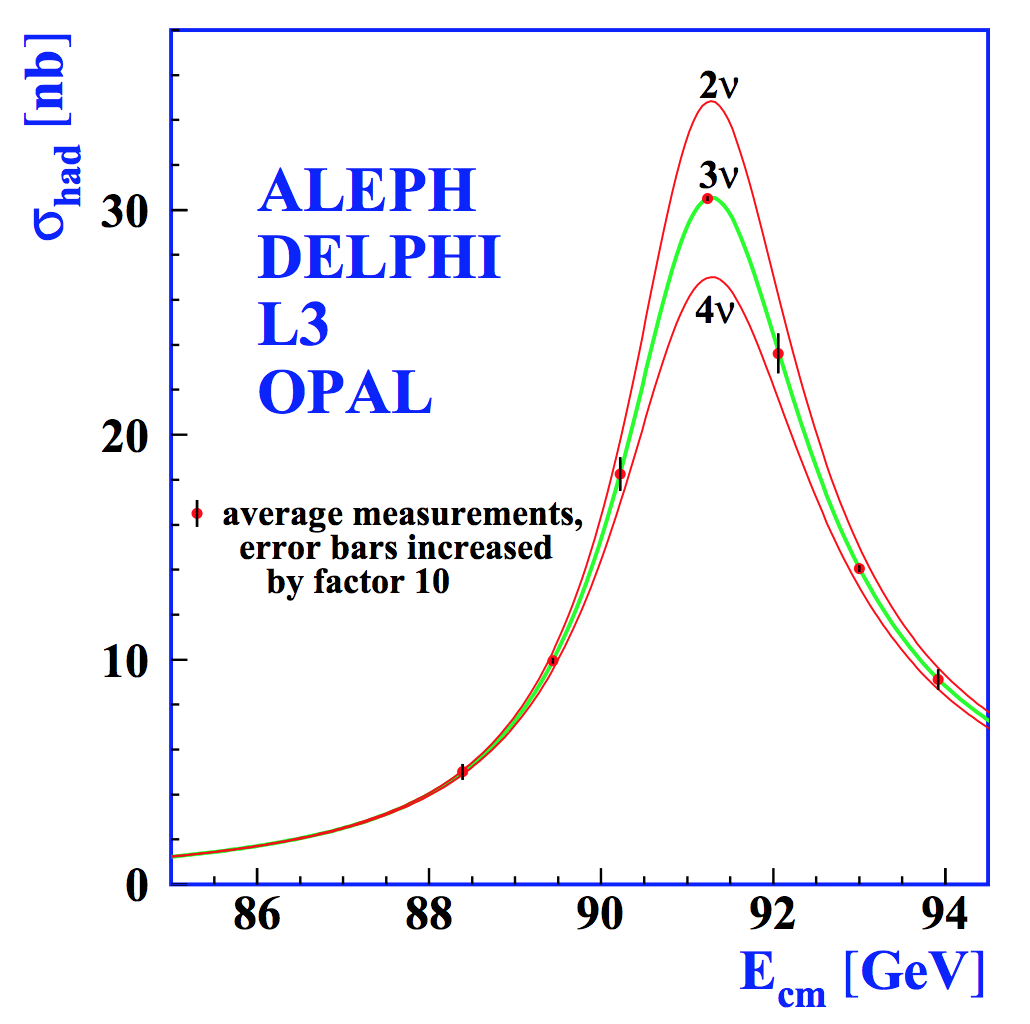
\includegraphics[width=0.5\linewidth]{ALEPH_NumNu.png} 
\caption[The number of neutrinos coupling to the Z from ALEPH]{The number of active neutrinos with a coupling to the Z boson as measured by ALEPH, DELPHI, L3, and OPAL. The data from the four experiments strongly favors only three neutrinos coupling to the Z boson. Image taken from \cite{ALEPH-3Nu}.}
\label{fig:ALEPH}
\end{figure}

\section{History of Cosmic Rays}
\label{sec:cosmic_rays}
In the early years of the 20th century, scientists began investigating previously-unknown ionizing radiation in the atmosphere.
Scientists using electroscopes, early instruments designed to measure electric charge and radiation, discovered low levels of radiation in the air.
This new radiation was observed to be reduced when the electroscope was shielded by metal free of radioactivity, indicating that the signal was not an artifact of the detector itself and was, instead, coming from an external source.

Following just a few decades after the discovery of radioactivity by Becquerel, many scientists believed that the electroscope was detecting radiation from the Earth itself.
The rate would be expected to decrease with increasing altitude above sea level and, to increase with increasing depth in the sea.
Early measurements by Domenico Pacini in 1910 showed that the radiation rate decreased by 20\% at a depth of 3 meters underwater compared to the rate at the surface \cite{Pacini-CRSource}, implying an origin independent of the Earth's crust.
Measurements were performed with electroscopes by Victor Franz Hess in 1912 of the rate of ionizing radiation up to an altitude of 5 km \cite{Hoerandel-CRHistory}.

Hess showed that the observed rate decreased until an altitude of around 1 km, but at a slower rate than expected from theory.
Above 1400 meters, however, the rate of ionizing radiation increased again, rising substantially up to the maximum altitude reached at 5300 meters \cite{Compton-CRAltitude}.
Hess's work, later confirmed by Henri Millikin, showed definitively that there exists a source of radiation of extraterrestrial origin, earning him the Nobel Prize in Physics for 1936 \cite{NobelPrize:1936-Hess}.
This radiation was later dubbed "cosmic rays" by Millikan in reference to their extraterrestrial origin.

\begin{figure}[!h]
\centering
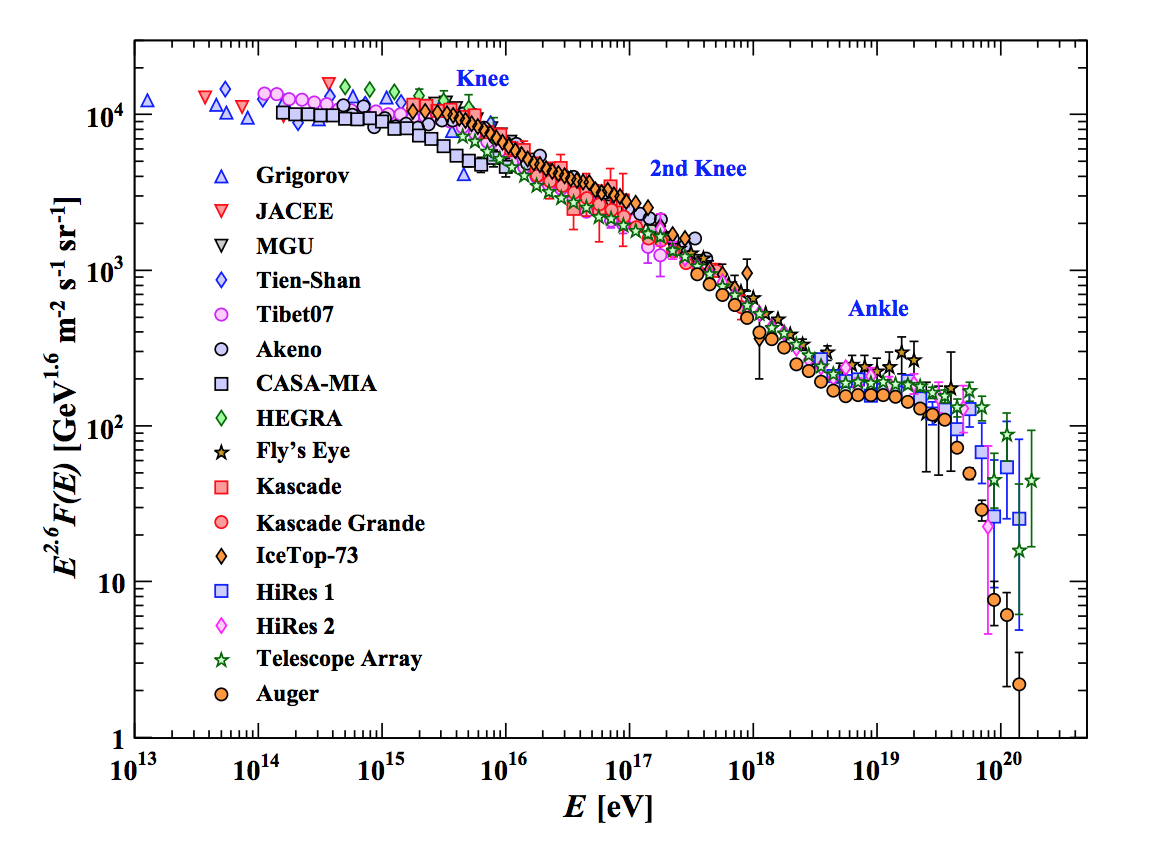
\includegraphics[width=0.9\linewidth]{CR_Spectrum_PDG15.png}
\caption[The cosmic ray spectrum as a function of energy]{The cosmic ray spectrum covers many orders of magnitude in energy and has been verified by many experiments to high precision. The various features are thought to be caused by multiple sources at different scales. Image taken from \cite{PDG-2015}}
\label{fig:CR_spectrum}
\end{figure}

The cosmic rays originally observed by Hess are now known to be primarily composed of protons and helium nuclei reaching the atmosphere from beyond the Earth.
Modern measurements have shown that the cosmic ray spectrum primarily consists of protons with a small contribution from helium and heavier elements \cite{PDG-2015}.
These ions are accelerated in astrophysical sources up to extremely high energies.
The cosmic ray spectrum extends over many orders of magnitude, with the highest energy observations reaching $\mathtt{10^{20}}$ electronvolts - far higher than any Earth-based accelerator.
The spectrum, shown in Figure~\ref{fig:CR_spectrum}, has multiple features that are believed to arise from different accelerator sources at different scales, each of which has been verified by multiple experiments.

Work on cosmic rays has lead to numerous discoveries.
In 1937, the first \emph{hadronic showers} were observed \cite{Blau-HadronicShowers}. 
Hadronic showers of particles created by interactions of cosmic rays were shown to produce large numbers of daughters \cite{Kolhoerster-CoincidenceDetectors, Hoerandel-CRHistory}.
These showers may result in the production of  $5\times10^6$ to over $10^9$ particles each \cite{CosmicRays-Extent}.
These showers begin with a cosmic ray primary particle, often a single proton accelerated to high energies, which interacts with particles of the Earth's atmosphere.
The interaction leads to the creation of various daughters, including muons, pions, kaons, and other hadrons and neutrinos.


\section{Atmospheric Neutrinos}
\label{sec:atmo_nus}
Air showers from cosmic rays provide a useful natural source of neutrinos in the GeV energy range and above that may be used for fundamental physics research.
The hadronic shower produces pions and kaons which decay to produce neutrinos 

\begin{equation}
\pi^+ \rightarrow \mu^+ \nu_\mu \rightarrow e^+ \nu_e \bar{\nu_\mu} \nu_\mu
\end{equation}

from the pions and from the kaons

\begin{equation}
K^+ \rightarrow \pi^+ \nu_\mu \rightarrow  e^+ \nu_e \bar{\nu_\mu} \nu_\mu \nu_\mu
\end{equation}

The resulting neutrino flux depends on a number of parameters, including the Earth's magnetic field and temperature profile, the cosmic ray flux, and the details of hadronic interactions in air showers \cite{Honda-2015}.
The calculation of the neutrino flux predictions requires significant, dedicated simulation work, producing fluxes as both a function of energy (Figure~\ref{fig:honda_en}) and direction (Figure~\ref{fig:honda_coszen}).

\begin{figure}[!h]
\centering
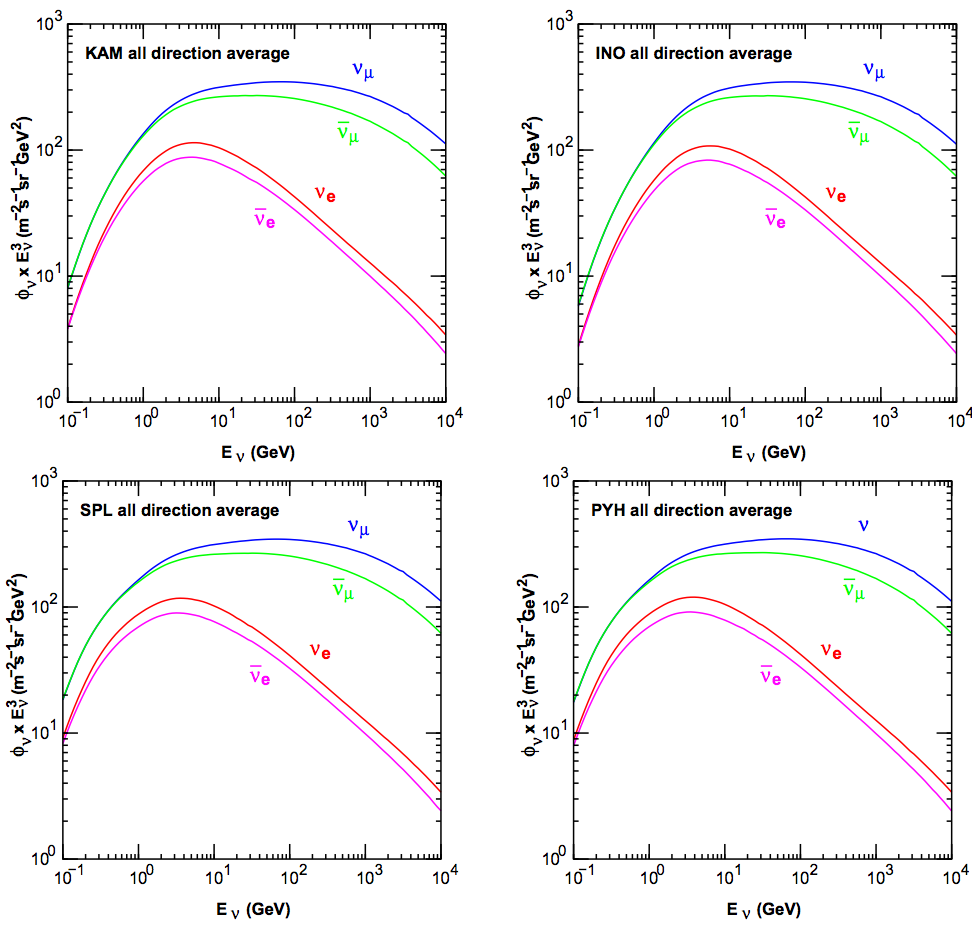
\includegraphics[width=0.6\linewidth]{honda15_en.png}
\caption[Expected neutrino flux as a function of energy]{The expected neutrino flux at Kamioka mine, Japan (Super-Kamiokande, top left), Ino Peak, India (India-based Neutrino Observator, top right), the South Pole (IceCube, bottom left), and Pyhasalmi mine, Finland (EMMA experiment, bottom right) as a function of energy. Note that the neutrino and anti-neutrino fluxes are characterized separately. The differences in the flux at each site is due to differences in the Earth's magnetic field and temperature profile. Figure taken from \cite{Honda-2015}.}
\label{fig:honda_en}
\end{figure}

\begin{figure}[!h]
\centering
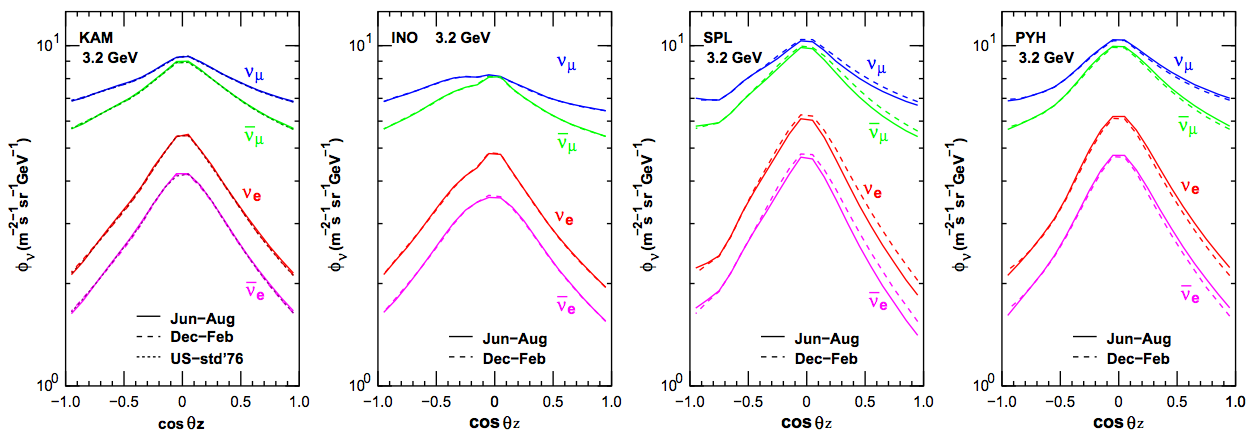
\includegraphics[width=\linewidth]{honda15_coszen.png}
\caption[Expected neutrino flux as a function of direction]{The expected flux of 3.2 GeV neutrinos at Kamioka mine, Japan; Ino Peak, India; the South Pole; and Pyhasalmi mine, Finland as a function of the cosine of the zenith angle. A value of $\cos \theta_Z=-1$ indicates neutrinos passing through the entire Earth and entering the detector from below while a value of $\cos \theta_Z=+1$ indicates neutrinos coming from the atmosphere directly above the detector. The differences in the flux at each site are due to differences in the Earth's magnetic field and temperature profile. Figure taken from \cite{Honda-2015}.}
\label{fig:honda_coszen}
\end{figure}

\section{The Standard Model}
\label{sec:standard_model}

\begin{figure}
\centering
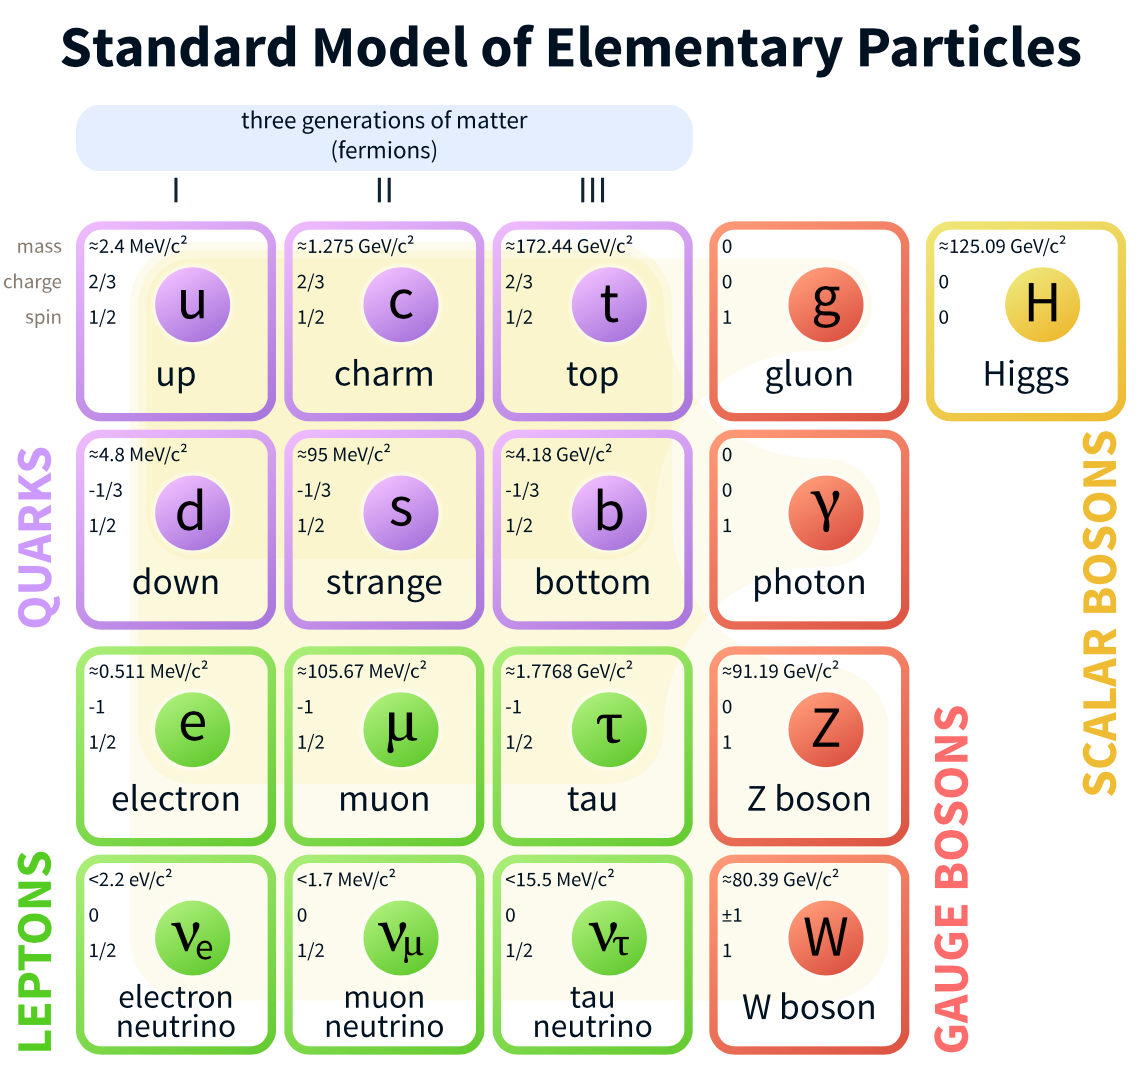
\includegraphics[width=0.7\linewidth]{Standard_Model_of_Elementary_Particles.png}
\caption[The Standard Model]{The Standard Model of particle physics is made up of charged and uncharged leptons, quarks, and the various bosons. Image taken from \cite{StandardModel-Image}.}
\label{fig:standard_model}
\end{figure}

Muons and neutrinos form just a small part of the Standard Model of particle physics.
The Standard Model, with fundamental particle types and properties shown in Figure~\ref{fig:standard_model}, consists of six quarks (up, down, strange, charm bottom, and top), three charged leptons (electron, muon, and tau), three uncharged leptons (electron neutrino, muon neutrino, and tau neutrino), and the five bosons related to interactions (photon, Z, W, gluon, and Higgs).
The Standard Model, developed over the last half century, elegantly encapulates the range of phenomena known to occur in particle physics and has been verified repeatedly over decades by many experiments, yielding precise checks on a wide range of parameters.

The three charged leptons and neutrinos form three "families" or "flavors". 
Each charged lepton is associated with a coupled neutrino which shares a lepton number that is conserved in interactions mediated by the W boson.
The electron, the lightest of the charged leptons at 511 keV \cite{PDG-2015}, is a key ingredient of the atoms that make up the world, is the only stable charged lepton.
The muon, with a mass of 105.7 MeV, is the middle of the three charged leptons, often appearing in particle interactions accompanied by the muon neutrino.
The muon has a relatively long livetime of 2.197 microseconds, far longer than many unstable hadrons.
The tau lepton is the heaviest of the leptons, and with a mass of 1.777 GeV, it is heavier than the proton and appears only in relatively high energy interactions.
The tau has an extremely short lifetime, at 290.6 femtoseconds, and a rich variety of decay products.
This extremely short lifetime and high mass make the tau difficult to produce and study.

For the purposes of this work, the most significant parts of the Standard model are the neutrinos, which will be defined to be signal events; the up and down quarks, which will make up the protons and neutrons upon which the neutrinos will interact; the W and Z bosons, which mediate the weak interactions via which the neutrinos may be observed; and the photon, which gives a method of observation of the interactions.

\subsection{Neutrino Interactions}
\label{subsec:interactions}
In the Standard Model, neutrinos are assumed to be massless, left-handed spin-1/2 leptons which interact solely via the weak force.
The neutrinos may also interact gravitationally, although gravity has no known representation in the Standard Model.
Neutrinos, therefore, are only visible via indirect effects, such as scattering or production of charged particles that may, in turn, give off their own visible signature.
An understanding of the methods by which neutrinos are detected therefore forms an important basis for the study of these elusive particles.
Two basic Feynman diagrams, shown in Figure~\ref{fig:nu_vertex}, represent the two major interaction vertices available for neutrinos.

\begin{figure}
\centering
\begin{tabular}{@{}ll@{}}
\feynmandiagram [vertical=w1 to w2] {
  nue1 -- [fermion, edge label=\(\nu\)] w1 -- [fermion, edge label=\(l\)] e1 ,
  w1 -- [boson, edge label = \(W^{+}\)] w2
}; 
 & \feynmandiagram [vertical=w1 to w2] {
  nue1 -- [fermion, edge label=\(\nu\)] w1 -- [fermion, edge label=\(\nu\)] nu2 ,
  w1 -- [boson, edge label = \(Z\)] w2
}; \\ 
\end{tabular}
\caption[Feynman diagrams for W, Z interactions of neutrinos]{Feynman diagrams showing the interaction vertex of the neutrino with the W and Z boson.}
\label{fig:nu_vertex}
\end{figure}

These two vertices describe the interactions relevent for the work presented in this thesis.
During \emph{charged current} (\emph{CC}) interactions, a $\mathtt{W^{\pm}}$ boson is exchanged between a neutrino and target particle(s), in the process converting the uncharged neutrino to the corresponding charged lepton.
The \emph{neutral current} (\emph{NC}) interactions are those in which the uncharged Z boson is exchanged with the target and the neutrino.
Although the neutrino can change energy and momentum, it does not get converted to a charged lepton.

Detectors used to study particle properties rely on electromagnetic interactions and photons in order to detect particles.
Because the neutrino itself does not interact via the electromagnetic force, charged leptons and hadrons must be used to indirectly study the properties of the incident neutrinos.
Outgoing charged leptons in charged current interactions may be detected, although the direction will not necessarily correspond to that of the incident neutrino. 
The average angle between the incident neutrino and outgoing lepton may be approximated following Equation~\ref{eqn:kinematic_angle},

\begin{equation}
\left<\bar{\theta}_{\nu l}\right> \approx \frac{\mathtt{1.5^o}}{\sqrt{E_\nu \left[TeV\right]}} .
\label{eqn:kinematic_angle}
\end{equation}

There exist three further classifications of neutral current and charged current neutrino interactions in the energy range used in this work: the quasi-elastic, resonant, and deep inelastic interactions \cite{Formaggio-Xsec}.
A fourth type, coherent neutrino scattering, may also occur, although the energies involved are too low to impact this work.
The three types of interactions are contribute to the total cross section with peaks at different energies, as shown in Figure~\ref{fig:xsec}.

\begin{figure}[h]
\centering
\begin{tabular}[b]{c}
  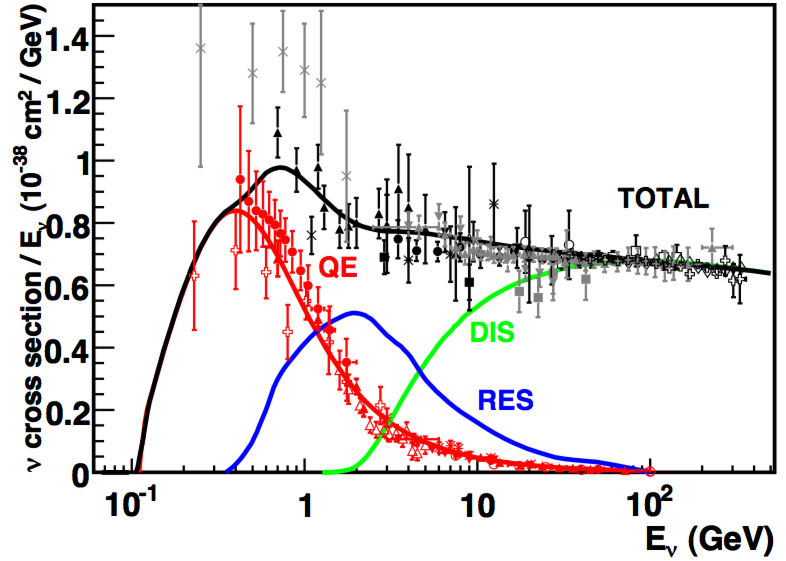
\includegraphics[width=0.45\linewidth]{nu_xsec_formaggio.png} \\
  \small (\textbf{\color{ctcolormain}a}) $\nu$ Interaction cross sections
\end{tabular} \hspace{2pt}
\begin{tabular}[b]{c}
  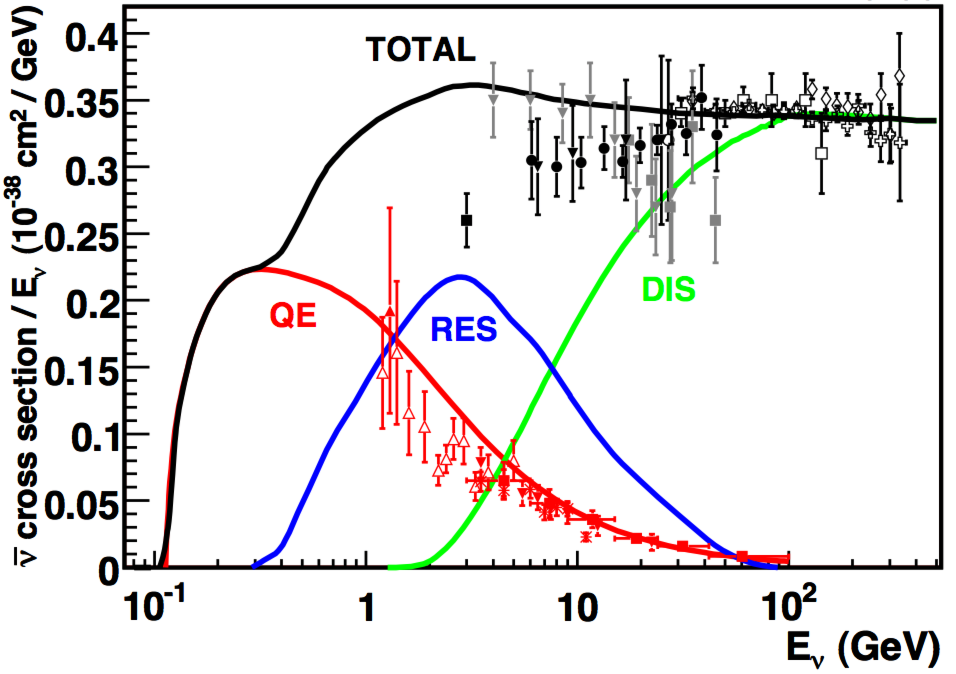
\includegraphics[width=0.45\linewidth]{nubar_xsec_formaggio.png} \\
  \small (\textbf{\color{ctcolormain}b}) $\bar{\nu}$ Interaction cross sections
\end{tabular}
\caption[QE, RES, and DIS cross sections for neutrinos]{The relative contributions to the cross section for $\nu$ (left) and $\bar{\nu}$ (right). The QE events dominate below 1 GeV while the DIS events dominate above 10 GeV. Note the different scales for the neutrino and antineutrinos. Images taken from \cite{Formaggio-Xsec}.}
\label{fig:xsec}
\end{figure}

\subsubsection{Quasi-Elastic and Resonant Interactions}
At low energies of approximately 100 MeV to around 2 GeV, the neutrinos predominantly interact via \emph{quasi-elastic scattering} (\emph{QE}) interactions.
In the QE interaction, the neutrino scatters off an entire nucleon instead of the individual quarks.
In a charged current QE neutrino (anti-neutrino) interaction, the target neutron (proton) is converted to a proton (neutron) while the neutrino is converted to a charged lepton.

The cross section for QE interactions depends on various nuclear form factors that must be fit to experimental data.
Many of these form factors may be fit to electron scattering data, leaving only the axial vector nuclear form factors to be measured in the neutrino sector \cite{Formaggio-Xsec}.
This form factor is normally assumed to have the dipole form 

\begin{equation}
F_A\left(Q^2\right) = \frac{g_A}{\left(1+\frac{Q^2}{M_A^2}\right)^2}
\label{eq:axial_mass_eq}
\end{equation}

where $\mathtt{g_A}$ is a constant fit to experimental data, $\mathtt{Q^2}$ is the 4-momentum transferred in the interaction, and $\mathtt{M_A}$ is the "axial mass".
This last term is fit to experimental data with a value of $\mathtt{M_A = 0.999 \pm 0.011}$ GeV \cite{Formaggio-Xsec}.

\emph{Resonant scattering} interactions (\emph{RES}), which result in the excitation of a nucleon followed by decay via emission of (typically) pions, occur for neutrinos of slightly higher energies of around 500 MeV to 10 GeV.
Resonant interactions are modeled in a similar way as the quasi-elastic interactions, with an associated axial mass term used to describe nuclear uncertainties.

\subsubsection{Deep Inelastic Interactions}
\begin{figure}
\centering
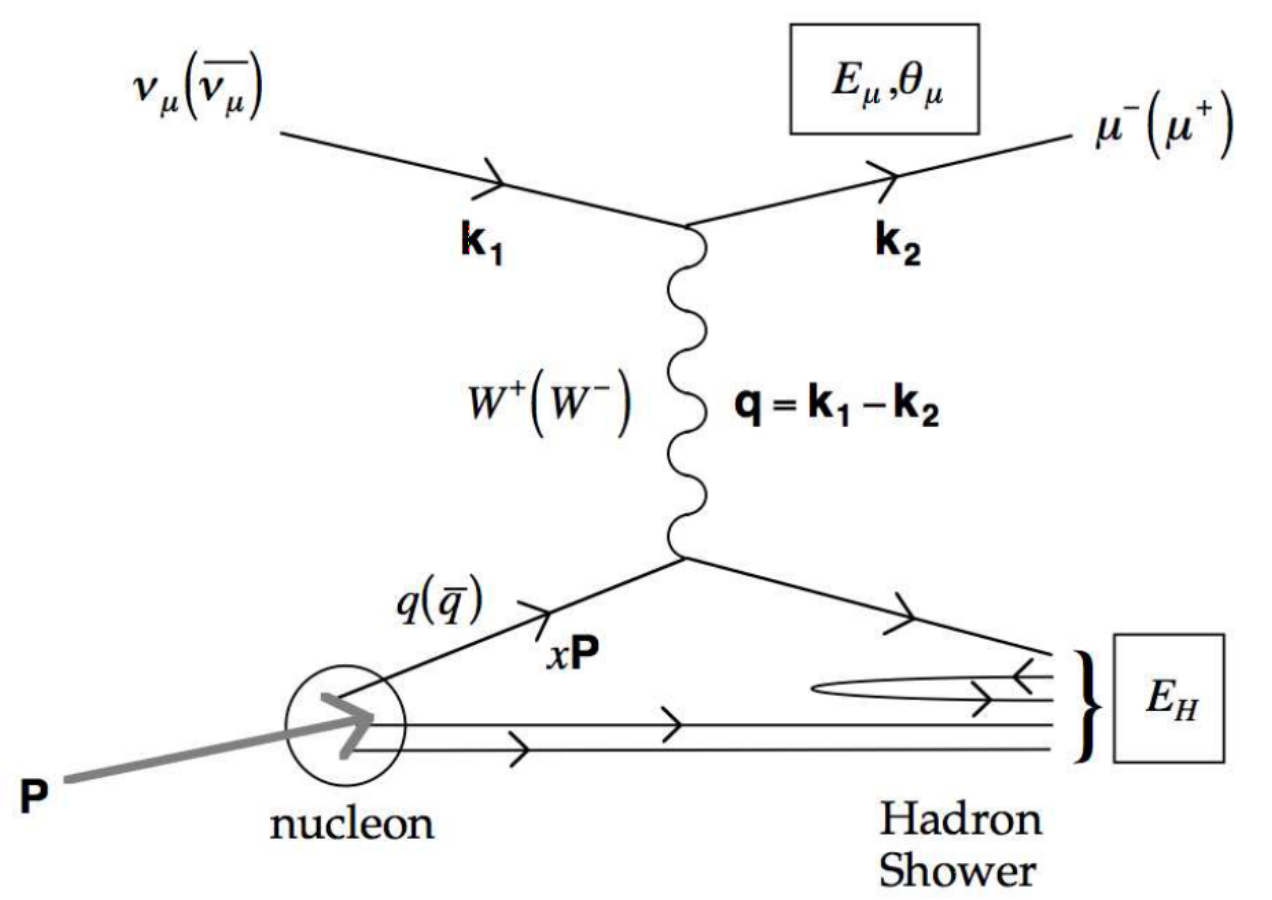
\includegraphics[width=0.5\textwidth]{dis_feynman.png}
\caption[A Feynman diagram of a charged current DIS neutrino interaction]{A Feynman diagram showing an example of a charged current neutrino DIS interaction. An incident muon neutrino interacts with a quark inside of a proton. The result is a hadronic shower as well as a charged muon. Diagram taken from \cite{Formaggio-Xsec}}
\label{fig:dis_feynman}
\end{figure}

Above a few GeV, the neutrino cross section rises approximately linearly with energy and is dominated by \emph{deep inelastic scattering} (\emph{DIS}) interactions.
An example of a DIS interaction is shown in Figure~\ref{fig:dis_feynman}.
In DIS events, the exchange of the Z or W boson probes the internal structure of the nucleons, leading to a scattering off of the individual nucleons.
This results in disruption of the nucleon and the larger nucleus and a collection of daughter particles forming a \emph{hadronic shower}.

As seen in Figure~\ref{fig:xsec}, the DIS process dominates the neutrino cross section above 10 GeV and form the only significant interaction above 100 GeV \cite{Formaggio-Xsec}. 

\section{Methods of Detection}
\label{sec:detection_methods}
Neutrinos may be detected through the QE, RES, and DIS interaction channels.
The interaction of neutrinos at the GeV energy ranges relevent for this thesis lead to the emission of hadrons in a hadronic shower.
The QE interactions at low energies convert neutrons into protons (neutrino) or protons into neutrons (antineutrino) and emitting a charged lepton.
RES interactions excite a nucleon, leading to a deexcitation and emission of particles that can be detected.
DIS interactions produce larger hadronic showers containing many charged particles.

In addition to the hadronic shower, charged current interactions result in an outgoing charged lepton, the result of which depends on the flavor of the incident neutrino.
Outgoing electrons quickly scatter in interactions with the surrounding media, ionizing atoms and producing a secondary \emph{electromagnetic shower} of particles.
Muons, on the other hand, travel longer distances before scattering or decaying in the medium, leading to an extended track.

\begin{table}[]
\centering
\begin{tabular}{@{}lll@{}}
\toprule
Decay                                     & Branching Ratio     & Background   \\ \midrule
$\tau \rightarrow e^- \nu_e \nu_\tau$     & 17.83 $\pm$ 0.04 \% & $\nu_e$ CC   \\
$\tau \rightarrow \mu^- \nu_\mu \nu_\tau$ & 17.41 $\pm$ 0.04 \% & $\nu_\mu$ CC \\
$\tau \rightarrow$ hadrons                & Otherwise           & $\nu$ NC     \\ \bottomrule
\end{tabular}
\caption[Branching ratios for the tau lepton decay]{The branching ratios for the decay of tau leptons. Two-thirds of the time, the tau lepton decays hadronically.}
\label{tab:tau_decays}
\end{table}

The signature of a tau neutrino charged current interaction varies depending on the specific decay channels, shown in Table~\ref{tab:tau_decays}.
Because the tau lepton has a very short lifetime, outgoing taus from charged current tau neutrino interactions tend to decay immediately.

Each of the three decay modes mimic interactions of the electron and muon neutrinos.
The decay to an electron or hadrons produces electromagnetic or hadronic showers respectively.
The secondary electromagnetic or hadronic cascade is theoretically distinguishable from the primary hadronic cascade produced by a tau neutrino charged current interaction, although the distance traveled by the tau lepton at the energies used in atmospheric oscillation measurements, around 10 GeV, is on the order of millimeters.

In each case, the charged particles deposit energy into the interaction medium through a series of stochastic and continuous emissions.
It is through the detection of these stochastic and continuous losses that daughter particles may be identified in the study of neutrinos.

\subsection{Stochastic Emission Mechanisms}
A total of five major stochastic emission mechanisms are important for the energy losses in neutrino experiments \cite{Dima-MMC}:
ionization, bremmstrahlung, pair production, 

The decay of the particle splits the energy of the parent into multiple, lower energy daughters.
Decays of daughter leptons can often by important in the identification of the neutrino flavor, particularly for tau neutrino candidates occuring above 10 TeV when the primary and secondary hadronic interactions become well-separated.

Ionization losses occur when the charged lepton interacts with electrons in the medium, transferring enough energy to librerate the electrons from bound states.
At energies below 1 TeV, these losses are the most significant form of energy loss for charged particles, producing a significant source of additional electrons.
Ionization losses occur roughly independently of the energy of the charged lepton.

Above energies of a few hundred GeV, radiative processes dominate the energy losses for muons in matter \cite{PDG-2015}.
Bremmstrahlung, photon emission from charged particles accelerating in a magnetic field, pair production, in which a particle and antiparticle (typically electron and positron) are created, and hadronic interactions of photons all dominate the energy losses of muons above 1 TeV.

There exists a minimum in the energy loss rates.
Particles emitting near this minimum rate are known as \emph{minimum-ionizing} particles \cite{PDG-2015}.

\begin{figure}
\centering
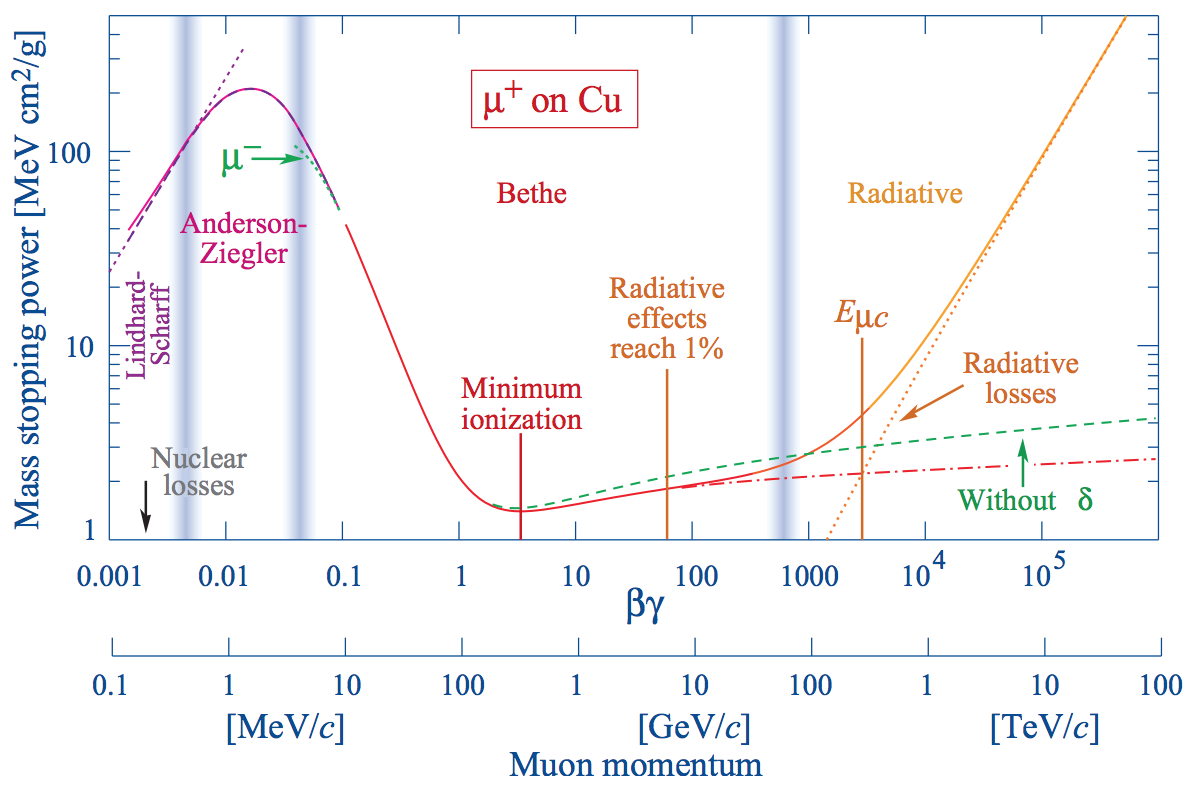
\includegraphics[width=0.8\linewidth]{bethe_bloche-PDG15.png}
\caption[Energy losses of a muon in matter]{An example of the energy loss ($\mathtt{\frac{-dE}{dX}}$) calculated for muons incident on copper. The radiative losses due to bremsstrahlung, pair production, and photonuclear interactions are dominant above 1 TeV. Note the labeled minimum of the curve showing the energy losses of a minimum ionizing particle. Image taken from \cite{PDG-2015}.}
\label{fig:discrete_emissions}
\end{figure}

Stochastic emissions result in additional particles in the detector, leading to improved light yield.
In addition, some detectors use photosensitive emulsions  \cite{Description-OPERA, DONUT-2001}, scintillators \cite{Description-MINOS, Description-NOvA, Description-MINERvA, Description-T2K}, or time projection chambers \cite{Description-ICARUS2} in order to track ionization losses.
These emulsions yield precise characterization of particle decays, allowing experimentalists to uniquely determine the flavor state of the interacting neutrino.

\subsection{Cherenkov Emission}
When a charged particle passes through a dielectric medium with a speed larger than the local phase velocity of light, it will emit \emph{Cherenkov radiation}\cite{Cherenkov-Radiation-Confirmation}.
The effect, first reported by Pavel Cherenkov in 1934 \cite{Cherenkov-Radiation-Observation} remained unexplained theoretically until work done by Ilya Frank and Igor Tamm in 1937 \cite{Frank-Tamm}.

For a dielectric medium, the electric field of charged particle will polarize atoms, inducing a small dipole moment in atoms in the medium \cite{Griffiths-EM}.
The resulting disturbance of the medium propagates with the phase velocity of light, given by the speed of light, \textit{c}, and the index of refraction as a function of the frequency of light, \textit{n(\omega)}.
If the charged particle is traveling faster than the local phase velocity, the electromagnetic disturbance propagates with constructive interference, resulting in a planar wavefront of emission known as \emph{Cherenkov emission}.
The angle of the wavefront relative to the propagation direction is given by the ratio of the distance traveled by the particle and photons in a given time,

\begin{equation}
cos(\theta_C) = \frac{\frac{c}{n(\omega)} t}{v t} = \frac{c}{n(\omega) v} 
\end{equation} 

where $\theta_C$ is the \emph{Cherenkov angle}, $v$ is the speed of the particle.
The energy threshold for Cherenkov emission is set by a combination of the particle mass and the local phase velocity for light, $\frac{c}{n}$.
Using the relativitistic kinetic energy \cite{Tavernier-Particles},

\begin{equation}
\begin{tabular{c}
E_{C} \geq \frac{mc^2}{\sqrt{1-\left(\frac{c/n}{c}\right)^2}} \\ \\

E_{C} \geq mc^2\sqrt{\frac{n^2}{n^2-1}}.
\end{equation}

For ice with a index of fraction of 1.32 at 400 nanometers \cite{ChinesePhysC-2014}, this works out to a minimum energy of 270 keV for electrons and 56.2 MeV for muons.
The number of photons emitted increases with photon energy, with approximately 50\% more photons produced in blue visible light than in red\cite{Tavernier-Particles}
The full emission spectrum, first worked out by Ilya Frank and Igor Tamm in 1937 \cite{Frank-Tamm}, depends on a number of parameters, including the energy and charge of the emitting particle as well as the properties of the medium.
In the case of a particle traveling a distance $L$ much larger than the photon frequency of interest, $\lambda$, the number of emitted photons may be approximated by

\begin{equation}
\frac{dN}{d\lambda}=\frac{2\pi \alpha}{\lambda^2}Lsin^2\theta_C \;\;\; L >> \lambda
\end{equation}

where $\alpha$ is the fine structure constant.

Cherenkov emission is not limited to a single charged lepton. 
All charged particles emit Cherenkov radiation, including any hadrons and charged daughter particles.
While the total amount of energy lost via Cherenkov emission is small relative to losses due to stochastic processes, this emission type is both continous and results directly in photons which may be observed by photodetectors.
This technique is used by multiple experiments, including SNO \cite{Description-SNO}, Super-Kamiokande \cite{Description-SuperK}, ANTARES \cite{Description-ANTARES}, and IceCube \cite{Description-IceCube}.



\label{chapter:oscillations}
\chapter{Neutrino Oscillations}

\label{sec:past_experiments}
\section{Neutrino Experiments: Past and Present}

\label{sec:solar_neutrinos}
\section{Solar Neutrinos: A Hint of Multiple Flavors}

\label{sec:superk_atmo}
\section{Super-Kamiokande and Atmospheric Neutrinos}

\label{sec:oscillation_theory}
\section{Oscillation Theory and the PMNS Matrix}


\label{chapter:detector}
\chapter{The IceCube Detector}
\label{sec:dom}
\section{The DOM: The Basic Unit of IceCube}

\label{subsec:pmt}
\subsection{The Photomultiplier Tube}
\findref{cite https://arxiv.org/abs/1612.05093 over and over and over and over ad infinitum}
The basic unit of the IceCube detector is the \textbf{digital optical module}, often referred to simply as the \textbf{DOM}.
The DOM is designed around a downward-facing 10 inch R7081-02 photomultiplier tube (\textbf{PMT}) from Hammamatsu Photonics. \findref{https://www.sciencedirect.com/science/article/pii/S0168900210006662?via\%3Dihub (remove the backslash in the latex code if pasting the link)}\findref{probably also the hammamatsu documentation http://icecube.wisc.edu/~kitamura/NK/PMT/031112\%20R7081-02\%20data\%20sheet.pdf} and includes onboard electronics for standard operation. 
Circuit boards are included for data acquisition, control, calibration, comminuications and power conversion as well as for high voltage input from the surface.
The electronics of the DOM are encased in a spherical glass housing designed to withstand the high pressures associated with operation in the glacier of Antarctica.
The PMT is optically coupled to the glass housing in order to minimize distortion of incoming light. \findref{something about the gel?}

\needfig{steal figure 3 from the detector paper showing the DOM layout}

\needfig{also grab figure 5 from https://arxiv.org/pdf/1612.05093.pdf for the next section}

A discriminator onboard the DOM is used to identify signals from the PMT with a voltage threshold corresponding to 0.25 photoelectrons.
Each discriminator crossing begins a \textbf{DOM launch}, the lowest level signal available in the IceCube detector containing a digitization of a raw PMT output in the form of a \textbf{waveform}.
Information from the PMT is digitized using the fast analog-to-digital converter (\textbf{fADC}), which provides binned information at 40 megasamples/second for for the 6.4 microseconds following the initial DOM launch.
Simultaneously, the analog signal is recorded by the onboard custom integrated circuits known as \textbf{Analog Transient Waveform Digitizers} (\textbf{ATWDs}) for possible high quality digitization.
Launches are recorded in DOM memory while awaiting a decision from the triggering system.

\label{subsec:LC}
\subsection{Local Coincidence}
If any of the notified DOMs also record a launch within a configurable 1 microsecond window, both launches are said to form a \textbf{hard local coincidence} (\textbf{HLC}) pair.
Nearby DOMs, here defined to be either of the two DOMs above or below the current DOM, are notified of the launch via a signal sent using the \textbf{local coincidence} wiring.
In this situation, all DOMs participating in the HLC begin producing higher quality digitizations from the recorded analog signals using the ATWDs.
Launches which fail to satisfy the local coincidence conditions are referred to as \textbf{soft local coincidence} (\textbf{SLC}) hits.
Launches digitized as part of an HLC pair receive a flag. 
This flag may be used to later identify only those launches which satisfy the local coincident conditions, providing a simple, default method of identifying hits likely to be caused by particle interactions in the detector.

\label{subsec:digitization}
\subsection{Digitization}
Signals from the PMT are digitized using a variety of digitizers.
Each DOM contains two ATWD chips, each of which has access to three amplifier gain levels in order to cover the dynamic range of the PMT.
The highest gain channel is used for most pulses, although lower gains are used in cases of particularly large pulses in order to avoid loss of information due to saturation of the channel.
The ATWD chips sample the waveform at a rate of 300 megasamples/second with 128 samples per launch, recording a total of 427 nanoseconds.
A 10 meter long delay line embedded in the circuitry of the DOM allows the ATWD to record signals from approximately 75 nanoseconds before the discriminator crossing.

When digitizing a signal, the ATWD chip experiences 29 microseconds of deadtime. \findref{https://arxiv.org/abs/0810.4930}
During this time, the secondary ATWD is available to record further pulses, resulting in a total average fractional deadtime per DOM of $\mathtt{2.2 \times 10^{-5}}$ seconds/second.

Examples of digitized waveforms from the ATWD and fADC are shown in \needfig{figure 6 of https://arxiv.org/pdf/1612.05093.pdf}.
Digitized versions of the waveforms are transmitted from the DOM to the IceCube physics data acquisition system (\textbf{pDAQ}) for use in trigger and event building.


\label{subsec:pmt}
\subsection{The Photomultiplier Tube: From Light to Signal}

\label{subsec:digitization}
\subsection{Digitization}

\label{subsec:LC}
\subsection{Local Coincidence}

\label{sec:geometry}
\section{The Geometry of the Detector}

\label{subsec:icecube}
\subsection{IceCube: A Detector for TeV Neutrinos}

\label{subsec:deepcore}
\subsection{DeepCore: Extending the Reach to GeV Scales}


\label{chapter:simulation}
\graphicspath{{chapters/simulation/images/}}
\chapter{Simulation of the IceCube-DeepCore Detector}
\label{chapter:simulation}
In order to model both signal and background, \emph{Monte Carlo simulations} of the detector are necessary. 
In the search for tau neutrinos, this is particularly important due to the low rates and high backgrounds expected, requiring multiple types of simulation for both signal and background.

Simulation in IceCube is broken into three broad stages, each of which will be discussed in turn.
The generators used in the appearance analysis are discussed in Section~\ref{sec:generators}.
The propagation of the charged leptons and photons are then described in Section~\ref{sec:propagation}.
Section~\ref{sec:electronics} describes the simulation of the detector, including the PMT electronics and the detector noise.

\section{Monte Carlo Generators}
\label{sec:generators}

\subsection{Background Generation}
\label{subsec:bg_generation}

\subsubsection{CORSIKA}
\label{subsubsec:corsika}
The primary background for the observation of atmospheric neutrino events is the other particles present in the cosmic ray interactions in the atmosphere.
These interactions produce many particles, most of which are stopped before reaching IceCube by the shielding provided by the Antarctic Glacier.
In order to correctly account for the interactions and decays of these particles, the \emph{CORSIKA} generator from Karlsruhe Institute of Technology is used \cite{CORSIKA}. 

The CORSIKA generator is a collection of code designed to simulate, interact, and propagate a cosmic ray air shower from the interaction point in the upper atmosphere to a user-defined height. 
Originally designed for use with surface detectors such as Auger, HAWC, and IceTop, the code has been adapted for use in the IceCube collaboration by identifying the muon (and, sometimes, neutrino) components of the air shower.

CORSIKA has many modes of operation and options for configuration. 
The standard IceCube simulation of air showers uses the SIBYLL 2.1 hadronization mode \cite{SIBYLL-2.1} to follow the interactions through the shower. 

IceCube simulation of air showers uses two cosmic ray production modes of CORSIKA: the Polygonato and 5-Component modes.

The "Polygonato" mode generates cosmic rays following the model from \cite{Hoerandel-Polygonato}. 
The Polygonato flux parametrized the energy spectra of individual elements of the cosmic ray flux as power laws extrapolated to high energies.
In typical IceCube simulation, CORSIKA simulation produced using the Polygonato mode includes a mixture of muons from all seasons, effectively producing an averaged flux useful under the assumption of equal livetime throughout the year.
The elemental ratios of the generated cosmic ray primaries follow the Polygonato flux directly, producing a "natural" flux of simulated events \cite{CORSIKA}.
The natural spectrum of the Polygonato CORSIKA simulation has the benefit of allowing a direct physical interpretation of the resulting spectrum without the need for reweighting and simplifies the prodution of coincident showers, which require a natural spectrum.

The second model, the five-component mode, reduces the full spectrum of cosmic rays to five effective families: hydrogen, helium, nickel, aluminum, and iron. 
Each of these components is allowed to have a separate normalization and spectral index.
The five-component mode is useful due to the ease with which the user can modify and reweight to different primary spectra, allowing the investigation of different cosmic ray compositions without the production of dedicated simulation.
The simplicity associated with the reweighting of five-component simulation allows IceCube to produce unphysical spectra in order to optimize the production of simulated events necessary for the various analyses.
The five-component simulation may be reweighted to match cosmic ray models, including both the Polygonato model and the newer H3a model, which models the cosmic ray flux using three distinct populations of sources \cite{Gaisser-H4a}.
While this slightly complicates the use of the simulation in analyses, the ability to evaluate the uncertainties in various cosmic ray models has been an invaluable tool for high energy analyses, which can be sensitive to changes in the cosmic ray spectrum above the knee.

About 10\% of the muons from cosmic ray air showers which reach the IceCube detector will arive temporally coincident with muons from other showers.
Five-component CORSIKA simulation, due to the unphysical generation spectrum, cannot easily be used in the production of these \emph{coincident} events and are currently supplemented by the Polygonato CORSIKA for this purpose.

In both cases, the particles from the air shower are only propagated to the surface of the ice. 
For analyses using the in-ice array, we take the muons reaching the surface from a CORSIKA simulation and propagate them through the ice, simulating the continuous and stochastic energy losses along the way. 
The muons are propagated to a surface in the ice consisting of a cylinder with radius 800 meters and length 1600 m centered on the IceCube detector.
In order to reach the detector, a muon must result from a cosmic ray interaction of approximately 600 GeV due to the shielding of the glacier.
Because of this, CORSIKA simulations typically have a lower energy cutoff of about this value to avoid simulating events that will not reach the detector.

In principle, neutrinos may also be produced using the CORSIKA generator. 
In practice, this tends to be extremely inefficient for most searches that are not explicitly looking for muons and neutrinos from the same air showers given the extremely low cross section of the neutrino relative to the muon.
For this reason, the background generation with CORSIKA in IceCube typically refers to muon events only, with no accompanying neutrino.

\subsubsection{MuonGun}
\label{subsubsec:muongun}
CORSIKA simulations are computationally costly and offer few ways to directly control the spectrum of events at the detector.
Targeted simulations in which particular muon samples are required cannot easily be generated with CORSIKA.
In situations where the required muon simulation falls within a relatively narrow phase space, whether that be in energy, angle, or position inside of the detector, it can be beneficial to tailor simulation to the needs of specific analyses.
Alternatively, there are situations in which the details of the cosmic ray interactions are an unnecessary complication to the final level IceCube analyses.
In these situations, IceCube has developed a tool to bypass the full air shower simulation provided by CORSIKA, producing muons directly at a cylindrical surface inside the ice \cite{Thesis-Jakob}.
This tool, known as \emph{MuonGun}, has the benefit of removing the computationally costly simulation of the full air shower, giving the user more control over the resulting simulated events at the cost of information about the initial cosmic ray interactions.
This allows targeted, high statistics background simulation samples to be produced for analyses.

These features of MuonGun give the generator significant flexibility, allowing for a very focused simulation of muons that would not otherwise be possible with the current implimentation of the CORSIKA generator.
As with all targeted generation, there are limitations to the generation scheme.
For example, the settings described above will provide a good description of muons reaching and triggering the DeepCore array, but will not include the correct contributions of muons in the outer IceCube detector.
This can result in disagreement between data and simulation if the limitations are not acknowledged and accounted for.

This abstraction disassociates the muon at the detector from the air shower, and therefore the cosmic ray, that produced it.
In order to properly account for the dependence on the cosmic ray spectrum in the muon weights, dedicated simulations must be produced using the full CORSIKA generator. 
By following the interaction, showering, and propagation to the detector, IceCube is able to produce an effective parametrization of the association between a particular cosmic ray spectrum and the muons reaching the detector.
This must only be done once, but requires a substantial number of simulated events in order to produce a clean parametrization in position, energy, zenith angle, and variables associated with shower multiplicities higher than one.
The version of MuonGun at the time of writing provides the parametrizations for the Polygonato \cite{Hoerandel-Polygonato} and H4a \cite{Gaisser-H4a} cosmic ray spectra. 
At the time of production for the analyses contained hereafter, all MuonGun simulation is produced assuming a multiplicity of 1, meaning that no bundles are yet produced with this generator.
This is a limitation of simulation time: the multiplicity parametrizations vastly extend the parameter space and therefore require significantly more time and effort to handle correctly.

\subsubsection{Accidental Events}
\label{subsubsec:noise_triggers}
While we only observe Cherenkov photons from neutrino and muon interactions in the detector, we also observe a significant component of \emph{accidental triggers} in the DeepCore array.
These events, produced by detector noise in the detector, result in about 40 Hz of triggered events in IceCube, primarily in DeepCore due to the low trigger threshold.
In these events, no actual particle interactions due to muons or neutrinos are observed.
Instead, detector noise alone satisfies the trigger conditions, producing an event.

Production of accidental triggers involves only the noise and electronics simulation.
Because the events occur as a result of random HLC launches in the detector, the simluation requires a special mode, here called \emph{long-frame} simulation, which produces continuous detector readout. 
Breaking the traditional concept of the "simulated event", these simulation sets instead produce a 100 ms long "event" of random detector noise. 
The photoelectrons from the noise simulation are then run through the simulation of PMT and DOM electronics and triggered as a normal simulated event.
After triggering, specialized code is used to divide the long-frame simulation into smaller events similar to standard IceCube experimental readout.

Once the events are generated, weighting the events is relatively straightforward: the weight per event depends on the muon interaction rate and the total simulated time.
The latter is straightforward to calculate, depending only on the number of long frame simulation events produced and the time window for each of these events.
The former is important due to the definition of the accidental triggers. 
These events, by definition, may only occur when no muon or neutrino is interacting within the detector. 
The weight of the accidental triggers must account for this "deadtime" due to particle interactions.
This particle interaction rate in IceCube is dominated by muons with a rate of approximately 2800 Hz, leading to a change in the effective livetime per accidental triggered event of roughly 15\%..

Accidental triggers are computationally expensive to produce, given that they rely on a relatively rare property of random detector noise. 
The production of accidental triggers takes about one hour per minute of simulated livetime, with much of the processing time spent on the simulation of DOMs that do not contribute to final triggered events.
This limits the total effective livetime that can be simulated in realistic timescales.
Current simulations used in this thesis total approximately two months of effective livetime.

\subsection{Signal Generation}
\label{subsec:signal_generation}

\subsubsection{GENIE}
\label{subsubsec:genie}
Background simulation is only part of the Monte Carlo events in IceCube. 
Studies searching for neutrino candidate events require simulated neutrino signal events to infer properties of the original events.

At energies ranging from approximately 1 GeV to 1 TeV, IceCube has adopted the \emph{GENIE} event generator \cite{GENIE}.
This code, used widely throughout the oscillation community, includes information about the various interactions, cross sections, and uncertainties involved in neutrino physics from reactor energies upward.

For IceCube, events in the GENIE generator are produced from a power law energy spectrum with a given spectral index.
These events are then forced to interact with an electron or nucleon within a specified volume with a target density of ice assumed.

The type of interaction is determined using the cross section for the given flavor and energy.
The cross section model, an updated version of GRV98 \cite{GRV98}, includes resonant, elastic, quasielastic, and deep inelastic interactions.
Particles produced in the interaction are propagated out of the nucleus.
GENIE includes final state interactions where hadrons produced in neutrino interaction can reinteract before escaping the nucleus.
Hadrons with energies less than 30 GeV produced in GENIE simulation are propagated individually to obtain the light output using GEANT4 \cite{GEANT4-1,GEANT4-2}.
Above 30 GeV, the lower event-to-event variability permits the use of parametrized light output for hadrons.
GEANT4 is also used to propagate all muons and tau leptons as well as electrons and photons below 100 MeV.

The GENIE code includes tools to reweight events based on uncertainties in eg. the axial masses, cross sections, and various aspects of the interactions themselves \cite{GENIE}. 
These features are used to model uncertainties in the tau neutrino analysis presented in this thesis.

The code is regularly updated, including both new features and retuning of parametrizations to match the latest data.
The events produced in this work use GENIE version 2.8.6.

\subsubsection{Neutrino-Generator}
\label{subsubsec:nugen}
At energies higher than approximately 100 GeV, there are two changes to the simulation code.
At these energies, the contribution to the cross section from deep inelastic interactions becomes dominant while the other interactions become negligible, as expected from Figure~\ref{fig:xsec} \cite{Formaggio-Xsec}. 
This allows the simplication of the cross section calculations with no loss in generality.
In addition, the cross section continues to rise approximately linearly with the energy.
This latter feature requires a detailed simulation of potential interactions far from the detector: namely, high energy neutrinos have a non-negligible chance of interacting while propagating through the Earth.

The \emph{Neutrino-Generator} code (hereafter, \emph{NuGen}) is designed to handle these higher energy interactions \cite{NuGen}.
In this model, neutrinos are no longer produced and forced to interact in the ice directly.
Instead, a neutrino is produced from a power law spectrum in the atmosphere surrounding the Earth.
The event is then propagated through the planet, using the PREM model of the density layers in the Earth \cite{PREM} to simulate potential interactions en route. 
Neutrinos which interact may be lost or may be regenerated following the decay of the daughter particles.
Neutrinos arriving at the detector are then forced to interact in the detector fiducial volume, yielding a simulated event.

NuGen can be configured with various Earth models as well as different generation properties. 
For the studies contained herein, the NuGen files are produced with an $E^{-2}$ spectrum and interact following the CSMS cross section \cite{CSMS}.












\section{Propagation of the Particles and Light}
\label{sec:propagation}
After production of simulated particle interactions, IceCube simulated events require two types of \emph{propagation}.
The first, the propagation of charged leptons and individual hadrons below 30 GeV, produces the energy losses in the detector due to continuous and stochastic emissions.
These energy losses are then used to produce photons that are propagated through the detector using models of the Antarctic glacier.


\subsection{Lepton Propagation with PROPOSAL}
\label{subsec:proposal}

\begin{figure}
\centering
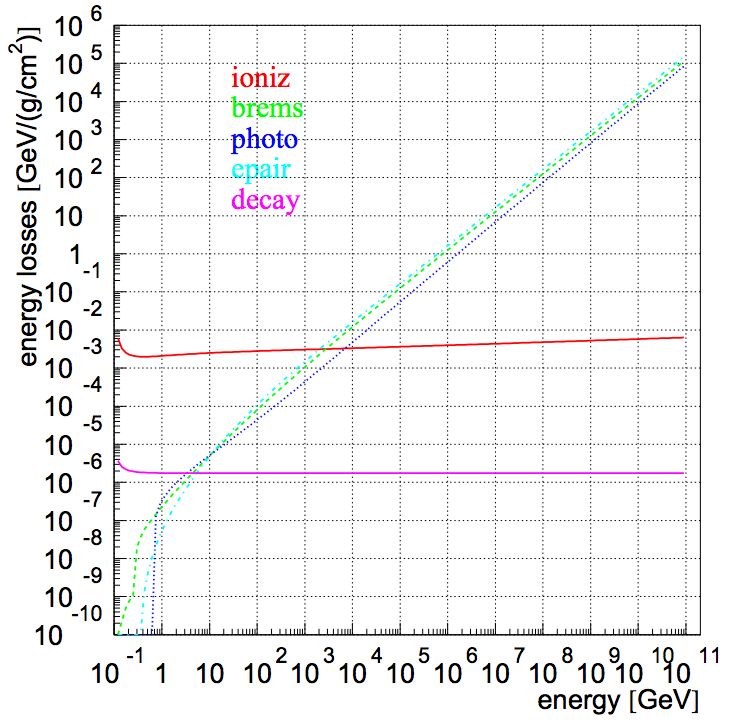
\includegraphics[width=0.6\linewidth]{discrete_emissions_MMC.png}
\caption[Energy losses for a muon in ice]{Average energy losses ($\mathtt{\frac{-dE}{dX}}$) for a muon in ice. At very low energies, ionization losses dominate. Above approximately 1 TeV, pair production and photonuclear effects become more important. Image taken from \cite{Dima-MMC}}
\label{fig:discrete_emissions}
\end{figure}

In IceCube, leptons and hadrons not propagated using GEANT4 are propagated by \emph{PROPOSAL}, a software package containing parametrizations of the ionization, electron pair-production, bremsstrahlung, photonuclear interactions, and decay processes of particles in ice \cite{PROPOSAL}.

PROPOSAL propagates the charged particles through the detector, simulating these processes to give energy emissions along the path of each particle.
The eenergy losses of particles  in the ice is handled by parametrizations as a function of particle energy as shown in Figure~\ref{fig:discrete_emissions}.


\subsection{CLSim for Photon Propagation}
\label{subsec:clsim}
Once the energy deposition for each particle simulated with GEANT4 and PROPOSAL, the resulting photons must be produced and propagated. 
There exist two modules which can handle this: Photon Propagation Code \emph{PPC} and OpenCL Simulation Code \emph{CLSim}. 
The differences are largely of implementation details and both have been verified to give identical results.
Only the latter, CLSim, will be discussed here.

CLSim is a code designed to propagate emitted photons using ray tracing algorithms \cite{PPC}.
The independence of the individual photons is leveraged to perform the propagation of all photons in parallelized calculations using the OpenCL programming language \cite{OpenCL}.
Photons are then propagated through the ice with the model of the scattering and absorption properties, continuing until they are either absorbed or until they reach a DOM.
Photons which reach DOMs are stored to be used in the simulation of the IceCube PMTs.

The propagation of individual photons is efficient at low energies, where the scattering of individual photons is important.
At energies above a few hundred GeV, the light yield is large enough that the propagation of individual photons is both excessively costly as well as unnecessary.
In those cases, a feature known as \emph{oversizing} is used by setting a \emph{oversize factor}, $N_{OS}$.
The oversize factor, often set to 5 for IceCube simulations above 1 TeV, allows for the production of \emph{weighted photons}.
These weighted photons each represent $N^2_{OS}$ individual photons, reducing the number of particles to propagate by $1/N^2_{OS}$.
In order to compensate for the bundling of photons, the effective radius of the DOM is also increased by $N_{OS}$.

Oversizing is efficient for the simulation of high energy events with large numbers of photon.
This breaks down at GeV energies, where the photon flux from an event is low and scattering or absorption of individual photons matters.
Because of the complications associated with oversizing at low energies, most simulations of DeepCore events are done with the oversizing features disabled.

\subsection{Angular Acceptance and Hole Ice}
\label{subsec:holeice_sim}

\begin{figure}
\centering
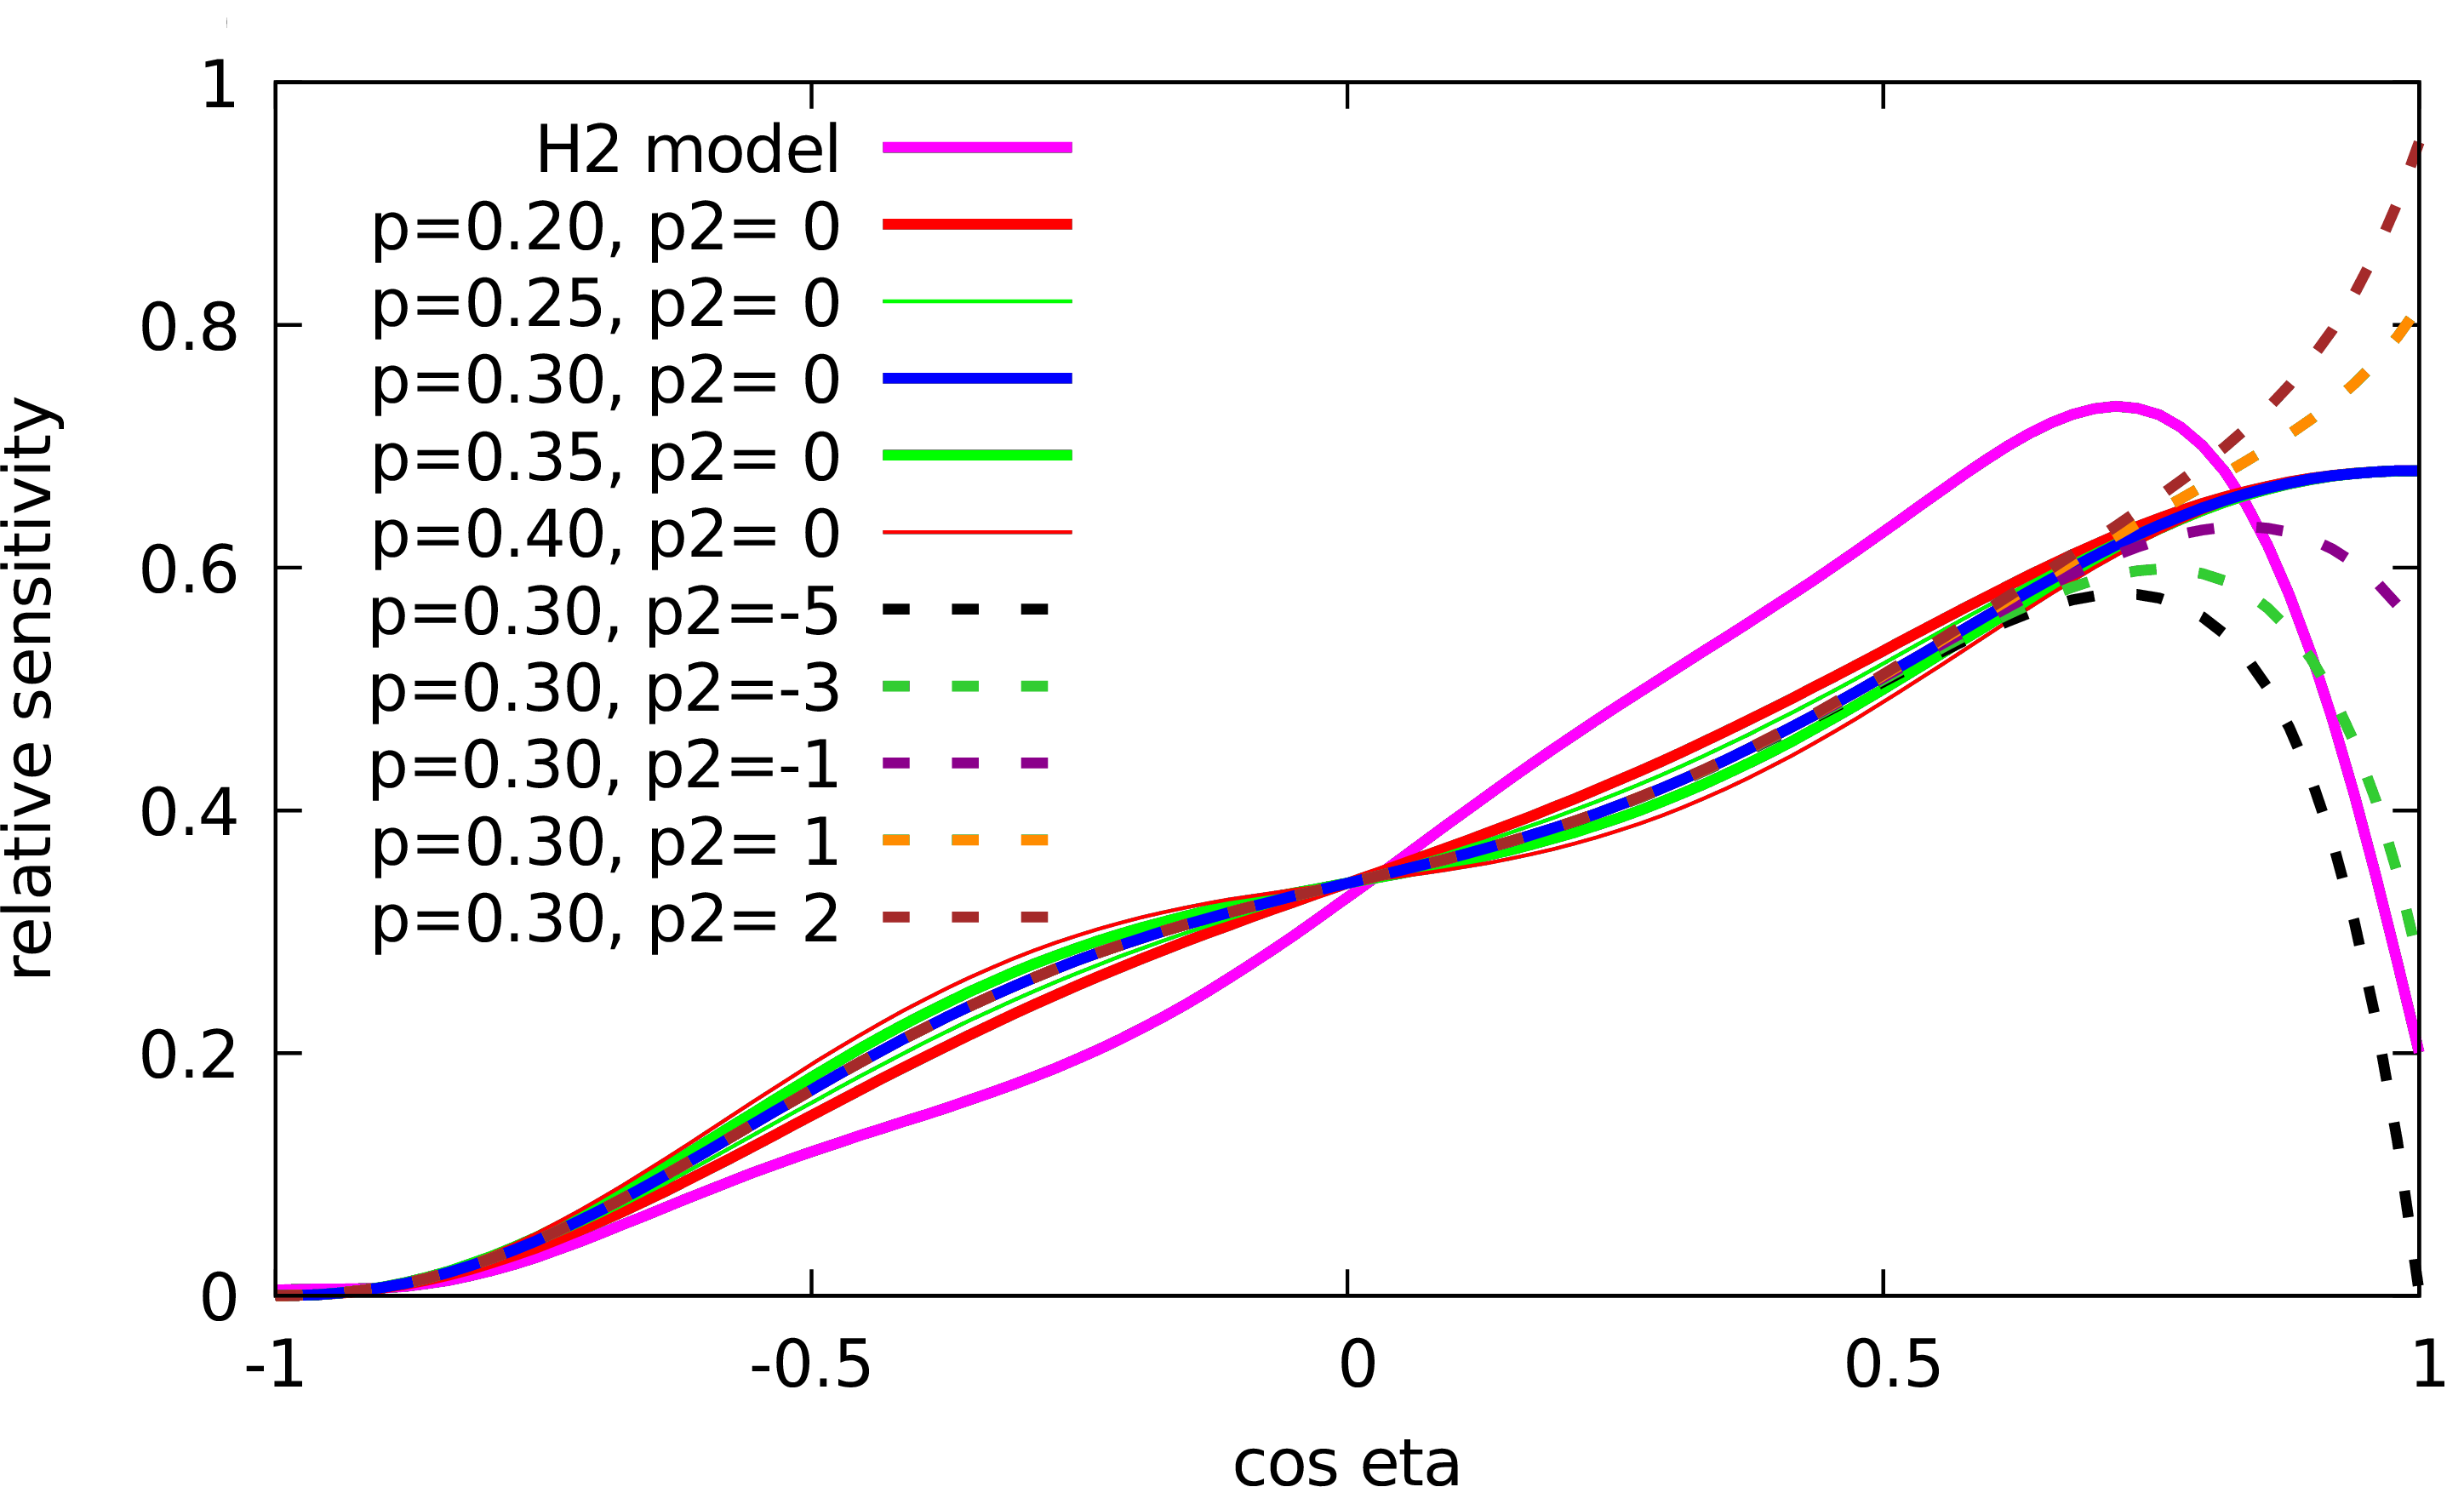
\includegraphics[width=0.7\textwidth]{angular_acceptance.png} 
\caption[Angular acceptance models for IceCube hole ice]{Examples of the angular acceptance models used by IceCube. The relative sensitivity as a function of arrival direction is shown with cos(eta)=-1 indicating the back of the PMT and cos(eta)=1 the face. The variation of the acceptance model used for this search is shown by varying two parameters in the model. The 'p' parameter primarily controls the acceptance at the side of the DOM while the 'p2' parameter controls the acceptance from the forward region. A second model, H2, is also shown.}
\label{fig:angular_acceptance}
\end{figure}

When photons reach the surface of a DOM, the \emph{angular acceptance} is applied in order to model the impact of the hole ice.
This acceptance, calculated from a combination of lab and in-situ measurements, represents the PMT efficiency as a function of the photon arrival direction.
The acceptance has a negligible efficiency for photons arriving from the back of the PMT and higher efficiency for photons reaching the face of the PMT as shown in Figure~\ref{fig:angular_acceptance}.
All other directions follow a curve between these two points.
The angular acceptance model used in this thesis uses an empirical form fit to flasher data with two free parameters, as shown in Figure~\ref{fig:angular_acceptance}.
The most forward (downward-facing) direction in the PMT, shown with $cos(\eta)$~=~-1, is most affected by the bubble column (see Section~\ref{sec:hole_ice}). 














\section{Simulating the Detector Electronics}
\label{sec:electronics}

\subsection{Noise within IceCube-DeepCore}
\label{subsec:noise_sim}
The noise simulation module used in IceCube, known as \emph{Vuvuzela}, models the Poissonian and non-Poissonian detector noise using a set of five  parameters, each representing distinct processes \cite{Thesis-Vuvuzela, Description-IceCube}. 

The \emph{thermal noise} and \emph{radioactive decays} are Poisson processes simulated using rates fit to each DOM.
The thermal rate is correlated with the temperature and forms a large component of the noise in IceCube DOMs, with a typical rate of 200 Hz while the decay rate has a typical value of 50-100 Hz due to radioactive activity in the DOM glass.
The noise model produces photoelectrons at the photocathode of the PMT simulation.

In order to model this bursting behavior described in Section~\ref{subsec:noise}, an effective mode is used which represents the timing of consecutive noise  using a log-normal distribution. 
This introduces three additional parameters to the noise model: the average number of photoelectrons emitted during a "burst", giving the normalization; the mean time between photoelectrons within a burst; and the standard deviation of the timing within a burst. 
The non-Poissonian component to the noise model produces an additional 400 Hz of noise \cite{Thesis-Vuvuzela}.
Noise photoelectrons in simulation are added as additional charge on each DOM at the face of the PMT.

The Vuvuzela model has previously been fit to each DOM in the detector, although with some limitations. 
Work completed during this thesis, discussed in Chapter~\ref{chapter:vuvuzela}, improved the calibration of the noise model.

\subsection{PMTResponseSimulator and DOMLauncher}
\label{subsec:pmtsim}
The IceCube detector does not directly measure photoelectrons emitted from the photocathode. 
Instead, IceCube events record the voltage response from the PMT via the output waveform.
The production of simulated waveforms from incident photons is produced by a pair of software modules.

\begin{figure}
\centering
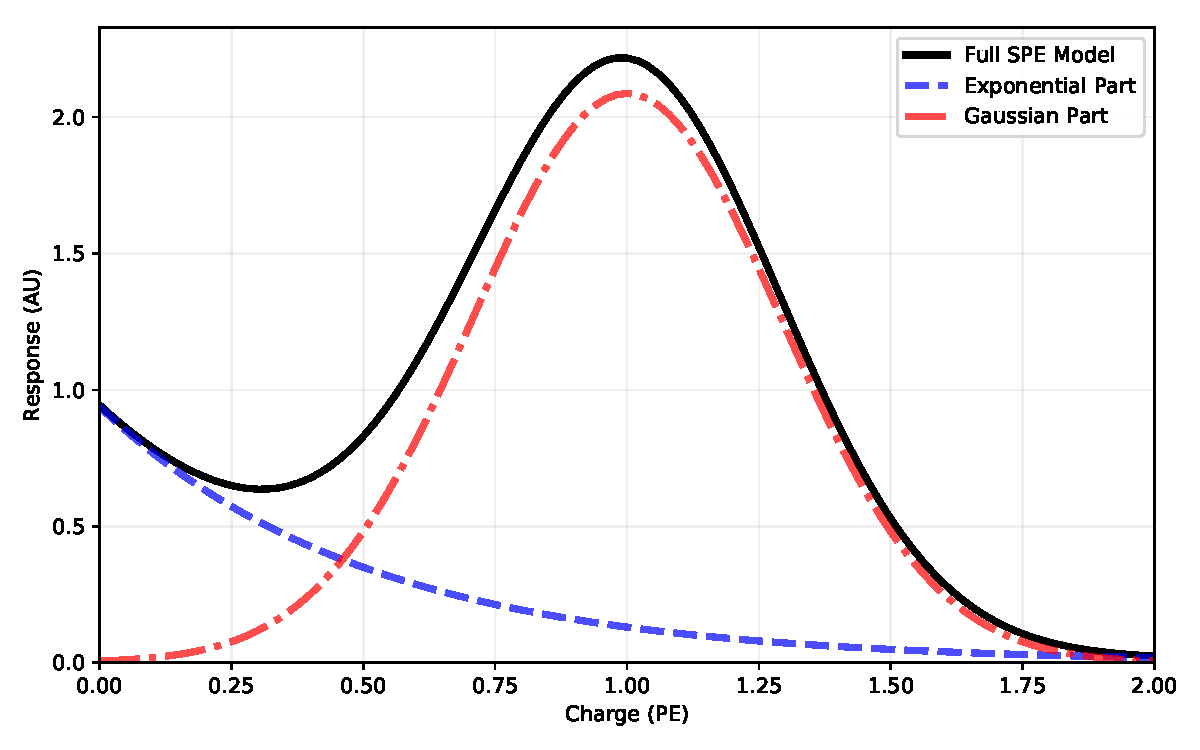
\includegraphics[width=0.7\textwidth]{ta0003.pdf} 
\caption[The SPE template used in IceCube simulation]{The SPE template used in Monte Carlo simulation. The gaussian (red, dash-dot) and exponential (blue, dashed) parts of the full model (black) are shown. The SPE template is used as a sampling distribution for each incident photon in order to determine the observed charge. The SPE template is used for all DOMs.}
\label{fig:ta0003}
\end{figure}

The first module, \emph{PMTResponseSimulator}, simulates the amplification process of the PMT, including the effects of pre-, late-, and afterpulsing.
Each of these three effects is modeled using calibration measurements performed in the lab \cite{IceCube-PMT}.
PMTResponseSimulator also calculates the amount of charge recorded by the DOM from each incident photon reaching the photocathode by sampling from the \emph{single photoelectron} template (\emph{SPE} template).
The SPE template used in simulation generation is calculated from lab measurements of 118 DOMs prior to deployment \cite{TA0003}.
The template, shown in Figure~\ref{fig:ta0003}, is represented by the sum of an exponential and gaussian term and is applied identically to all DOMs.

Prepulses, late pulses, and afterpulses are applied in a recursive process, which every incident hit having a probability of 0.3\%, 3.5\%, and 5.93\% to produce each respectively.
These probabilities were measured in the lab and are used for all DOMs. 

The second module, \emph{DOMLauncher}, handles the local coincidence circuits, simulation of the DOM clock, the discriminator, and digitization.
The triggering system is then applied following the description of Section~\ref{subsec:triggers}.






\label{chapter:vuvuzela}
\chapter{Updates to the Noise Simulation}
The search for tau neutrinos is a search for rare particles near the detector threshold.
Under these conditions, the search requires excellent understanding of threshold effects and detector behavior.
In order to better model the detector, the noise simulation used in IceCube was updated with improved measurements after the discovery of disagreements in charge variables.
This process is described in this chapter.

The chapter begins by describing the process used in previously to fit the Vuvuzela noise model for each DOM in Section~\ref{sec:old_vuvuzela}.
The limitations of the previous fitting process and the discovery of new disagreements is discussed in Sections~\ref{sec:vuvuzela_limitations} and \ref{sec:lowdt_vuvuzela} respectively.
The new fitting procedure is then described in Section~\ref{sec:vuvuzela_fitting}.
New results of the fitting procedure are then discussed in Section~\ref{sec:vuvuzela_newfits}.

\label{sec:old_vuvuzela}
\section{A Summary of Previous Fits}
Detector noise is a nuisance in most physics and astronomy experiments.
PMT noise is assumed to be due to random emission from the photocathode and is affected by the gain of the PMT.
Noise pulses from PMTs appear uniformly in time as a Poisson process.

The Poissonian noise model was used in the past in IceCube. 
With the introduction of the lower trigger threshold in DeepCore in 2010, however, it became clear that additional unsimulated sources of noise exist \cite{Thesis-Vuvuzela}.
These additional hits appeared to occur in 'bursts' on a single PMT extending for up to a millisecond.
Due to the time-correlations of these hits, the phenomenon was labeled \emph{correlated noise}.

The Vuvuzela model, described briefly in Section~\ref{subsec:noise}, is now used to model both the Poissonian and non-Poissonian noise in IceCube.
The empirical model consists of a Poisson process for electronic noise and radioactive decays and a correlated component modeled with a log-normal distribution.
The model contains five free parameters per DOM.
Ten minutes of untriggered data from the detector, dominated by noise hits, was used for calibration of the Vuvuzela parameters.

The Vuvuzela noise model is fit using the distributions of the time between subsequent hits, shown previously in Figure~\ref{fig:noise_model}.
Fits for each DOM were performed using the Pearson chi-squared test statistic between the data histogram, $d$, and the simulated histogram, $m$.

\begin{equation}
\chi^2 = \sum_i^{bins} \frac{\left(d_i-m_i\right)^2}{m_i}
\end{equation}

\begin{figure}[h]
\centering
\begin{tabular}[b]{c}
  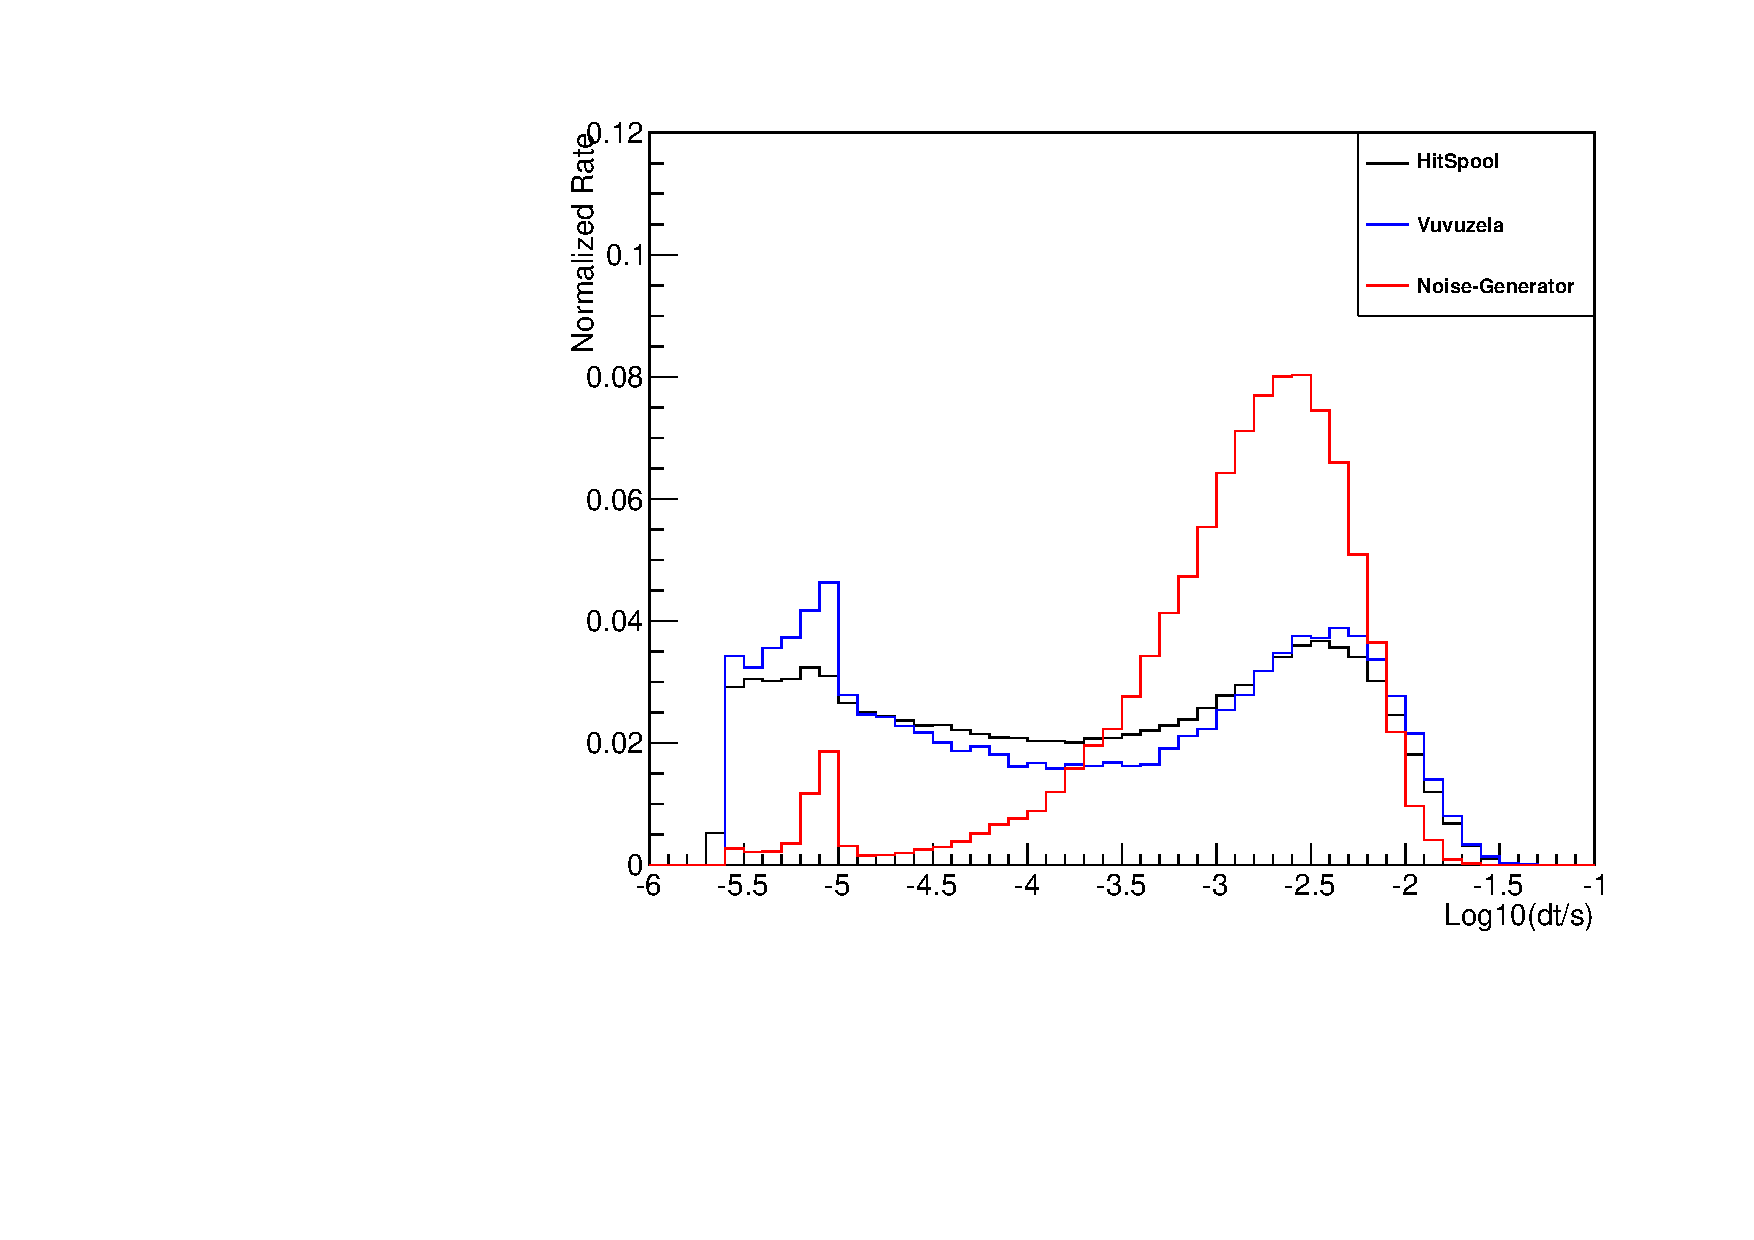
\includegraphics[width=0.45\linewidth]{old_dom_11-19.pdf} \\
  \small (\textbf{\color{ctcolormain}a}) DOM 11-19
\end{tabular} \hspace{2pt}
\begin{tabular}[b]{c}
  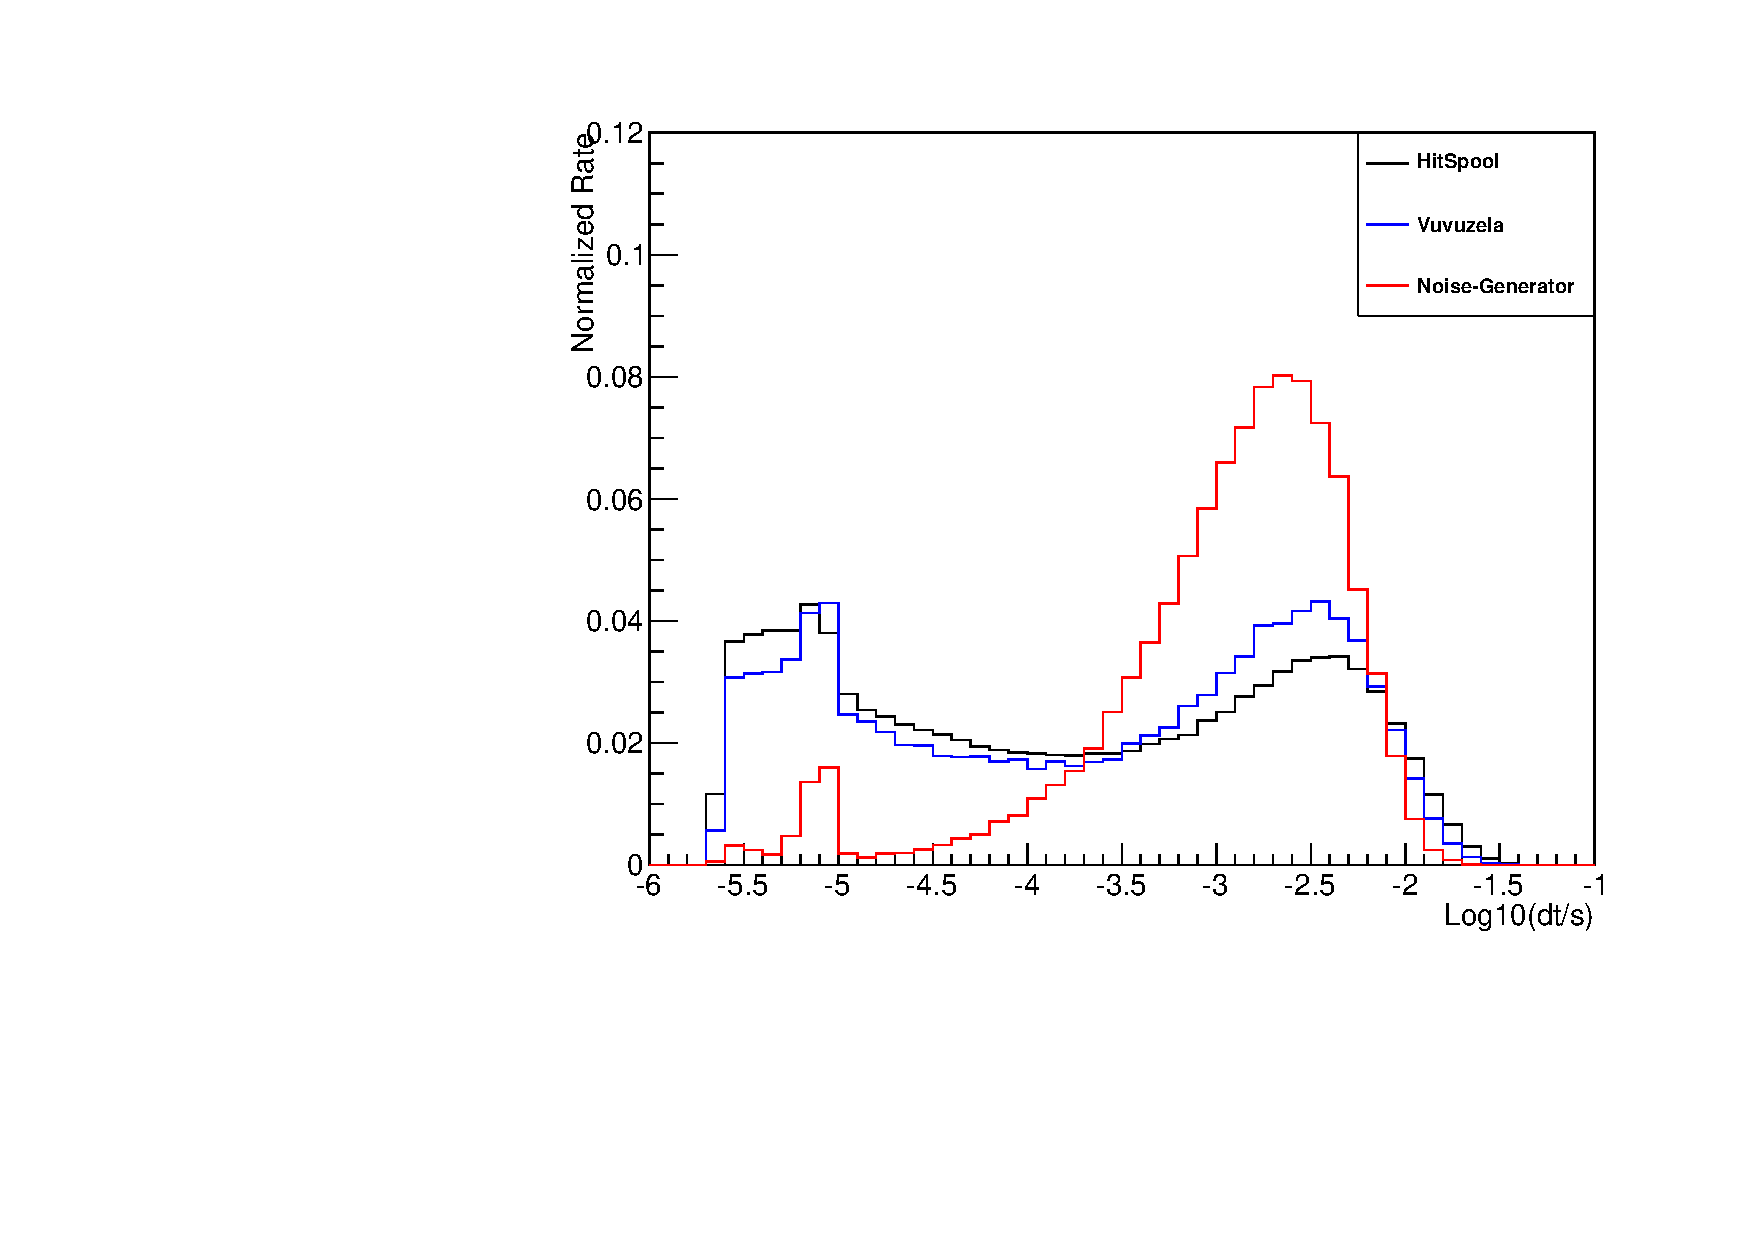
\includegraphics[width=0.45\linewidth]{old_dom_83-42.pdf} \\
  \small (\textbf{\color{ctcolormain}b}) DOM 83-42
\end{tabular}
\caption{Two examples of the original calibration work for the Vuvuzela model. The distribution of the time ("dt") between hits is shown. In black, untriggered detector data is shown. In red, a purely Poissonian noise model is shown. An afterpulsing peak is visible at $10^{-5}$ s. The Vuvuzela model is shown in blue. The Vuvuzela model shows improved agreement with data at all timescales.}
\label{fig:old_vuvuzela_fits}
\end{figure}


The value of the $\chi^2$ was minimized using a Metropolis-Hastings algorithm \cite{PDG-2015}.
For each iteration of the algorithm, new parameters were selected and the response of the DOM was resimulated using PMTResponseSimulator and DOMLauncher.
Each fit was computationally intensive, requiring between two and four CPU-weeks for each DOM.
Due to the computationally requirements of the fits, the stopping condition was intentionally loosely defined, with a goodness-of-fit of 10\% used.

\begin{figure}
\centering
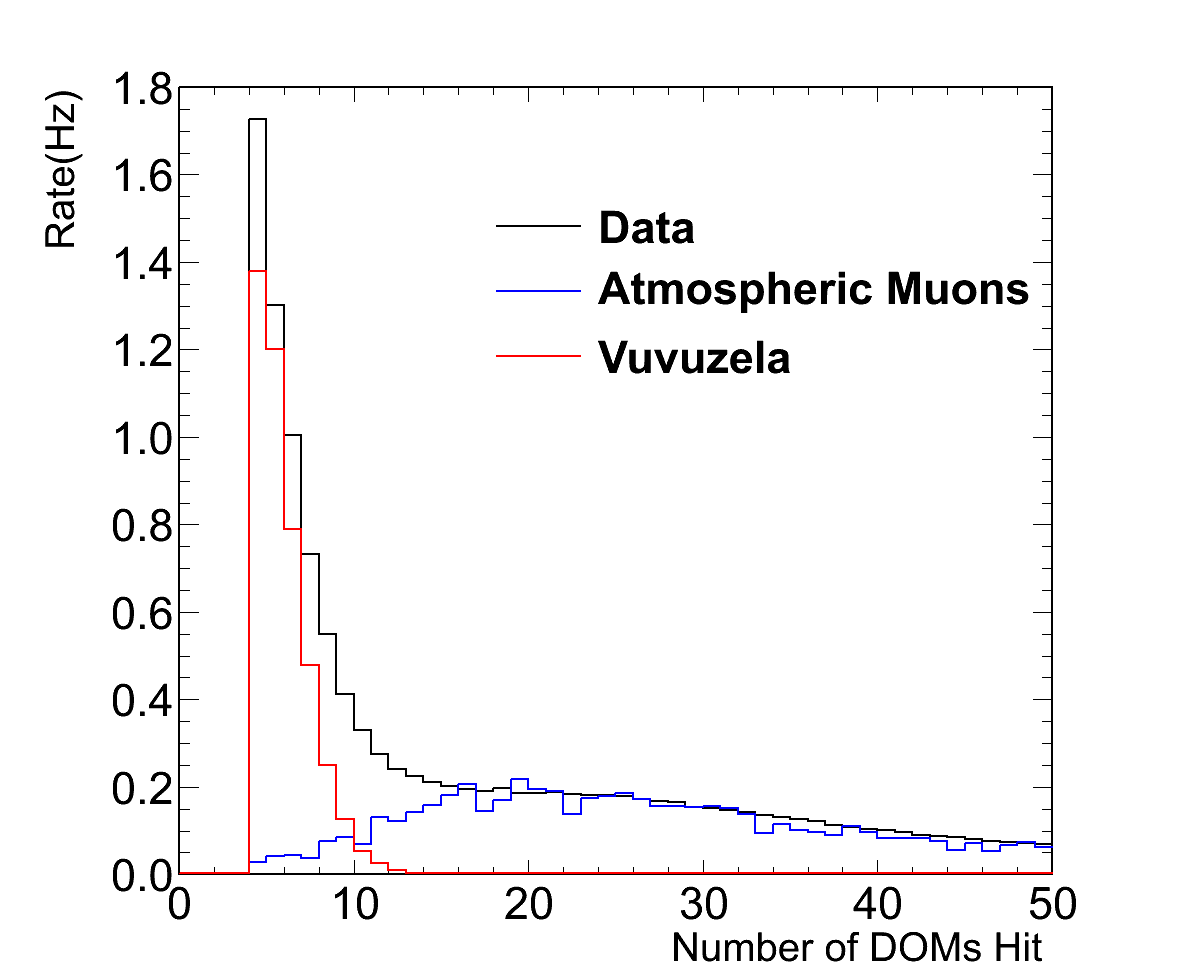
\includegraphics[width=0.6\textwidth]{srtwofflinepulsesdc_withnoise_vuvuzela.png} 
\caption{The rates of events in DeepCore as a function of the number of hit DOMs in a cleaned hit series. The data, shown in black, consists of two components: the accidental triggers (red) and the atmospheric muons (blue). Accidental triggers produced using the Vuvuzela noise model reproduce most of the rate of events below 10 hit DOMs, although a rate disagreement remains. Image from \cite{Thesis-Vuvuzela}.}
\label{fig:old_nch}
\end{figure}

Two examples from the original calibration work are shown in Figure~\ref{fig:old_vuvuzela_fits}.
The Poissonian noise model used previously is shown for comparison.
The Vuvuzela model more accurately reproduces the observed data across all timescales.
Distributions of the number of hit DOMs and the number of accidental triggers due to detector noise, shown in Figure~\ref{fig:old_nch}, improve significantly after inclusion of the updated noise model \cite{Thesis-Vuvuzela}.

\label{sec:vuvuzela_limitations}
\section{Limitations and Disagreement with Previous Fits}
While accidental triggers with the Vuvuzela model better reproduced the rates observed in data, Figure~\ref{fig:old_nch} showed disagreement between data and simulation at very low numbers of hits.
This region of the parameter space is dominated by accidental noise triggers in simulation.

An evaluation of the limitations of the previous calibration was performed in 2014, uncovering a number of possible improvements.
The original fits were limited due to a number of factors. 
For example, the fits excluded the effect of atmospheric muons in the detector under the assumption that the hit rate per DOM due to atmospheric muons (approximately 5 Hz) is significantly smaller than the noise hit rate observed in previous calibration (about 600 Hz).
Potential issues may arise from this assumption, which was not tested during original calibrations, including any potential time-correlated hits associated with muons.

Furthermore, some fits resulted in potentially-incomplete minimization.
Due to the nature of the fit distributions, there existed significant degeneracy in the parameter space, leading to further difficulties.

During the fitting process, the strength of the afterpulsing peak at 9 microseconds was discovered to differ between DOMs.
This effect was unsimulated, leading to convergence problems when fitting this region.
In response, fits were artificially limited to timescales longer than 10 microseconds, allowing the minimizer to only observe part of the correlated noise distribution.

Because the noise hits are unlikely to satisfy the HLC conditions, timescales smaller than 6.4 microseconds were unavailable for investigation.
No checks were performed for the Vuvuzela model below this limit..
The noise model itself was used down to 2 microseconds, however, resulting in uncertainty due to the extrapolation of the noise model to shorter times.
The limit of 2 microseconds was implemented due to the inherent difficulty in characterizing effects at these timescales due to artificial deadtime related to the HLC launch readout. 

\label{sec:lowdt_vuvuzela}
\section{Low-dt Noise from Vuvuzela}
In an attempt to address the imposed simulation limit at 2 microseconds, a new version of the Vuvuzela code, was created with this cutoff removed.
The resulting noise, labeled \emph{low-dt} noise for the short timescales ($\Delta$t), was used to produce a simulation of accidental noise triggers and CORSIKA muons for testing without further calibration.

\begin{figure}[h]
\centering
\begin{tabular}[b]{c}
  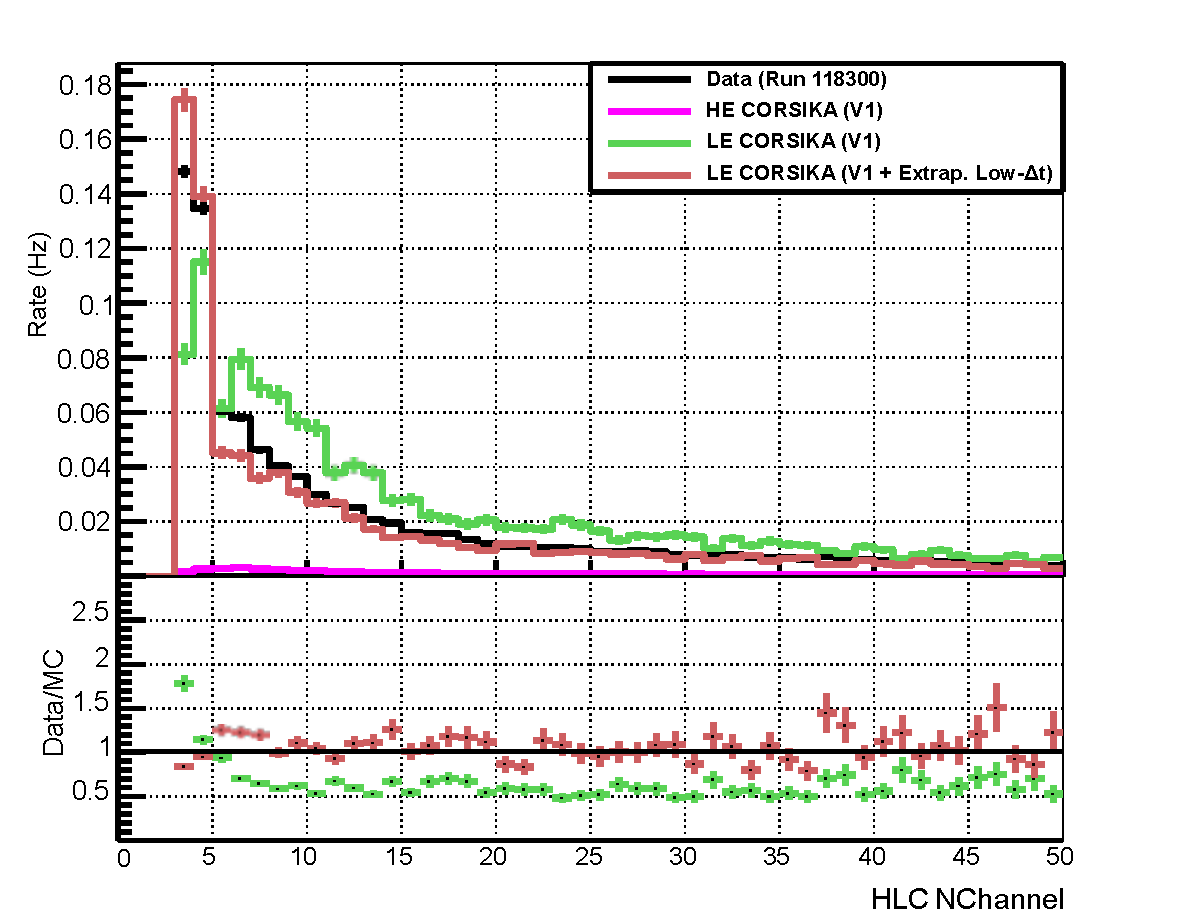
\includegraphics[width=0.45\linewidth]{old_HLC_NChannel.pdf} \\
  \small (\textbf{\color{ctcolormain}a}) HLC hits in DeepCore Events
\end{tabular} \hspace{2pt}
\begin{tabular}[b]{c}
  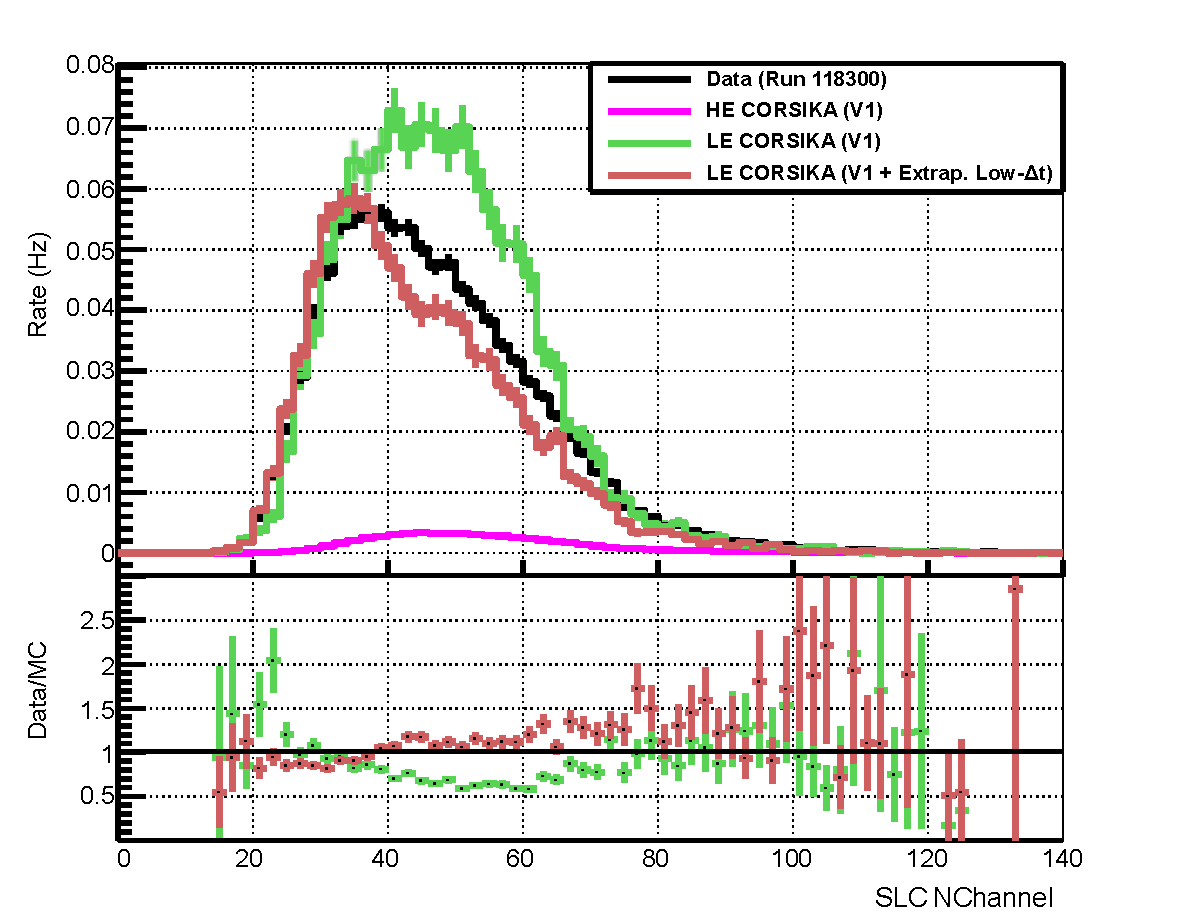
\includegraphics[width=0.45\linewidth]{old_SLC_NChannel.pdf} \\
  \small (\textbf{\color{ctcolormain}b}) SLC hits in DeepCore Events
\end{tabular}
\caption{The number of hit DOMs satisfying the (a) HLC and (b) SLC criteria described in Section~\ref{subsec:LC}. The distribution from 8 hours of data (black) is shown compared to a sample of CORSIKA muons at low-energy (600 GeV $\leq E_{primary} \leq$ 100 TeV) and high energy (100 TeV $\leq E_{primary} \leq$ 100 EeV). The addition of the low-dt extension to Vuvuzela improves the agreement between data and simulation in both HLC and SLC distributions.}
\label{fig:uncalibrated_nchannel}
\end{figure}

The first tests, shown in Figure~\ref{fig:uncalibrated_nchannel}, used the number of hit DOMs in DeepCore events to evaluate the effect of the low-dt noise extension.
The number of accidental triggers, dominant for events with fewer than 5 HLC hits, increased with the additional noise hits.
The number of muons, which make up the majority of events with more than 10 HLC hits, decreased due to the use of the DeepCoreFilter, a veto described in further detail in Section~\ref{subsec:DeepCoreFilter}.
Both effects led to improved agreement between data and simulation.

\begin{figure}[h]
\centering
\begin{tabular}[b]{c}
  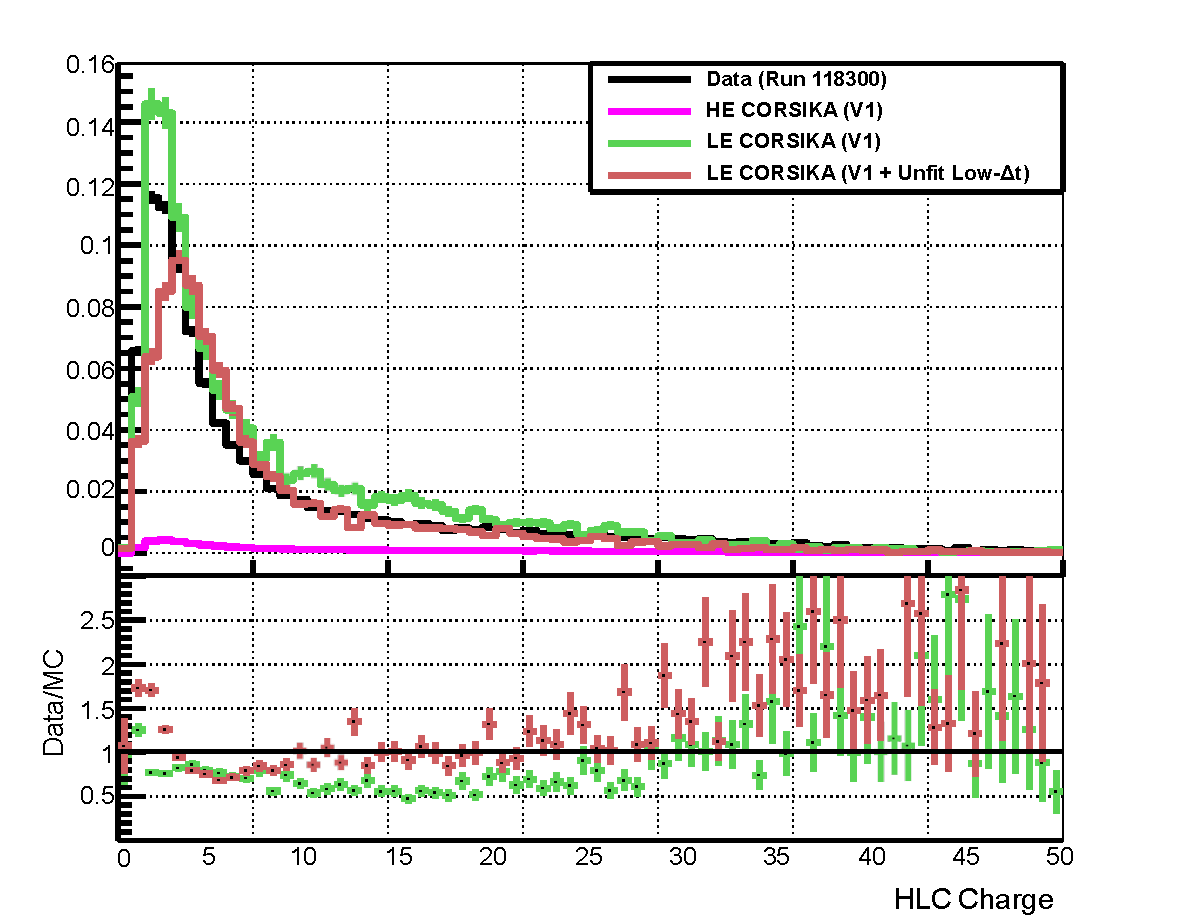
\includegraphics[width=0.45\linewidth]{old_HLC_Charge.pdf} \\
  \small (\textbf{\color{ctcolormain}a}) HLC Charge in DeepCore Events
\end{tabular} \hspace{2pt}
\begin{tabular}[b]{c}
  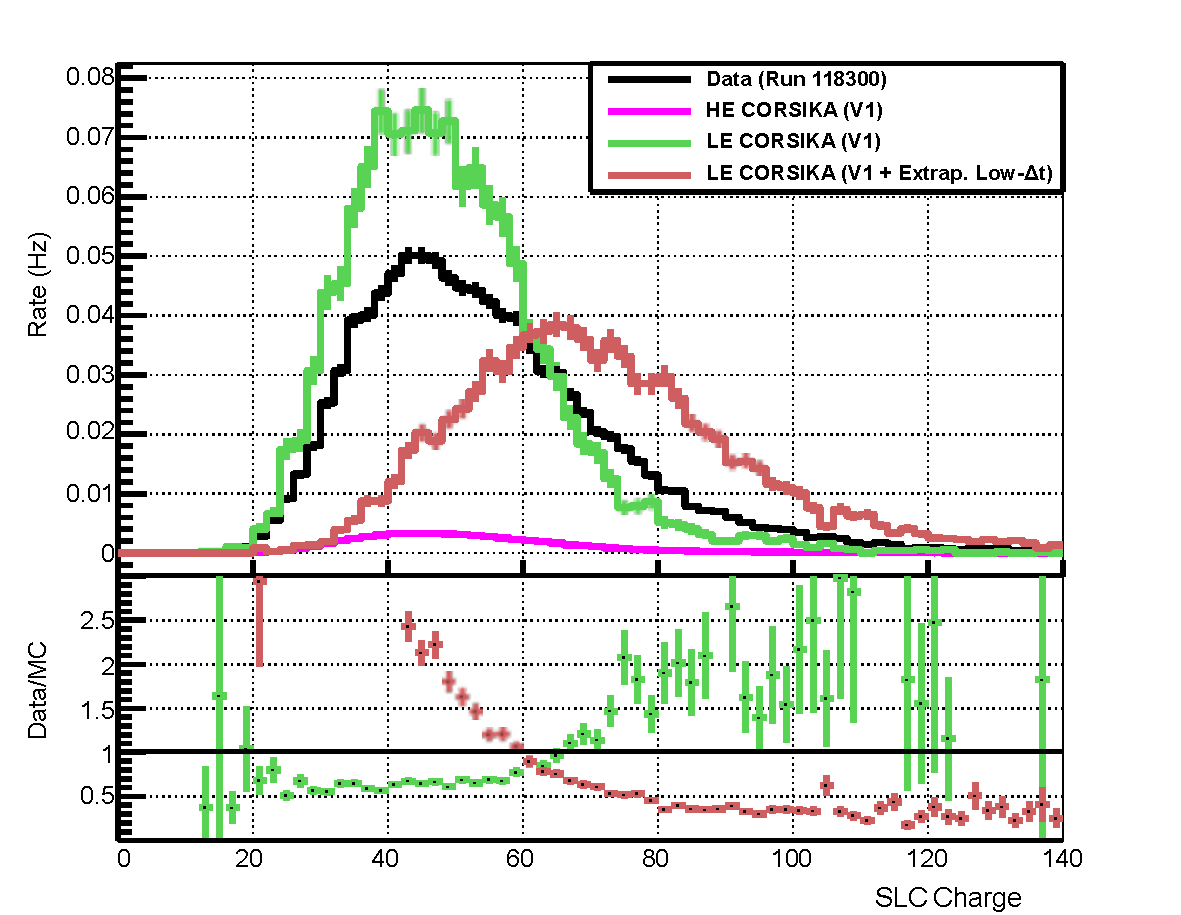
\includegraphics[width=0.45\linewidth]{old_SLC_Charge.pdf} \\
  \small (\textbf{\color{ctcolormain}b}) SLC Charge in DeepCore Events
\end{tabular}
\caption{The total amount of charge on DOMs satisfying the (a) HLC and (b) SLC criteria described in Section~\ref{subsec:LC}. The distribution from 8 hours of data (black) is shown compared to a sample of CORSIKA muons at low-energy (600 GeV $\leq E_{primary} \leq$ 100 TeV) and high energy (100 TeV $\leq E_{primary} \leq$ 100 EeV). Unlike in Figure~\ref{fig:uncalibrated_nchannel}, the charge distributions using the low-dt extension to Vuvuzela shows large disagreements with data. This is most visible in the SLC charge distribution.}
\label{fig:uncalibrated_charge}
\end{figure}

Because the extended noise model adds hits occuring at timescales down to nanoseconds, multiple hits can occur within one waveform, leading to increased observed charge.
When the noise distribution is extended below 2 microseconds, the tail of the distribution falls into the ATWD window of 322 nanoseconds, increasing the charge of noise hits in HLC DOMs.
Furthermore, some fraction of the hits in a burst of correlated noise occur within the three bins recorded from the FADC for SLC hits.
The result is that SLC hits due to noise no longer occur as single-photoelectron pulses, as is the case when noise hits are rare at the 10 nanosecond timescales, but as an integration of multiple single pulses.
Such an effect would be most visible in the charge distribution of SLC DOMs, which are more likely to be due to noise hits than HLC DOMs.

The total charge of DOMs associated with HLC and SLC hits was evaluated to look for this effect due to the extended noise model.
The result is shown in Figure~\ref{fig:uncalibrated_charge}.
The change in the charge is observed clearly in the SLC charge distribution, where a systematic shift is visible due to the low-dt extension.
Both the original Vuvuzela model and the extended Vuvuzela model show significant disagreement with data in the SLC charge distribution.
This demonstrated that the noise distribution at very short timescales was an important effect that deserved further attention.

\begin{figure}[h]
\centering
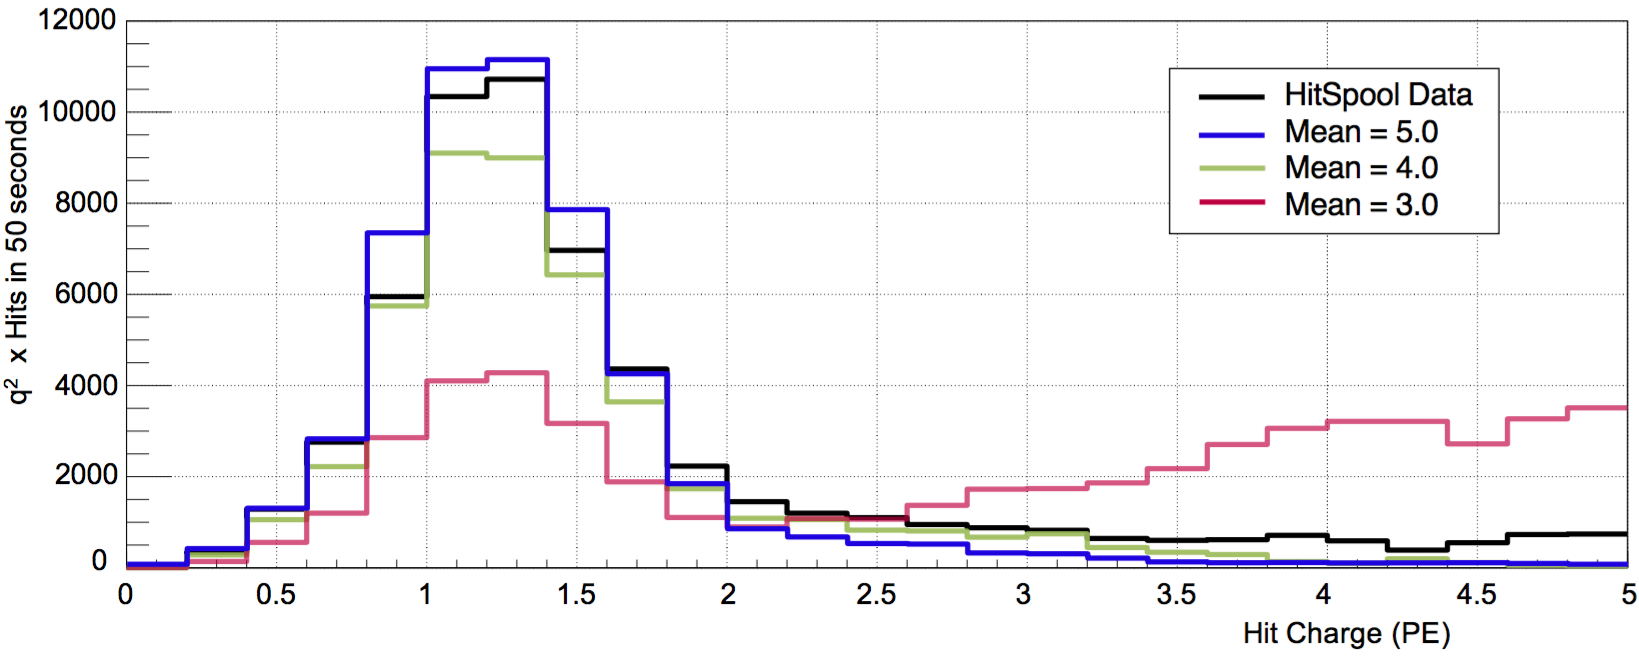
\includegraphics[width=0.5\pagewidth]{lowdt_charge_effects.png} 
\caption{The effect of changing the noise distribution parameters on the charge. Note the scale of the y-axis, which is scaled in order to emphasize the effect. Here, the gaussian mean is shifted from "5" (100 microseconds) to "3" (1 microsecond). All other parameters are held constant. By moving the correlated noise distribution to shorter timescales, more of distribution falls into one FADC bin, increasing the charge output for each launch. }
\label{fig:lowdt_effect_charge}
\end{figure}

The observed effect of the low-dt extension on the SLC charge distribution indicates that the distribution is sensitive to the region below 2 microseconds.
The charge distribution of each DOM may therefore be used in the fitting procedure in order to characterize the low-dt end of the noise timing distribution.
The effect, demonstrated in Figure~\ref{fig:lowdt_effect_charge}, allows the investigation of a part of the distribution unavailable in previous fits.

\label{sec:vuvuzela_fitting}
\section{Updating the Fitting Code}
The effect of the low-dt extension on the charge distributions indicated the potential for improvement in the noise model distribution.
New calibration fits for the updated the noise model, referred to as \emph{Vuvuzela V2} fits, were planned to include this extension for all DOMs.

With the opportunity to refit, a number of additional improvements were implemented.
The afterpulsing peak at 9 microseconds was explicitly included in the fitting code.
To account for the variability in the strength of the peak, a scale factor for the afterpulsing was included in the Vuvuzela V2 fits.

In order to include the effect of atmospheric muons, a set of Polygonato CORSIKA.
The Polygonato model was selected due to the natural weighting scheme of the output files, allowing continuous simulation of the detector.
Simulated files were divided into 10 microsecond long events (\emph{long-frame} events), each containing multiple muons.
The simulation was halted after photon propagation, giving a collection of muons without detector noise and effects applied.

\begin{landscape}
\centering
\begin{figure}
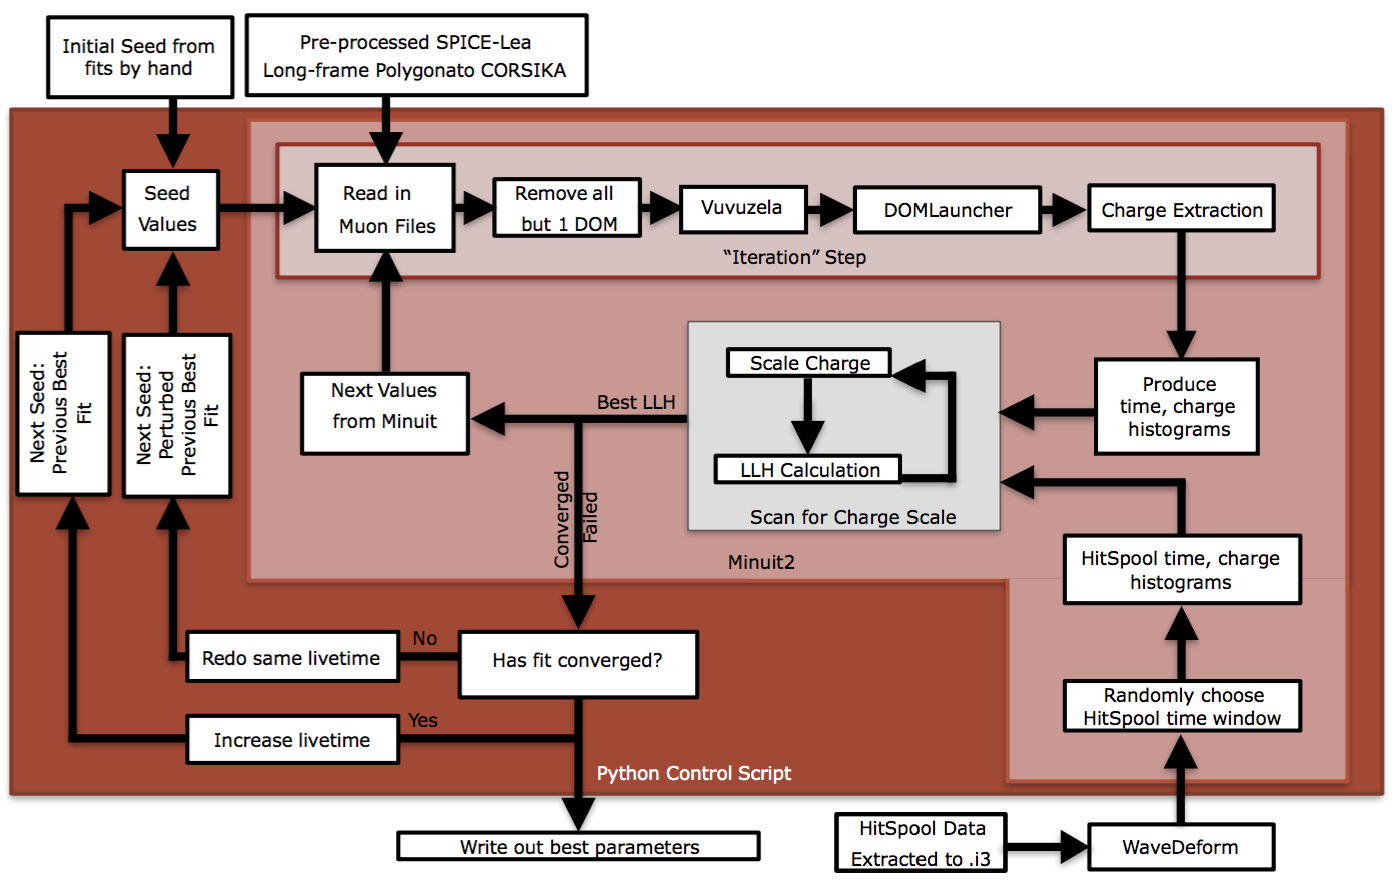
\includegraphics[height=0.8\textwidth]{fit_flowchart.png} 
\caption{A schematic diagram of the process used in the Vuvuzela V2 calibration fit.}
\label{fig:fit_flowchart}
\end{figure}
\end{landscape}

The fitting process, described schematically in Figure~\ref{fig:fit_flowchart}, is divided into several parts. 
The code started with untriggered detector data as well as the produced long-frame CORSIKA events. 
The fit included a total of six explicit parameters: the five parameters from the original Vuvuzela model as well as a scale factor for the afterpulsing.
Later investigations led to the introduction of a charge scale parameter to account for systematic differences between the data and simulated charge.
Seeds for each parameter were taken from the Vuvuzela V1 calibration fits from 2012.
Fits were performed for each DOM in parallel.

For each iteration, the long-frame CORSIKA files were filtered to remove information on all DOMs not currently being fit.
The noise and detector simulation were applied using the current parameter set for the iteration.
Charge extraction from the waveforms was performed using standard IceCube tools.
After the simulation for a given set of parameters, histograms were produced for untriggered data and simulated hits.
As in the previous fits, the time between subsequent hits is used as the primary observable of the noise behavior.
In addition, the observed charge on the DOM is used as a second observable.

\begin{figure}[h]
\centering
\begin{tabular}[b]{c}
  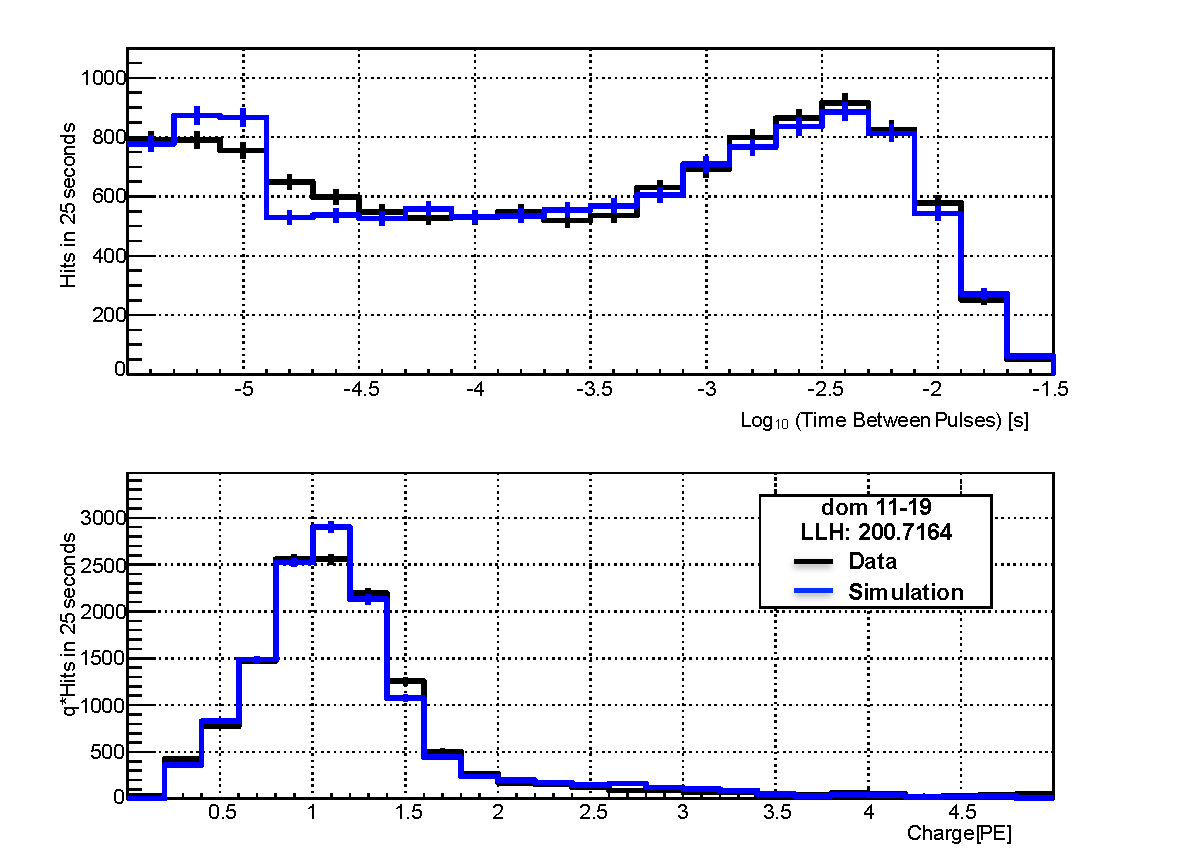
\includegraphics[width=0.45\linewidth]{new_dom_11-19.pdf} \\
  \small (\textbf{\color{ctcolormain}a}) DOM 11-19
\end{tabular} \hspace{2pt}
\begin{tabular}[b]{c}
  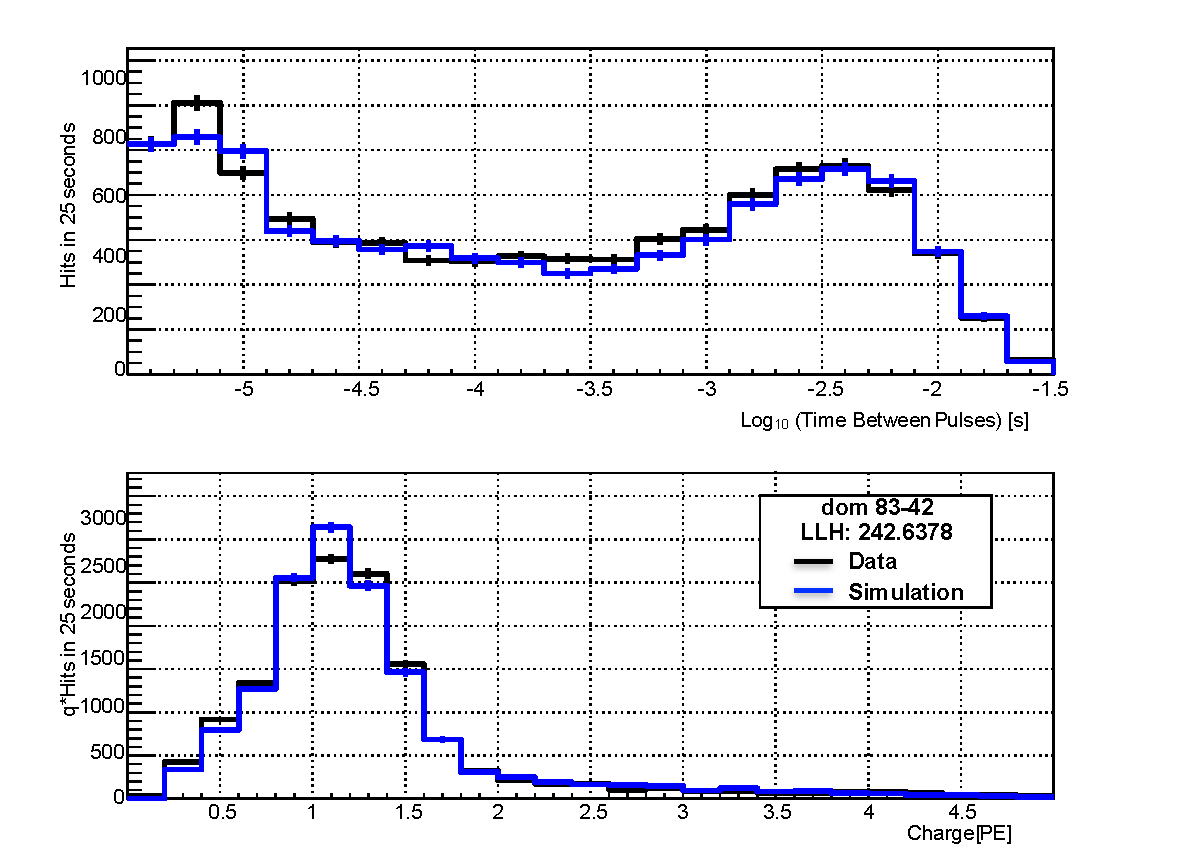
\includegraphics[width=0.45\linewidth]{new_dom_83-42.pdf} \\
  \small (\textbf{\color{ctcolormain}b}) DOM 83-42
\end{tabular}
\caption{Two examples of the new calibration fits for the Vuvuzela V2 model. The distribution of the time ("dt") between hits is shown on top. The distribution of charge is shown on the bottom. Note the y-axis of the charge distribution. In black, untriggered detector data is shown. The Vuvuzela V2 model is shown in blue. The new fits shown good agreement in both time and charge distributions.}
\label{fig:new_vuvuzela_fits}
\end{figure}

The range of the histograms, from 6 microseconds until 1 second in the time and 0-5 photoelectrons in charge, provides sensitivity to the full range of the noise distribution.
The distributions for DOMs 11-19 and 83-42 are shown in Figure~\ref{fig:new_vuvuzela_fits}.

Using the two distributions, a Poisson binned likelihood is formed.
With the simulation in bin $i$ of histogram $j$ denoted by $f_{ji}$ and the data hits in the same bin denoted by $d_{ji}$ and ignoring normalization constants, the log-likelihood takes the form

\begin{equation}
	LLH = \sum_j \sum_i^{\mathtt{nbins}_j} d_{ji} \mathtt{Log}(f_{ji}) + f_{ji}
\end{equation}

The negative log-likelihood, $-LLH$ is minimized as a function of the fit parameters using iMinuit, a python wrapper for the minuit2 package \cite{iminuit-code, iminuit-paper}.

High charges from noise hits were rarely produced, limiting the effectiveness of the fitting strategy.
To provide more weight to high charges, the histogram of the charges was weighted by the value of the observed charge.
This reduces the weight of very low charge launches, but increases the weight of higher charges.

Additional work showed that the charge distributions between data and simulation demonstrated disagreement in the charge distributions. 
This disagreement, due to miscalibration of the SPE peak in data, was accounted for by introducing a scale factor applied to the charge in simulation as a free parameter in the fit.
The charge scaling applied to the simulated hits after detector simulation.
To limit the computational complexity of the added parameter, the minimization over this charge scale factor is performed independently without resimulation.
The form of this charge scale parameter assumes that the difference is a calibration issue in the data rather than a simulation problem.
This has been shown to be the case, with an updated charge calibration now applied to data at final level.

The previous calibration attempts explicitly avoided fitting the behavior below 10 microseconds.
In particular, it was noted that mismodeled afterpulsing behavior could lead to biased results in the noise parameters.
The default value in simulation, assumed to be 5.93\% for all PMTs, failed to take into account variations in the effects on each individual DOM.
In the updated fit, the afterpulsing behavior has been investigated for each PMT by including an overall scale factor on the afterpulsing probability.

Late pulses, produced by electrons which backscatter to previous dynodes during the multiplication process, were also investigated for their effect on the goodness-of-fit in the noise distributions.
These pulses occur at timescales of 50-200 nanoseconds and therefore are outside of both the SLC charge and timing distribution window.
The late pulsing behavior was found to have a negligible impact due to both the rarity of late pulses as well as the lack of detailed information to constrain the distribution.

The effect of the afterpulsing parameter allowed some fits to fall into a poor local minimum. 
The degeneracy between parameters led to a local mimina from which the minimizer could not escape.
In these cases, the probability of observing an afterpulse following a photoelectron would be moved from 5.6\% to the unrealistically high value of 20\%. 
This forced the gaussian mean of the Vuvuzela V2 model to move toward higher values and the gaussian sigma value to become unrealistically large.
These fits were discovered by eye when looking at the best fit value of the afterpulsing probability, with a distinct population appearing due to this behavior.
In order to constrain the fit to more realistic values, bounds were added to both the log-normal mean and afterpulsing probability for DOMs where fits showed abnormal behavior. 
DOMs with particularly strong afterpulsing peaks visible by eye in data were discovered.
These DOMs were allowed to fit beyond the new boundary.

Due to the computational power required to produce large amounts of effective livetime at each iteration of the fitting process, a tiered approach was employed.
Initial fits were seeded with the previous noise parameter fit values obtained in 2012.
For these events, a coarse choice of binning both the timing and charge distributions and short effective livetime of just one minute were used.
In addition, a weak tolerance value was used, allowing the minimizer to converge quickly to a reasonable minimum.

When the first tier completes the minimization process, the fit is restarted with a larger effective livetime, more bins, and a stronger tolerance using the best-fit parameters.
The second tier used a 5 minute effective livetime, increasing the simulation time per iteration by a factor of 5.

The third and final tier increased the effective livetime to 10 minutes and again increased the number of bins.
The final tier of minimization was the most computationally intensive and required between three and four weeks per DOM. 

The fitting process for each tier continued until the minimization either converged or failed.
Failure could occur due to electronics issues, such as computing cluster downtime, or due to a limit of 10000 iterations set in the minimizer to prevent issues with maximum processing time available on the computing cluster. 
In the case of a failure, the fitting tier was restarted with a new set of seed values.
The new seed values were selected from a gaussian distribution centered on the previous seed with a width of 5\%. 
The fit was then restarted.
This process was continued until the third tier was complete for all DOMs.

\label{sec:vuvuzela_newfits}
\section{Results of New Noise Fits}
New calibration fits were completed over the course of two months for nearly all DOMs in the IceCube detector.
String 25 and DOMs previously disabled due to malfunction are absent from the untriggered data, taken in 2014, used here and were therefore left unfit.
The parameters for string 25 were selected using the average of all other fits.


\begin{figure}[h]
\centering
\begin{tabular}{cc}
  	 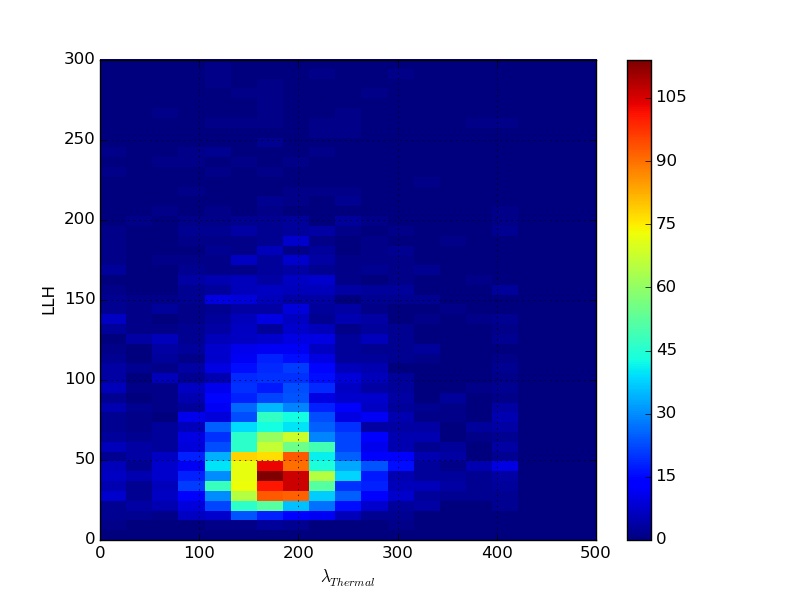
\includegraphics[width=0.45\linewidth]{llh_vs_thermal.png} &
	 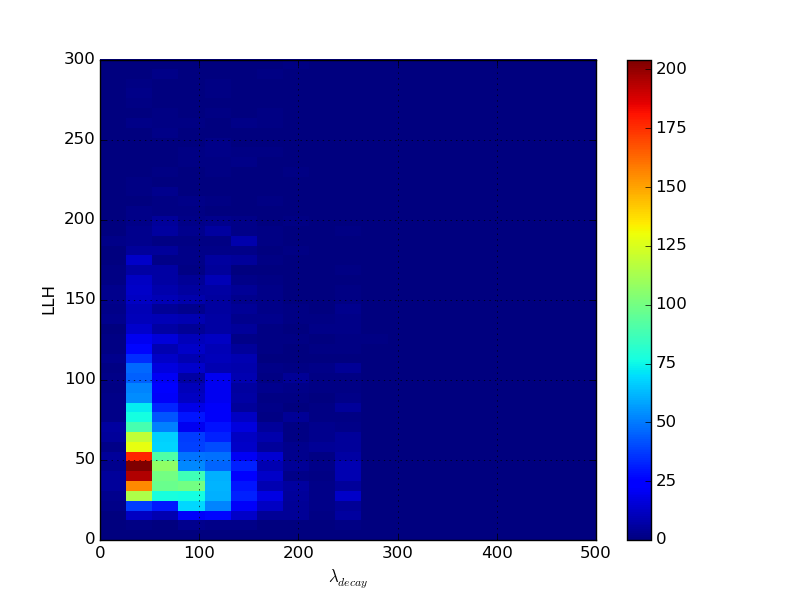
\includegraphics[width=0.45\linewidth]{llh_vs_decay.png} \\
 	 
 	 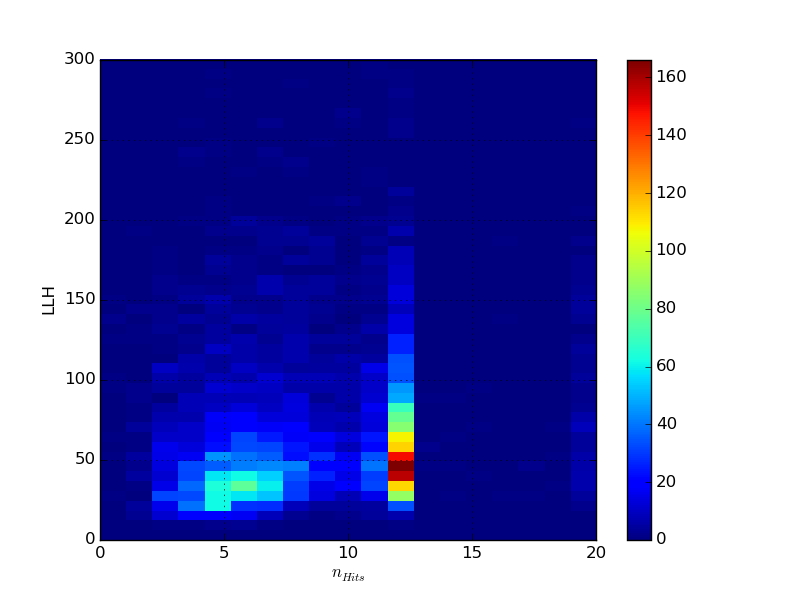
\includegraphics[width=0.45\linewidth]{llh_vs_nhits.png}  &
	 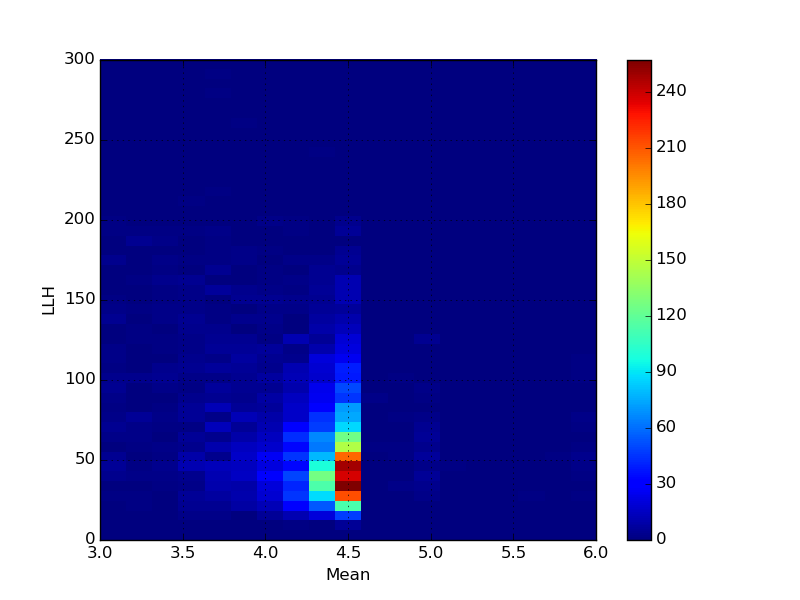
\includegraphics[width=0.45\linewidth]{llh_vs_mean.png} \\

	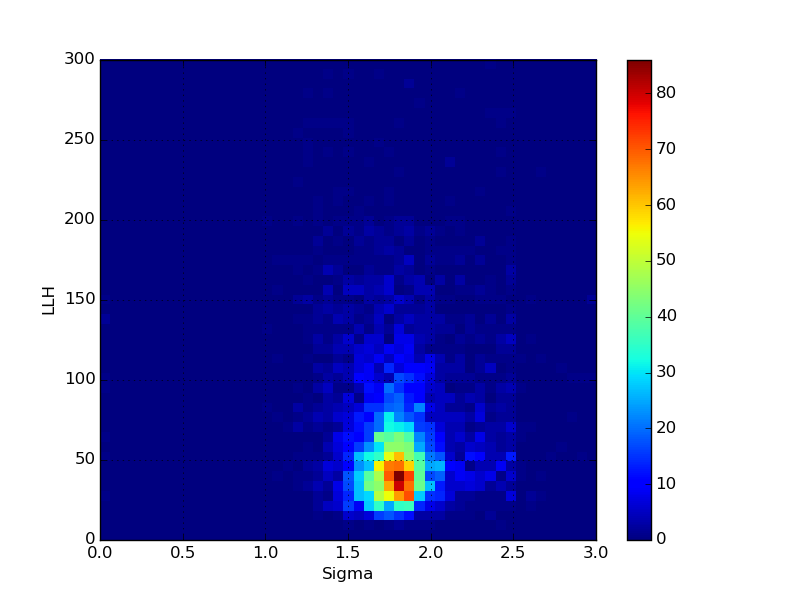
\includegraphics[width=0.45\linewidth]{llh_vs_sigma.png}  &
	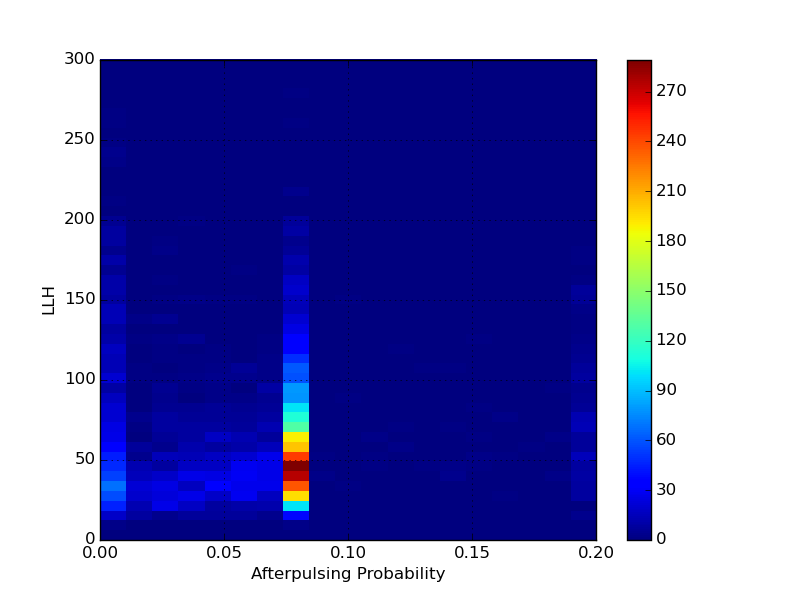
\includegraphics[width=0.45\linewidth]{llh_vs_afterpulsing.png} \\
\end{tabular}
\caption{The distributions of each new fit parameter in the Vuvuzela V2 model. The colorbar scale shows the number of DOMs in each bin. The effects of fit bounds are visible in most distributions except for the thermal noise rate and the width of the log-normal distribution describing the non-Poissonian noise.}
\label{fig:vuvuzela_params_vs_llh}
\end{figure}

The Vuvuzela V2 fits were checked after convergence in Figure~\ref{fig:vuvuzela_params_vs_llh} and Figure.
One notable feature is the number of DOMs with afterpulsing at and beyond the fitter boundary.
The likelihood values associated with these fits, however, appear to be consistent with other fits.
Due to a planned overhaul of the afterpulsing simulation, the fit values of the afterpulsing probabilities have not been adopted for simulation.
Therefore, no further investigation of the probabilities has been persued.

\begin{figure}[h]
\centering
\begin{tabular}{cc}
  	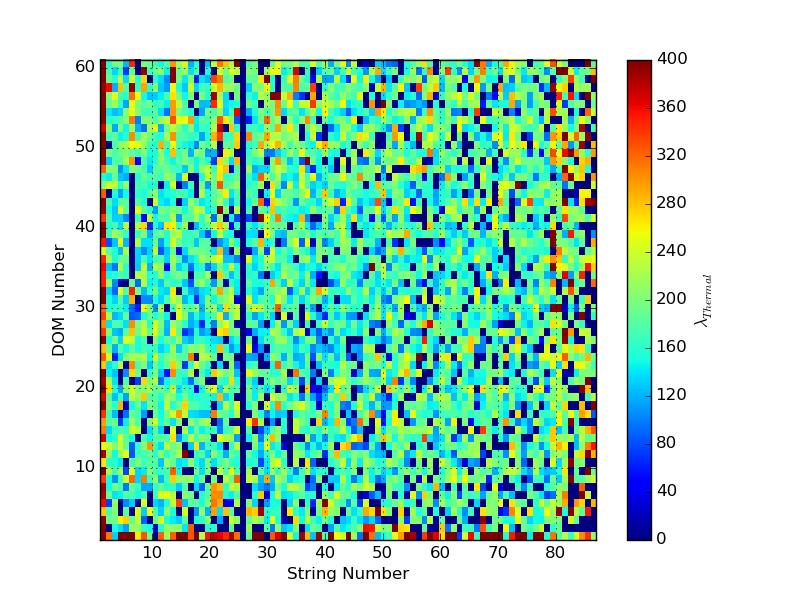
\includegraphics[width=0.45\linewidth]{thermal_occupancy.png} &
	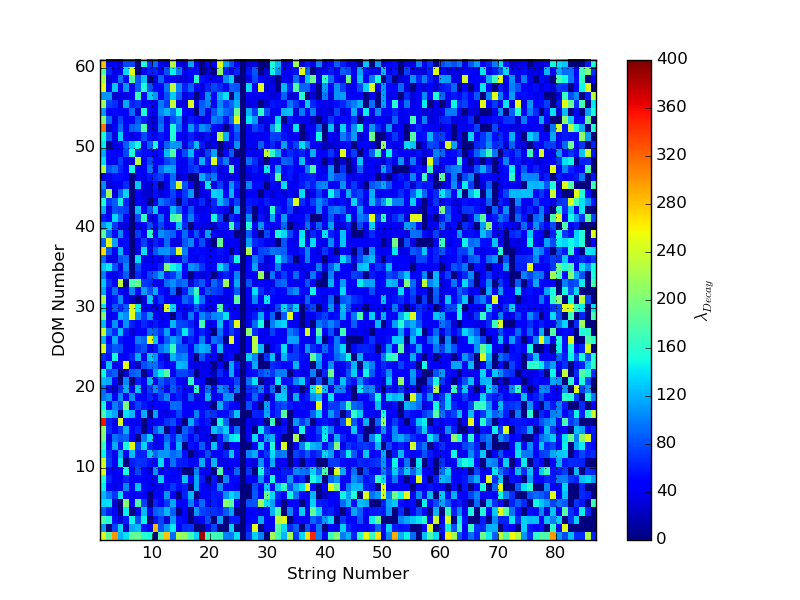
\includegraphics[width=0.45\linewidth]{decay_occupancy.png} \\

  	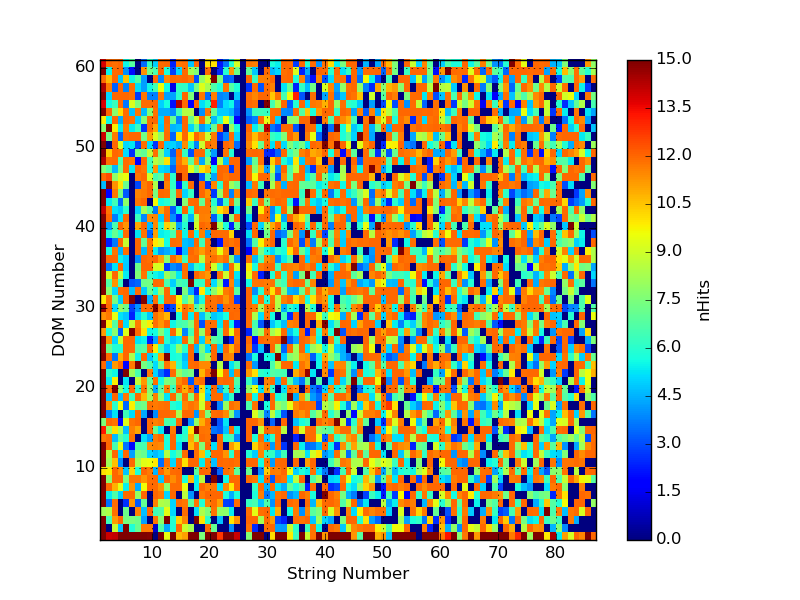
\includegraphics[width=0.45\linewidth]{nhits_occupancy.png} &
	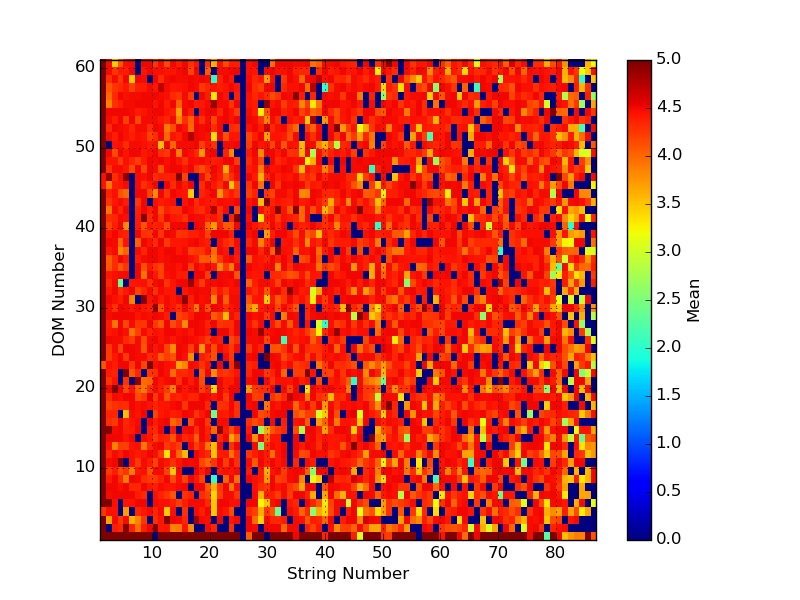
\includegraphics[width=0.45\linewidth]{mean_occupancy.png} \\

  	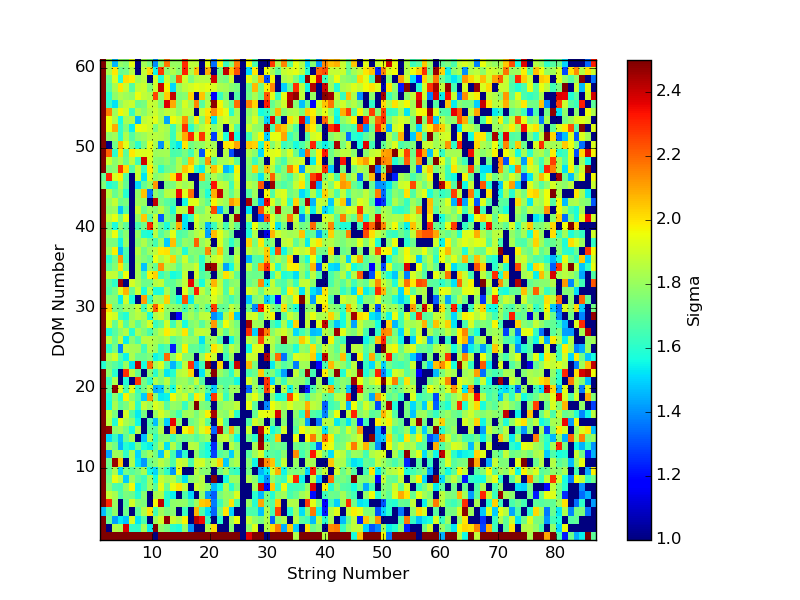
\includegraphics[width=0.45\linewidth]{sigma_occupancy.png} & 
  	\\
\end{tabular}	
\caption{The distributions of each new fit parameter in the Vuvuzela V2 model as a function of the string and DOM number. Note that the top of the detector is at the bottom of this plot. No parameter appears to be correlated with depth. DOMs on string 25 are missing from the dataset. In addition, DOMs which are disabled due to malfunction are also unavailable.}
\label{fig:vuvuzela_params_occupancy}
\end{figure}

The thermal rate is associated with the electronic noise, which should show increasing rate with increasing depth due to the rising temperature.
This effect is only weakly apparent in Figure~\ref{fig:vuvuzela_params_occupancy}.

Other parameters should be independent of depth.
As a test of the fits, each of the other parameters is plotted as a function of depth as well.
No significant correlation is observed.

\begin{figure}
\centering
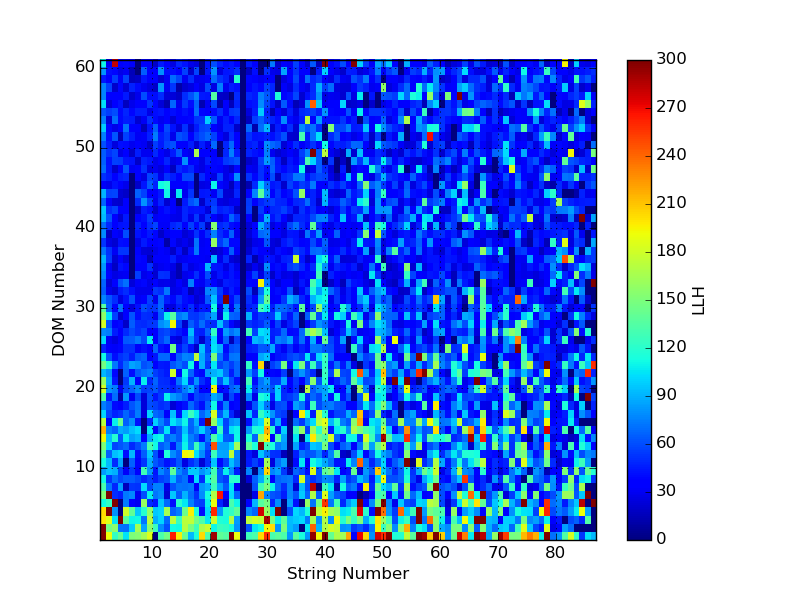
\includegraphics[width=0.9\textwidth]{llh.png} 
\caption{The log-likelihood as a function of string and DOM number for the Vuvuzela V2 fits. Note that DOM 1 is at the top of the detector and DOM 60 at the bottom. The likelihood value was expected to be independent of depth, but shows some structure. These structures are correlated with both the ice model and the muon flux.}
\label{fig:llh_vs_depth}
\end{figure}

Finally, the likelihood values should be independent of depth.
This final test, shown in Figure~\ref{fig:llh_vs_depth},  shows surprising results in at least two ways:
a 'band' structure appears in the plot. and there appears to be a depth-dependent decrease in the likelihood value, indicating that the lower part of the detector yields better fit results.
This was initially unexpected, given that the noise is an internal property of the DOM and not of the surrounding medium.

This effect occurs due to a combination of factors. 
It is worth noting that the noise measurements of each DOM are not fully independent.
The fits themselves use the long-frame CORSIKA to model the effects of muons in the untriggered data from the detector.

This leads to two subtle limitations in the fitting process.
The long-frame CORSIKA is produced with a single flux model, in this case the Polygonato model used in CORSIKA \cite{Hoerandel-Polygonato}.
Because the long-frame CORSIKA cannot be reweighted to other models, uncertainties or mismodeling in the muon flux can lead to disagreement in the fitting of noise parameters.
The muon flux decreases with increasing depth, resulting in a lower muon contamination, and consequently smaller effects from mismodeling of the muon background, for deeper DOMs. 

In addition, the long-frame CORSIKA implicitly assumes a single model of the ice for photon propagation.
Mismodeling of the scattering and absorption of the ice therefore may also give rise to disagreement in the noise calibration.
While large-scale properties of the ice are believed to be well-reproduced by the chosen ice model, SpiceLea \cite{IceCube-SpiceLea}, there will inevitably be remaining disagreements.

The net effect of these two assumptions in the muon simulation is effectively correlated with the convolution of the ice model and the muon flux.
In particular, the best fits occur where the DOM is either A) well-shielded from light due to muons by the large overburden or B) well-shielded due to large absorption in the ice.
In both cases, the contamination from light due to muons in the fitted time and charge distributions will be small, leading to a more 'pure' noise distribution that is well-fit by the Vuvuzela V2 noise model.

The sensitivity of the noise calibration procedure to underlying assumptions of both the muon flux and the absorption properties in the detector imply that little further improvement is likely without additional work on one or both issues.
Simulation of long-frame CORSIKA is, unfortunately, not possible with newer flux models at this time.
As the primary uncertainty affecting the goodness-of-fit appears to be due to the visibility and flux of the muons themselves, merely updating to a newer model of the ice will be unlikely to significantly improve the current fit parameters.

The newly calibrated low-dt Vuvuzela was provided to the IceCube simulation group in January of 2015 and quickly integrated into the low-energy simulation chain.
New neutrino, muon, and accidental noise trigger simulations were produced soon thereafter.
The updated noise model shows significantly better agreement in both the total charge distribution and the number of hit DOMs for both HLC and SLC+HLC hits.
The rate of accidental triggers improved relative to previous calibrations, with the remaining rate disagreement reduced from 50\% to approximately 15\%.
Negligible effect was observed in the low-energy neutrino events at final level for existing samples.



\label{chapter:muonsim}
\chapter{Low-Energy Muon Simulation}

\label{sec:longframe_corsika}
\section{Long-Frame CORSIKA for DeepCore}
One of the primary difficulties for low energy analyses in IceCube is the modeling of backgrounds.
Two significant backgrounds exist for a standard muon neutrino disappearance measurement: the events due to cosmic-ray induced muons and the events from accidental triggers in the detector due to random detector noise.

The two types of simulation are somewhat interdependent.
In particular, the accidental trigger rate, defined to include only events in a trigger is primarily caused by noise hits, relies on the rate of atmospheric muons to calculate an effective livetime for possible noise triggering.
In turn, the atmospheric muon triggering and filtering rate depends somewhat on the characteristics of the noise model used in the simulation.

At the lowest energies, the interplay between atmospheric muons and noise becomes more muddled.
The falling muon spectrum ensures that there are a significant number of muons that potentially reach the IceCube detector even down to cosmic ray primary energies of approximately 600 GeV, where the overburden from the glacial ice yields a natural cutoff to the specrum.
At these energies, a shift in either the muon rate or the noise rate can change the hit rates at the top of the detector.
These low-brightness muons are largely indistinguishable from noise hits, but are not simulated using the Vuvuzela module.
Ignoring these muons can result in a systematic mismodeling of the detector background that changes as a function of depth, with the worst agreement at the top of IceCube.
These muons, called \textbf{sub-threshold muons}, have been shown to be responsible for a significant fraction of hits in the detector \cite{heereman_thesis}.

While the 5-component CORSIKA described in \ref{subsubsec:corsika} generally gives much more freedom to fit and correct for spectral characteristics, the events cannot easily produce the low-energy muon background characteristics at the top of the detector.
Instead, the most accurate way to model these effects relies on long-frame simulation described in \ref{subsubsec:noise_triggers}. 
These frames, consisting of a continuous detector simulation over the course of tens of milliseconds or longer, can be combined with CORSIKA simulation in order to produce the most accurate background simulation possible with current tools.

Long-frame CORSIKA generally requires a modeling of a natural flux of events in the detector.
Given the currently available toolset, only the polygonato mode of the CORSIKA generator is therefore able to be used for long-frame generation.
While there are currently ideas for how to generate with a more acccurate spectral model, they prove to be inefficient without a reparametrization of the generation from the CORSIKA code itself and will not be discussed here.

To produce long-frame CORSIKA simulation, a few modifications of the standard simulation scheme are required.
A frame length, $\tau$ is chosen at the start of simulation. 
Longer values of $\tau$ will generally yield more accurate simulation due to issues at the start and end of a frame, although this is a minor concern in practice.
With this time, an expected number of particles may be extracted given a spectrum $\Phi_\mu$ and a simulation volume $V$:

\begin{equation}
	\label{eq:n_{expected}}
	\bar{N_{\mu}} = \int_{t=0}^{\tau} \int_E \int_\Omega \int_V \Phi_\mu
\end{equation}

This is an analytic formula, yielding the poissonian expectation on the expected number of muons in the simulation volume.
A number of muons is then calculated as a poisson-fluctuation of this number.
The CORSIKA generator will produce the requested number of muons in this time frame.
These muons can be either single muons or occur as muon bundles.
In the latter case, the entire bundle is treated as a 'muon' for the purposes of this section.

The muons are evenly distributed throughout the simulation window following the assumption that each muon is independent of all others (ie, that they are not due to the same cosmic ray interaction in the atmosphere).
From this point, the long-frame simulation scheme described in \ref{subsubsec:noise_triggers} continues, with detector simulation and splitting occuring in the CoincidenceAfterProcessing module.

Long-frame CORSIKA simulation is a useful tool for low energy analyses, yielding a collection of accidental trigger events and muons that would otherwise be produced separately and require reweighting.
In addition, emergent properties of the subthreshold muons are included in these simulation sets.
Unfortunately, the production of long-frame CORSIKA simulation is particularly computationally expensive and of limited use for most higher energy analyses ongoing in the IceCube collaboration.
Very little long-frame CORSIKA simulation is therefore available.

For this work, long-frame CORSIKA simulation was crated with an effective livetime of approximately two weeks. 
Such a sample required months of simulation time, severely limiting the potential usefulness for analyses.
Still, the existing sets proved useful and necessary for the work in \ref{chapter:vuvuzela}. 
Furthermore, the sets provided the first background estimates for both accidental triggers and atmospheric muons for the PINGU/Phase 1 detector described in \ref{chapter:pingu}.

Initial tests with the long-frame CORSIKA simulation showed, for the first time, notable disagreement in the charge distributions in data and simulation described further in \ref{sec:vuvuzela_limitations}.


\label{sec:muongun_deepcore}
\section{MuonGun for DeepCore}



\label{sec:kde_filtering}
\section{Simulation Efficiency with KDE Filtering}
The production of background atmospheric muons is the most computationally expensive part of oscillation analyses in IceCube. 
For the primary analysis of this thesis, full CORSIKA simulations have proven to be impractical. 
When simulating at the detector threshold, many of the produced showers lead to no significant contribution to the detector output, leading to significant inefficiency.
In addition, the choice of cuts employed (see \ref{chapter:greco}) lead to a low simulation efficiency at final level that has both strong energy and zenith dependences.

For this work, a set of $3\times 10^{9}$ muons were produced using collaboration resources over a period of approximately three months.
Muons were produced following the MuonGun scheme described in \ref{subsubsec:muongun}, with all muons aimed toward the DeepCore fiducial volume.
The resulting generation-level distributions are shown in \ref{fig:mg_generation}.
The muons follow the offset power law described in \ref{subsubsec:muongun} in energy and the expected zenith angle spectrum from the underlying flux model of \cite{h4a}.
The generated muons show azimuthal symmetry as expected.

After processing to the final level of the GRECO event selection (see \ref{chapter:greco}, the background muon simulation retains approximately 9000 simulated events of the original sample.
This remaining subsample may be used to estimate the simulation efficiency of muons in this selection.
The efficiency is most easily observed with low energy muons that travel very downgoing, as seen in \ref{fig:mg_ineff}.
These events make up the majority of simulated muons at generation level, but no such events reach the final level of the analysis.

In addition to the energy- and zenith-dependent effects, the GRECO selection exhibits strong azimuthal selection bias.
This arises due to two main effects. 
The first is the offset between the center of IceCube (and therefore the center of the generation volume) at $(x,y,z)=(0,0,0)$ and DeepCore at $(x,y,z)=(XXXXXXX)$.
This gives rise to an azimuthal effect appearing as a sinusoidal variation of the minimum generated energy of events at final level.

The second is the regular hexagonal structure of the IceCube volume, with long "corridors" through which muons may reach DeepCore without crossing any strings.
Cuts designed to look for hits left in the veto region produce these azimuthal biases when muons close to strings (ie, outside of the "corridors") are more likely to be identified and removed than those further from strings (inside of the "corridors").

In order to improve simulation statistics at final level, the existing MuonGun simulation scheme was modified to include an energy-, zenith-, and azimuthally-dependent prescale factor.
This approach, here entitled \textbf{KDE Filtering}, allows simulation to be produced with a known bias matching that of a given set of input files.

In this scheme, the \textbf{kernal density estimator} (\textbf{KDE}) from SciPy \cite{scipy} is applied to all remaining events at final level of the GRECO event selection. 
The KDE uses a Gaussian kernal to represent each event in energy, zenith, and azimuth. 
The resulting KDE is normalized to produce an approximation of the final selection probability density function.

In the new simulation scheme, an event is produced using standard settings for MuonGun generation. 
Immediately following generation, the probability of the new event reaching final level is calculated from the KDE, with typical values 
of approximately $10^{-4}$ for a likely event and $10^{-9}$ or lower for unlikely events.
A prescale multiplicative factor of $10^5$ is used to set the overall probability scale.
The product, $p$ of the prescale factor and KDE-derived probability may not exceed 100\% and any values for which this may be the case are directly set to 100\%.

Using a random number generator, this $p$ factor is used to retain or reject the muon event.
The simulation then proceeds as normal, with photon propagation, detector simulation, triggering, and filtering.

When events need to be weighted by a flux model, the $p$ factor must be included as well. 
The modification to the weighting scheme requires the use of the original MuonGun weighting code in the usual scheme. 
The total weight is then scaled by $\frac{1}/{p}$, which corrects the rates and uncertainties for the simulated events.

By removing unlikely events early in the simulation chain, the required computational resources are significantly reduced.
In addition, the updated simulation scheme gives the opportunity, for the first time, to study various detector systematics affecting the atmospheric muons at the final level of oscillation analyses.

By way of comparison, the total amount of time required to produce 9000 events at final level of the GRECO selection with similar available resources reduces from three months under the standard scheme to approximately four days using the KDE filtering method.




\label{chapter:greco}
\chapter{GRECO: An Event Selection at the Limits of DeepCore}

\label{sec:level3}
\section{Low-En Level 3 Cuts}

\label{sec:level4}
\graphicspath{{chapters/greco/images/level4/}}

\subsection{GRECO Level 4 Cuts}
The first GRECO-specific cut level, designated \textbf{level 4}, or \textbf{L4}, was first introduced in 2011 using variables common to higher energy cascade analyses within IceCube. 

At the start of this series of cuts is requirement of at least three hit DOMs in the hit series associated with an event. 
This is an extremely loose cut, required solely for the successful processing of other cuts.

The remaining cuts at L4 can be divided into two groups: those that rely on a rough reconstruction of the event and those that are based solely on charge deposition.

\subsubsection{FirstHit Z}
\begin{figure}[h]
	\centering
		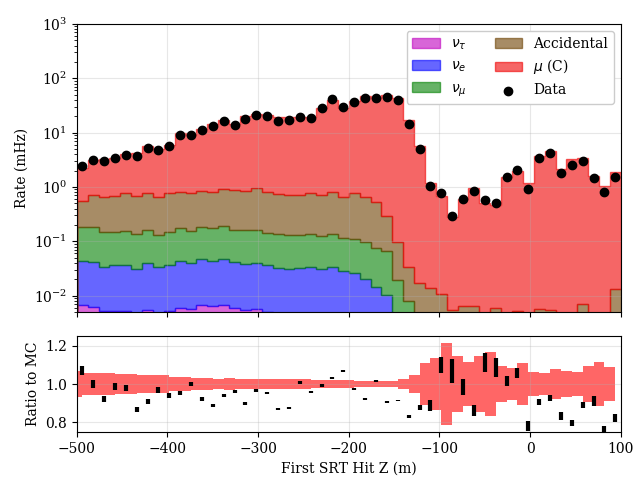
\includegraphics[width=2.5in]{FirstHitZ_log.png}
		\caption[The FirstHit Z position]{The Z position of the first hit in a cleaned hit series. Note the shape difference between the atmospheric muons in red and the various neutrino flavors, particularly above -200 meters.}
	\label{fig:firsthitz_log}
\end{figure}

Muons generated in the upper atmosphere through cosmic ray air showers will generally be visible as they enter the detector. 
As they pass through the veto layers, the muons may emit light via Cherenkov emission or via stochastic processes. 
This light leaves a signature behind in the detector in the form of hits along the true muon track. 

Because the muon tracks are primarily steeply inclined, most will leave hits in the upper part of the detector.
Neutrinos, on the other hand, will emit light following an interaction.
For the low-energy neutrinos of interest to this analysis, interactions will occur primarily in the DeepCore fiducial region, leading to little or no light emission in the top half of the detector. 
This difference between neutrino and muon emission in the upper part of the detector can be used to identify background muons with little additional processing.
For this analysis, the first hit in a cleaned hit series, the time-window cleaned DeepCore pulses, is called the \textbf{FirstHit Z} in the Level 4 cuts.

\subsubsection{NAbove200}
\begin{figure}[h]
	\centering
		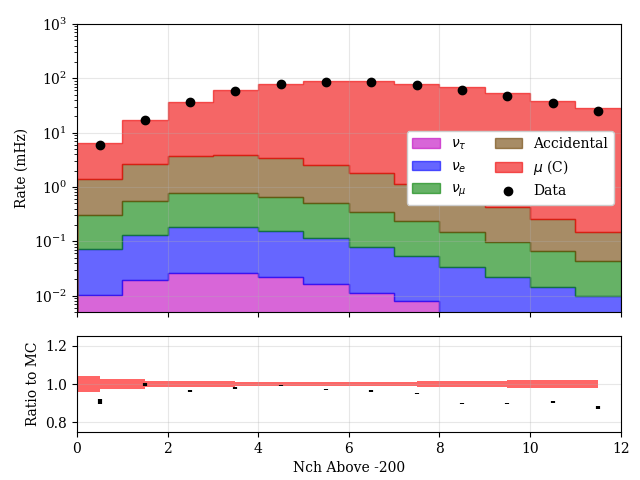
\includegraphics[width=2.5in]{NAbove200_log.png}
		\caption[Number of Hits Above Z=-200]{The number of hits above Z=-200 meters}
	\label{fig:nabove200_log}
\end{figure}

The position of the first hit in DeepCore is not the only low-level cut to arise from the emissions of the muon and neutrinos. 
The total charge of recorded hits occuring in the top of the detector is also used in the analysis. 
This variable, known as \textbf{NAbove200}, counts the amount of charge occuring before the SMT3 trigger above a depth of -200 meters.

\subsubsection{QR6/C2QR6}
\begin{figure}{h}%
	\centering
		\subfloat[QR6]{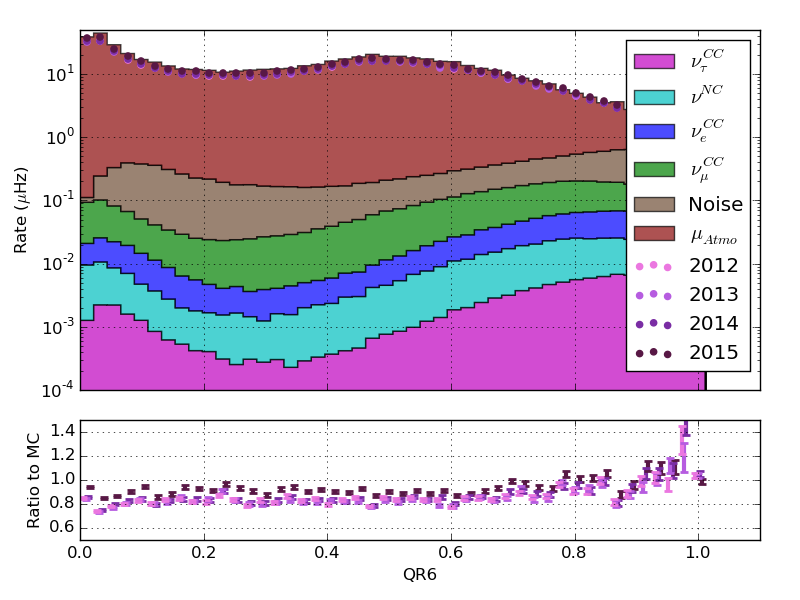
\includegraphics[width=2.3in]{QR6_log.png}}%
		\subfloat[C2QR6]{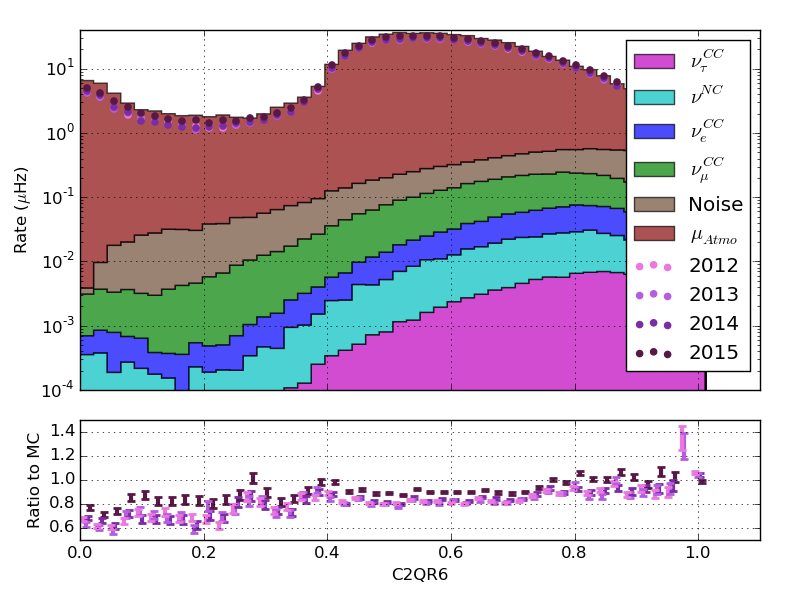
\includegraphics[width=2.3in]{C2QR6_log.png}}%
	\caption[QR6 and C2QR6]{The charge ratio variables used in the L4 cuts.}%
	\label{fig:QR6_and_C2QR6}%
\end{figure}

After a particle interacts, the light emission as a function of time will depend on the type of particle emitting.
A very basic model of cascade-like events assumes that photons are emitted roughly instantaneously from a point-like source at the interaction vertex. 
The photons then travel outward according to a random walk with absorption, leading to a decay in the observed number of photons over time.
A muon, however, acts as an extended source and will emit at multiple points along the muon track until it either falls below the Cherenkov threshold or is stopped.

The light emission is, therefore, more likely to be "peaked" in time for neutrinos than for muons. 
Using this information, two variables are designed to seach for this peakedness in the light detection over time.

The first of these, the \textbf{charge-ratio within 600 ns} (hereafter \textbf{QR6}), is the ratio of the charge occuring within 600 ns of the first hit compared to the total charge of the event.
The value of 600 ns was chosen in a previous analysis and is not re-optimized here.
Regardless, this time corresponds to roughly two ATWD time windows or approximately 180 meters at the speed of light in vacuum.
This distance, which will correspond to a wide swath of the DeepCore fiducial volume, provides some separation between muons and neutrinos.

\subsubsection{QR6 plot}

Neutrinos and muons do not produce the only hits observed in the detector, however. 
Random detector noise, in particular, can significantly change the choice of time used.
In order to check the effect of random noise contributing the first few hits of the event, a second variable, known as \textbf{C2QR6}, is introduced.
This variable is calculated in an identical way to QR6, but the first two observed hits are ignored.

\textbf{C2QR6 plot}


\subsubsection{Tensor of Inertia}
\begin{figure}[h]
	\centering
		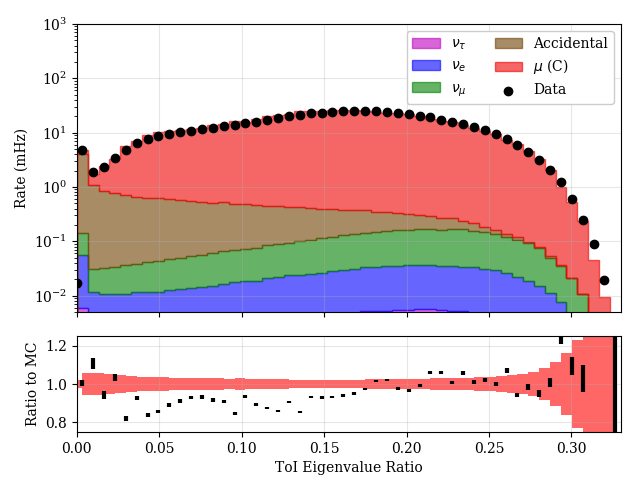
\includegraphics[width=2.5in]{ToIEval_log.png}
		\caption[Tensor-of-Inertia Eigenvalue Ratio]{The eigenvalue ratio from a ToI calculation. Larger values indicate more apparent elongation in the event.}
	\label{fig:toi_log}
\end{figure}

At this early level, the shape difference in the observed hit pattern will be relatively clear.
Neutrinos with energies in the range of 1-100 GeV will appear to be rather small and compact, while muons will have a longer extent in one direction along the muon track than perpendicular to it.
In order to utilize the shape differences between these two types of particles, the \textbf{Tensor of Inertia eigenvalue ratio} (more briefly, \textbf{ToI}) is used.
This variable is defined in a similar way to the tensor of inertia from mechanics, with the measured charge taking the place of the mass.

\begin{eqnarray}
	I_{X} = \sum_{i=0}^{nhits}(y_i^2 + z_i^2)q_i	
	I_{Y} = \sum_{i=0}^{nhits}(x_i^2 + z_i^2)q_i
	I_{Z} = \sum_{i=0}^{nhits}(x_i^2 + y_i^2)q_i
\end{eqnarray}

These three moments yield information about the shape of the event.
The eigenvalue ratio is defined as 

\begin{equation}
	e = \frac{\mathtt{max}_j(I_j)}{I_{x}+I_{y}+I_{z}}
\end{equation}


\subsubsection{Improved Linefit Speed}
\begin{figure}[h]
	\centering
		\includegraphics[width=2.5in]{iLineFit_Log.png}
		\caption[The improvedLineFit Speed]{The apparent speed, in units of meters per nanosecond, corresponding to the hits in the event. Faster speeds are associated with particle travel instead of light travel.}
	\label{fig:ilinefit_log}
\end{figure}



\subsubsection{The L4 BDT}
\begin{figure}[h]
	\centering
		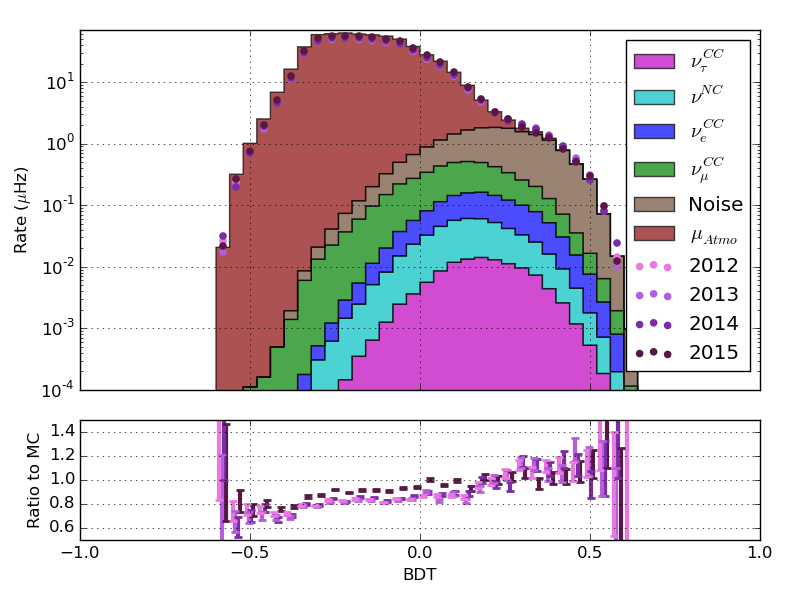
\includegraphics[width=4in]{BDT_log.png}
		\caption[The L4 BDT Score]{The distribution of the boosted decision tree used at L4. A cut is applied at 0.04 to remove a significant fraction of atmospheric muon background events. Note the ratio, which shows disagreement in the very muon-like region. The region of disagreement is removed by the cut.}
	\label{fig:L4_bdt_log}
\end{figure}

A Boosted Decision Tree (\textbf{BDT}) is trained at L4 to further reduce the atmospheric muon background by a factor of 10x. 

The variables described above were provided to a BDT training using the CORSIKA 7437 and IceSim3 GENIE simulation. 

Burn sample distributions match in the years 2012/3/4/5, but are notably different for 2011. 
I believe the reason is related to the deployment: once new DOMs are deployed, they take 1-2 years to completely cool down 2011 is therefore excluded for this analysis.

Comparisons to MC show mild disagreement, particularly in the most muon-like regions that get cut away. 
Its not obvious what is the cause of the disagreement, although its possible that the assumed cosmic ray flux model (H4a) is simply an inaccurate model of some part of the spectrum that contributes. 
This may be particularly true, since H3a and H4a contain different compositions at high energies. 
These differences would contribute to different parts of the atmospheric muon spectrum at the detector, where the highest energy atmospheric interactions leading to visible muons will occur at the horizon. 
If these (or other systematics on the CR/muon spectra) give rise to different HE muon distributions, those muons would appear to have clear tracks and would show up on the far left of the BDT distribution.

In the right side of the plot, a shoulder attributable to the noise triggers is visible. 
While this is initially surprising, the reason for this is obvious: the BDT was originally trained with CORSIKA set 7437 and weighted GENIE sets.
Both cases had incorrect modeling of the detector. 
Both had DOM oversizing applied and DOM efficiency set to 0.9 (the old nominal value) instead of the 0.99 that we now use. 
The training itself lacked any pure noise triggers as a reference, and so the BDT picked the most obvious feature of the GENIE sets: that the signal events were primarily low energy with lower light deposition than the background. 
These are also key features of the noise triggers. 


\label{sec:level5}
\graphicspath{{chapters/greco/images/level5/}}

\subsection{GRECO Level 5 Cuts}
The next stage of cuts, know as the \textbf{GRECO Level 5}, or more simply, \textbf{L5}, is structured in a similar manner. 
Once again, there exists both a relatively simple cut dedicated to removing accidental triggers due to noise as well as a BDT consisting of six variables.

\subsubsection{L5 Straight Cuts}
The former is a again cut on the number of hits similar to the cleaning applied in the L3 cuts. 
This time, however, a slightly different cleaning is applied, consisting of both a static and a dynamic time window applied to the split DeepCore pulses.
The static window, with a width of 7500 nanoseconds, removes hits that are far from the trigger in order to limit the effect of random detector noise.
The dynamic time window is designed to specifically look for a set of hits spaced very closely in time.
For the L5 noise trigger cut, a dynamic window is chosen of 200 nanoseconds.

After the two time window cleaning algorithms are applied, the resulting hit series is required to posses at least 3 remaining hits to be accepted for further processing.

\subsubsection{Time to 75\% Charge}
\begin{figure}[h]
	\centering
		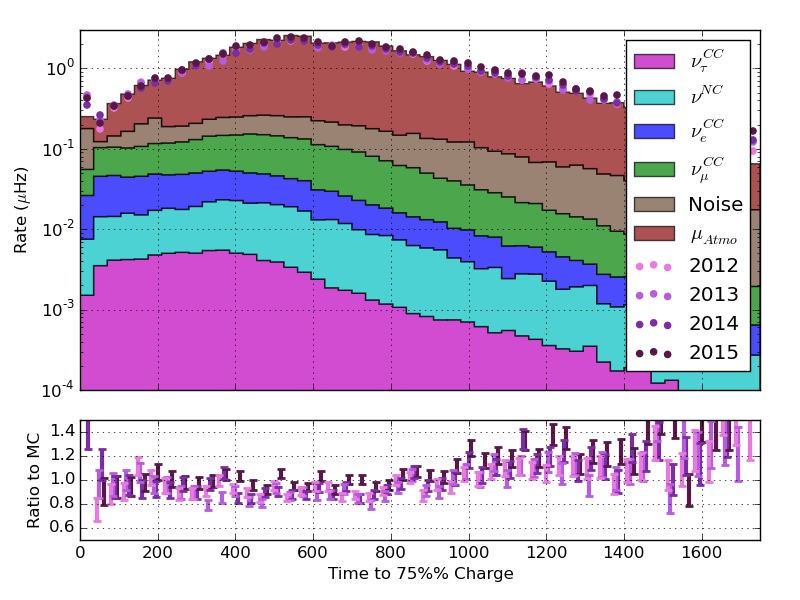
\includegraphics[width=2.5in]{Time_to_75_Charge_log.png}
		\caption[Time to 75\% Charge]{The time to accumulate 75\% of the total charge of the event.}
	\label{fig:time_to_75}
\end{figure}

The first variable used to create the L5 BDT is the amount of time to accumulate 75\% of the total charge, the \textbf{$t_{75}$}. 
The idea behind this variable is again similar to that of the QR6 and C2QR6 variables and will not be repeated here.
However, the variable is now produced in the reverse manner: where the QR6 variable refers to the amount of a charge in a given window, the $t_{75}$ instead attempts to find the amount of time for a given charge level, providing an additional handle on the total event length and timing distribution.


\subsubsection{Veto Identified Causal Hits}
\begin{figure}[h]
	\centering
		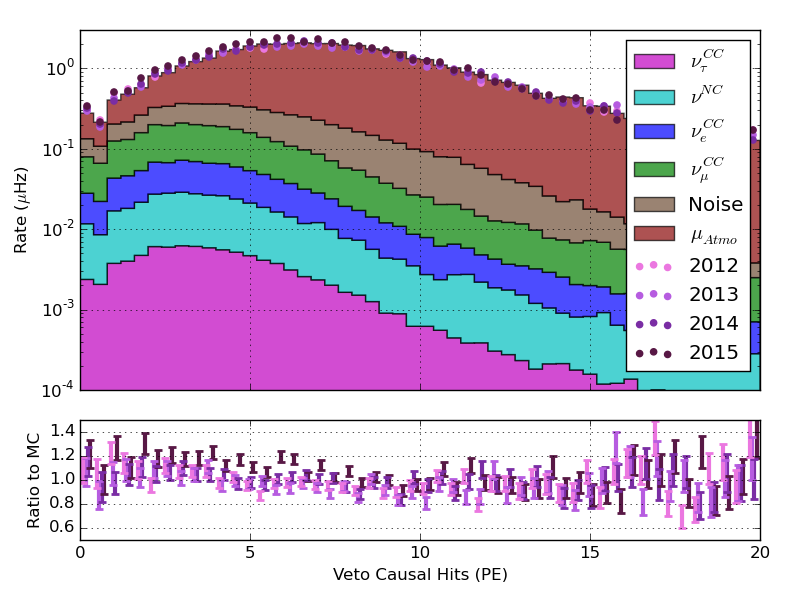
\includegraphics[width=2.5in]{Veto_Causal_Hits_(PE)_log.png}
		\caption[Veto Identified Causal Hits]{The amount of causally-connected charge discovered in the veto region.}
	\label{fig:vich}
\end{figure}

The \textbf{Veto Identified Causal Hits} (\textbf{VICH}) algorithm is a second choise for the L5 cuts that relies solely on low-level charge information.
In this case, we improve on causality constraints using the trigger time and the position of the first DOM to contribute to the trigger.
The time and distance are calculated to each other hit relative to this simplistic event vertex.
Any hits that occur in a window before the trigger that are approximately causally connected to this hit are recorded, with the total charge thus recorded giving the cut variable.
The window is described in \ref{fig:VICH_definition}


\subsubsection{First Hit $\rho$}
\begin{figure}[h]
	\centering
		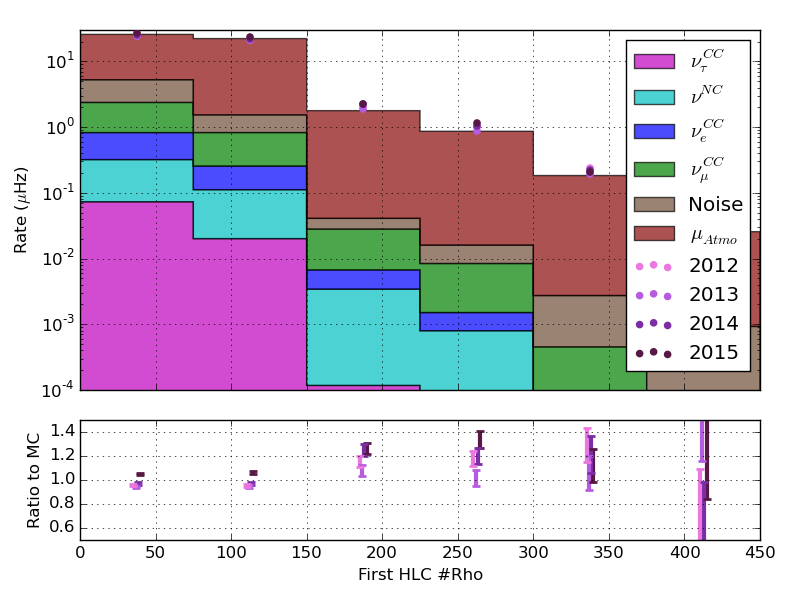
\includegraphics[width=2.5in]{First_HLC_Rho_log.png}
		\caption[First Hit $\rho$ Position]{The radial position of the earliest hit of a cleaned hit series. The radial position is measured relative to string 36, the center of DeepCore.}
	\label{fig:firsthit_rho}
\end{figure}

Further simple event vertices give additional separation power. 
In particular, the radial position of the first hit in a STW cleaned (7500 ns) hit series encompassing solely the DeepCore fiducial volume may be used to identify incoming atmospheric muon events.


\subsubsection{Quartiles CoG}
\begin{figure}[h]
	\centering
		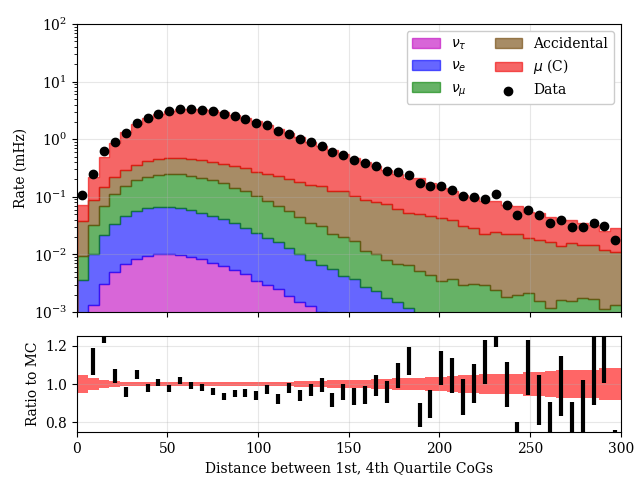
\includegraphics[width=2.5in]{Q1-Q4_Distance_log.png}
		\caption[Quartile Distance]{The distance between the centers of gravity of the first and last quartile in time.}
	\label{fig:quartile_distance}
\end{figure}

The traveling distance of a muon may be exploited in order to identify muons as well.
In particular, a track-like event is expected to travel over a longer distance than a cascade-like event of a similar energy.
Looking at the first and last quartiles in charge, the length of the vector from one of the CoGs to the other can give some simple indiciation of the length of a hypothetical track in the event.

\subsubsection{Z-Travel}
\begin{figure}[h]
	\centering
		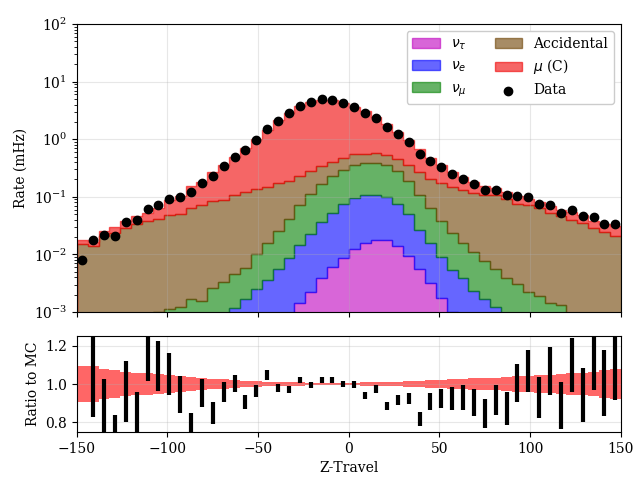
\includegraphics[width=2.5in]{Z-Travel_log.png}
		\caption[Quartile Z-Travel]{The distance traveled in Z between the first and last quartile of hits in time.}
	\label{fig:quartile_ztravel}
\end{figure}

Atmospheric muons are primarily a downgoing feature of the detector, with a flux that approaches zero at the horizon.
Muons will, therefore, leave some information in the depth and directional information collected by the detector.
The first variable to utilize this, \textbf{Z-Travel}, identifies the distance in the z-direction between the first and the last quartile of hits using the CoGs calculated in the previous variable.

\subsubsection{SPE Zenith}
\begin{figure}[h]
	\centering
		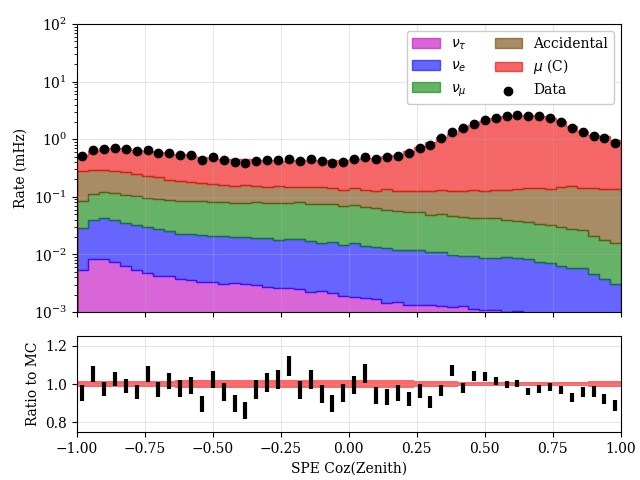
\includegraphics[width=2.5in]{SPE11_Cos(Zenith)_log.png}
		\caption[SPE Reconstruction Zenith Angles]{The zenith angle distribution of events from an 11-iteration SPE fit. The fit assumes an infinite track hypothesis and uses only hit DOMs.}
	\label{fig:spe11_zenith}
\end{figure}

More advanced reconstructions are viable at this level, providing new potential for the identification of atmospheric muons from neutrino candidates.
Using the first pulse on each DOM, a likelihood reconstruction may be produced.
A fast likelihood reconstruction assuming an infinite track passing through the detector with light scattered via the Pandel scattering model of ice is one such tool.

The Pandel model of scattering, while known to be inaccurate, provides an analytic form that is fast to evaluate in order to find the charge expectation as a function of relative position and direction between the hypthesized track and each DOM.
The reconstruction is begins with a seed of some description that my slightly gin-addled mind with no internet access cannot recall.
A total of eleven directions are used as seeds around the seeded position and time, including a seeded direction.
For each hypothesis, the expected charge at different time steps is compared to the observed charge at each DOM using a Poisson binned likelihood.
The best-fit of the eleven reconstructions is returned.

Again, atmospheric muons are primarily downgoing events. 
Therefore the direction of the reconstructed track is a useful tool for separating neutrino signal and atmospheric muon background.


\subsubsection{The L5 BDT}
\begin{figure}[h]
	\centering
		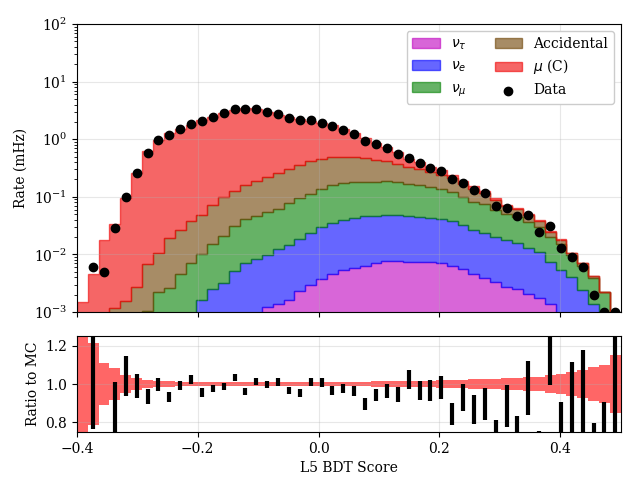
\includegraphics[width=4in]{BDT_Score_log.png}
		\caption[The L5 BDT Score]{The distribution of the boosted decision tree used at L5. A cut is again applied at 0.04 to remove a significant fraction of atmospheric muon background events.}
	\label{fig:L5_bdt_log}
\end{figure}

The six variables described in this section are again used to create a BDT. 
At the time of training, updated versions of both the GENIE and CORSIKA simulations were provided as part of a ongoing upgrade of the IceCube simulation.
In particular, the L5 BDT was trained using simulation files containing the then-newly available Vuvuzela noise model and an updated version of the GENIE Monte Carlo generator.

A set of fifteen variables were tested.
At each step of the training, the least important variable was removed to limit the possible effects of overtraining.
The process continued until changes in the cut efficiency larger than 1\% were observed, resulting in a boost decision tree containing the six most important variables tested as described above.

The distribution of BDT score is shown in \ref{fig:L5BDT_log}. 
The data and simulation show good agreement across the range of scores.
In addition, the distribution of shows some separation from the neutrino events, providing some cut power.

A cut is placed at a score of 0.04, which gives approximately 95\% background rejection with a somewhat significant hit of 30\% to all neutrino rates.






\label{sec:level6}
\graphicspath{{chapters/greco/images/level6/}}

\subsection{GRECO Level 6 Cuts}
Unlike previous levels, the GRECO L6 does not rely on a trained boosted decision tree.
The choice was made to use solely stright cuts due to initial concerns about the significantly limited background simulation.
Such a limitation could lead to overtraining, a situation difficult to test with so few simulated events.

Instead, there are effectively two types of cuts used in the GRECO L6:
those that deal, directory or indirectly, with removing accidental triggers and those that focus on the starting containment of events in the DeepCore fiducial volume.

\subsubsection{Fill-Ratio at L6}
\begin{figure}[h]
	\centering
		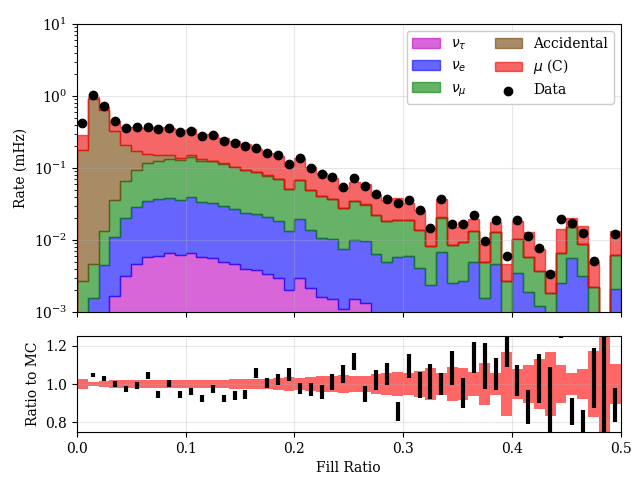
\includegraphics[width=2.5in]{FillRatio.png}
		\caption[Fill-Ratio]{The fill-ratio distribution. Note the excess of noise triggers at low values. A cut is applied at 0.05 to remove these accidental triggers.}
	\label{fig:fill-ratio}
\end{figure}

A continuing thread of the event selection deals with understanding and removing events caused by detector noise triggering in the DeepCore fiducial volume.
While the rate of these accidental triggers is low at this stage relative to the rate at L3, they form an important background to the remaining set of neutrino events.
In order to limit their effect, various cuts were investigated for the potential to separate signal neutrinos from the accidental background.

The most promising cut was discovered to be a remnant of earlier AMANDA processing efforts at separating atmospheric muon background and cascade signal events.
This cut, called \textbf{Fill-Ratio}, looks at the topology and compactness of hits within an event.

Fill-Ratio requires a reconstructed vertex and pulse series.
In the case of the GRECO L6, the first hit position in DeepCore within a 7.5 microsecond STW cleaned pulse series is used as an approximate event vertex.
The hit series chosen, TWSRTOfflinePulses, offers some cleaning as well.

Once a vertex and pulse series are provided, a radius is computed.
Many options are available for the caclulation of different radii, although the most effective for this event selection is the mean distance from the vertex.

\begin{equation}
	\bar{r}_{Fill-Ratio} = A \left|\frac{\sum_i^{npulses} \left(\vec{x_i}-\vec{x}_{vertex}\right)}{npulses}\right|
\end{equation}

where $A$ is a configurable scale factor. 
Within this radius, the algorithm indentifies all contained DOMs.
The cut value is then given by the ratio of contained DOMs observing a pulse to the total number of contained DOMs.

\begin{equation}
	f = \frac{\sum_i^{ncont} \left(|\vec{r_i}\right|<\bar{r}_{Fill-Ratio} \;\&\; Q_i>0}{\sum_j^{ncont} \left(|\vec{r_j}\right|<\bar{r}_{Fill-Ratio}}
\end{equation}

This effectively results in a measure of the compactness of a hypothetical cascade, where we expect the resulting hit distribution to be approximately spherically symmetric.
In the case of an extended track, this parameter will yield a larger value of $\bar{r}_{Fill-Ratio}$.
The larger value, in turn, will result in a higher number of contained DOMs and, therefore, a lower value of this parameter.
This is particularly true in the case of accidental triggers, where we have no reason to expect a compact hit distribution a priori.
Using a loose choice of $A$ of 1.6, we concentrate the accidental triggers in just a few bins close to $f$=0.

The observed separation at a value of 0.05 allows up to one order of magnitude of reduction in the rate of accidental triggers with a relatively small reduction in signal rate of approximately 10\%.


\subsubsection{The L6 NChannel Cut}
\begin{figure}[h]
	\centering
		\includegraphics[width=2.5in]{nch.png}
		\caption[The NChannel Distribution]{The number of channels in a cleaned hit series. At least 8 hits are required for the reconstruction.}
	\label{fig:nchannel}
\end{figure}

The reconstruction chosen for the final stages of this event selection attempt to reconstruct a total of eight variables: the position ($x$, $y$, $z$), time ($t$), the direction ($\theta$, $\phi$), the energy deposited in the proposed hadronic cascade ($E_{casc}$), and the track length ($L$).
The reconstruction, described in more detail in \ref{subsec:pegleg_reco}, uses information both from the hit DOMs as well as unhit DOMs in order to constrain the reconstructed parameters.
In order to constrain all parameters using observed hits, as opposed to relying on information from unhit DOMs, the decision was made to process only DOMs possessing more than 8 hits in the SRTTWOfflinePulsesDC pulse series.

In addition to providing a more robust reconstruction, the additional cut on the required number of hits further reduces the expected rate of accidental triggers in the detector by another order of magnitude.
These accidental triggers make up about 0.3\% of events in the sample following these cuts.


\label{subsubsec:corridorcut}
\subsubsection{CorridorCut}
\begin{figure}[h]
	\centering
		\includegraphics[width=2.5in]{Corridor_Cut_nCh.png}
		\caption[CorridorCut Distribution]{The number of channels discovered along one of the various "corridors" in the detector. Events with at least two hits discovered along a corridor are removed.}
	\label{fig:corridorcut}
\end{figure}

At later cut levels, atmospheric muons continue to be problematic.
Unfortunately muons at this level tend to be difficult to identify muons based on many parameters.
Indeed, any muons that were easily identifiable have been removed already by this stage of the selection.

In the past, minimum-ionizing muons were discovered to be leaking into the DeepCore fiducial volume along \textbf{corridors}, lines connecting the inner part of the detector to the outer edge without crossing any strings.
These events pass between strings and leave little trace in the form of coincident hits in the outer detector.

In order to identify these muons, a cut was developed to look specifically along these pre-defined corridors for hits potentially correlated with pulses in DeepCore.
Due to the effects of random detector noise, a cut limiting the number of discovered corridor hits to 0 would result in a significant loss of signal events.
Instead, one hit is allowed, with two or more discovered DOMs leading to the removal of the event from further processing.
At this stage, there are few events due to atmospheric muons with detectable energy in the veto, resulting in the removal of very few events.



\subsubsection{FiniteReco Starting Containment}
\begin{figure}{h}%
	\centering
		\subfloat[$\rho_{FiniteReco}$]{\includegraphics[width=2.3in]{FiniteReco_Rho.png}}%
		\subfloat[$Z_{FiniteReco}$]{\includegraphics[width=2.3in]{FiniteReco_Z.png}}%
	\caption[The FiniteReco Containment Cuts]{The FiniteReco containment cuts. Note the exces of muons at the top and outer edge of the DeepCore fiducial volume.}%
	\label{fig:finitereco_cuts}%
\end{figure}

The SPE reconstruction used in L5 was created using an infinite muon hypothesis. 
In order to refine this reconstruction, the \textbf{FiniteReco} algorithm is employed.

FiniteReco is a module that accepts a previous reconstruction and a given set of pulses.
The pulses are then used in a likelihood reconstruction in order to obtain estimates for the starting and stoppoing positions as well as the starting time for the given muon track.
The direction of the muon track remains unchanged.

The starting position of the resulting reconstructed particle may be used to estimate the interaction point of the particle.
\ref{fig:finitereco_zVsRho} shows the position of the reconstructed vertex in terms of depth and distance from the center of the volume.
If an event begins outside of the DeepCore fiducial volume, particularly if the event appears at the top of the fiducial volume, the event is likely to contain a muon and can be removed from the sample.
Cuts are applied at the positions shown, resulting in a significant reduction in the number of muon events expected at final level.







\label{sec:level7}
\graphicspath{{chapters/greco/images/level7/}}
\subsection{GRECO Level 7: Final Level}

\label{subsec:pegleg_reco}
\subsubsection{Reconstruction using PegLeg}
The existing reconstructions up to this point use either analytic or simplified likelihood reconstructions to estimate particle parameters.
The position of the first hit and the finite muon reconstruction from FiniteReco provide straightforward separation power between atmospheric muons and neutrino events, but are designed to be computationally inexpensive instead of precise.
At final level, these estimates are refined using a novel reconstruction method developed specifically for low-energy and oscillation searches with DeepCore.

The \emph{PegLeg} reconstruction, developed by Martin Leuermann based, in part, on earlier work by Matt Dunkmann, is a low-energy reconstruction that uses a hybrid cascade+muon hypothesis.
The reconstruction returns a total of eight parameters: the position ($x_R$, $y_R$, $z_R$), time ($t_{R}$), direction ($\theta$, $\phi$), total energy ($E_{R}$) and track length ($L_{R}$). 
The algorithm requires both seeds for each of the particle parameters, a collection of hits over which to run, and a set of splines fit to an ice model.

For each particle hypothesis, the event is broken into steps in time based on the timing of the observed hits in the event.
At each time step, the expected charge at each DOM is calculated based on the energy and position of the particle emission scaled using the ice model splines.
The charge expectation is evaluated for all DOMs, regardless of whether a hit is observed or not.
The total likelihood of the hypothesis is then the product of the likelihoods at each DOM.

The likelihood space itself typically possesses multiple local minima due to the small number of hits.
The fit is performed using the MultiNest minimizer package \findref{multinest} in order to handle the complex likelihood space.

Given the large dimensionality of the space, significant computational power is required for the fit.
Various steps are used in order to reduce the resource requirements.
Track lengths are limited to integer values that depend on parameters used to produce the spline tables. 
While this requirement is lifted in newer versions of the software, that change has not yet propagated to the current GRECO events.
In addition, only DOMs within 150 meters of the current particle position are evaluated to find the expected charge.
All other DOMs are assumed to have an expected charge consistent with noise rates.
This assumption allows the minimizer to avoid costly calculations of expected charge for distant DOMs at the expense of higher energy event resolutions. \findref{martin's thesis}

In early versions of the PegLeg fit, the charge of individual pulses is used directly in the likelihood calculations \findref{millipede paper}.
Following the discoveries discussed in \ref{subsubsec:charge_templates}, however, the handling of the charge was changed \findref{martin's thesis}.
In the version of PegLeg used in the final version of this analysis, a deadtime window of 45 nanoseconds is introduced for each DOM directly following a pulse. 
During this window, the DOM may not contribute any further information to the fit, instead simply being labeled as "active".
This changes the reconstruction likelihood from being charge-based to being hit-based.
Using this modification, disagreements between the data and simulated pulses may be minimized.

Each event takes approximately 15 minutes on average to converge in the reconstruction.
There also exists a significant tail to the reconstruction time, sometimes extending to multiple hours for a single event.
With a large expected sample of events, the reconstruction time is the most computationally intensive part of the event selection

\label{subsubsec:pegleg_containment}
\subsubsection{Containment with PegLeg}
With a more refined reconstruction, additional constraints on the containment of the starting verticies are possible.
Similar to the work done with FiniteReco at L6, the $Z_R$ and $\rho_R$ recieve cuts in two dimensions as shown in \ref{fig:pegleg_zVsRho}.
Once again, events at the top of and near the edge of DeepCore are more likely to be muons.
An additional cut is applied at the bottom of the detector in order to limit the effect of observed discrepancies data and Monte Carlo.
Removing these events results in a 75\% reduction of the atmospheric muon background at a cost of approximately 10\% of the overall neutrino rate.

\begin{center}
\begin{table}
\begin{tabular}{cc}
    \includegraphics[width=0.45\linewidth]{pegleg_z_rho_muongun.png} &  
    \includegraphics[width=0.45\linewidth]{pegleg_z_rho_data.png} \\  

    \includegraphics[width=0.45\linewidth]{pegleg_z_rho_noise.png} &  
    \includegraphics[width=0.45\linewidth]{pegleg_z_rho_genie_nue.png} \\  

    \includegraphics[width=0.45\linewidth]{pegleg_z_rho_genie_numu.png} &  
    \includegraphics[width=0.45\linewidth]{pegleg_z_rho_genie_nutau.png} \\ 
\end{tabular}
\label{fig:pegleg_zVsRho}
\caption{The PegLeg L7 containment cut for each of the channels. The cut itself is shown with the black line. Note that the atmospheric muons are here represented by the higher-statistics MuonGun sample.}
\end{table}
\end{center}

\label{subsubsec:other_l7_cuts}
\subsubsection{Other Cuts at L7}
In the course of further work on the event selection, a number of issues previously-unknown were discovered.
The most important of these, discussed further in \ref{subsubsec:flaring_doms}, is the discovery of flaring DOMs, where a DOM spontaneously emits light.
Because the light is emitted from the DOM itself, these events are characterized by high light yield on a single DOM relative to the rest of the event.
These events were first discovered with the GRECO sample and are under further investigation within the IceCube collaboration.
Two DOMs are known to emit light in this way at a rate of approximately once per day, although more are under investigation as of the time of this writing. 

The two known DOMs are removed from the reconstruction pending further investigation. 
In addition, any event event with a single DOM observing more than 80\% of the total charge is removed to remove events with this characteristic signature.

Cuts are also applied to the average reconstructed energy per hit DOM (\ref{fig:gev_per_nch}) and the scatter in the timing distribution of hits (\ref{fig:t_rms}).
The former is expected to yields high values for events dominated by flaring DOMs or events where a particle interaction occurs very close to the face of a DOM.
The distribution also shows some disagreement at low values, however.
The reason for this is likely related to the issues discovered in \ref{subsubsec:charge_templates}, although this disagreement has not been investigated further.
A cut removing events with more than 3 GeV/DOM is applied only to events with fewer than 14 hits, limiting the impact on the neutrino signal events.

The scatter in the hit times shows very good agreement between data and simulation and is useful as a proxy for the overall scattering of the event.
The cut, which removes events with a root-mean-square hit time of 600 nanoseconds, is also only applied for events with fewer than 14 hits.
This limits the loss of neutrino events while removing a fraction of the remaining accidental triggers.

\begin{center}
\begin{table}
\begin{tabular}{cc}
	\label{fig:gev_per_nch} \includegraphics[width=0.45\linewidth]{L7_GeV_per_channel.png} &
	\label{fig:t_rms} \includegraphics[width=0.45\linewidth]{L7_t_rms.png} \\
\end{tabular}
\caption{The final two cuts applied to the sample prior to the analysis binning. All events are included here, although each cut is only applied to events with fewer than 14 hit DOMs. Note that the total simulation rate is scaled downward by 20\% to approximately match the rate of the data events.}
\end{table}
\end{center}


\label{sec:greco_properties}
\section{The Properties of the GRECO Event Selection}
The completion of cuts yields the completed GRECO event selection.
There are many ways to characterize the final event sample.

One of the most general methods is via the \textbf{effective area}, a theoretical construct designed to allow a generic flux to be propagated to the selection.
The effective area is a representation of the approximate cross section of a theoretical ideal detector.
By combining the effective area and an arbitrary flux, an event rate can be obtained.

The ratio of the effective area at generation level and at a later cut level gives the efficiency of the selection.
Because the event selection efficiency can change as a function of energy and direction, 

The GRECO effective area for each of the neutrino channels is shown in \ref{fig:effective_areas}.




\label{subsubsec:greco_truth}
\subsection{Energy and Zenith Reach}





\label{chapter:analysis}
\chapter{A Search for Tau Neutrinos from Oscillations}

\label{sec:mc_expectation}
\section{Expectations from Monte Carlo}

\label{subsec:binning}
\subsection{Choice of Binning}
In order to understand the potential for IceCube's measurement of $\nu_\tau$ appearance, a choice of binning must be decided upon.
The analysis discussed here uses two variables to describe the oscillations: the reconstructed energy and zenith angle.
These dimensions form an integral part of the standard oscillation analysis and are often used in measurements of atmospheric mixing parameters \findref{list of atmo disappearance measurements that use zenith and energy binning}. 

The choice of binning for zenith angles is selected to be similar, but somewhat finer than previous work \findref{dragon, leesard 3 year papers}.
For this work, we use the fully sky, including upgoing events ($\mathtt{cos(\phi)}=-1$) corresponding to events passing through the full diameter of the Earth where we expect the strongest oscillation effects to very downgoing events ($\mathtt{cos(\phi)}=1$) where events are originating in showers above the Antarctic.
The energy binning is selected to match previous work from DeepCore and consists of 8 bins logarithmically spaced from 5.6 GeV to 56 GeV \findref{dragon, leesard}.

In addition, recent work with DeepCore has shown that a third dimension separating the sample into cascade-like and track-like events may provide better sensitivity than using solely track-like events.
Two variables are available in the GRECO sample.
The first, the reconstructed length of a muon track, provides a simple separation between events with a clear muon track from those without one.
This, in general, leads to reasonable separation between the $\nu_\mu$ events undergoing disappearance and $\nu_\tau$ events undergoing appearance.
This may be seen in \needfig{cumulative plot of track length}, where the cumulative distribution of the various simulation components are shown as a function of the reconstructed track length.
The separation between the $\nu_\mu$ and $\nu_\tau$ charged-current samples occurs between 30-50 meters.
By separating the sample into cascade-like events (eg. L < 50 m) and track-like events (L $\geq$ 50 m), the disappearance and appearance may be partially disentangled.

The second potential separating variable is the likelihood ratio between a cascade and PegLeg's mixed cascade+track reconstructions.
A higher likelihood (lower log-likelihood) in the casade fit implies that the event is more likely intrinsically cascade-like while the reverse is true for intrinsically track-like events.
The cumulative plot of the likelihood ratio is shown in \needfig{cumulative plot of deltallh}. 
There exists a broad choice of values with similar separation properties from approximuately $-4 < \mathtt{\Delta LLH} < -2$.
Once again, separating events into two samples using the likelihood ratio may improve the ability of the analysis to disentangle the disappearance and appearance effects.

Both variables clearly show some separating power and likely have similar behavior: an event with a longer reconstructed muon track should be expected to prefer the PegLeg reconstruction over a cascade reconstruction.
In order to choose between the parameters, the efficacy of separating each of the simuluation samples from the $\nu_\tau$ charged current signal was evaluated.
The results are shown in \needfig{roc curves for track length}, which give the fraction of each type rejected and the number of $\nu_\tau$ events accepted into the "cascade-like" sample for various choices of the separating parameters. \improvement{this sentence needs to be reworded. its too verbose}
Values further from a diagonal indicate better separation between the $\nu_\tau$ and other event types.
Here we see that the track length performs uniformly better than the likelihood ratio in separating the disappearing $\nu_\mu$ charged-current and appearing $\nu_\tau$ charged current events.
Furthermore, the reconstructed track length performs significantly better in separating the neutrino components from the atmospheric muon background.
The reconstructed track length is therefore selected as the separating variable for this analysis.

\label{subsec:fit_templates}
\subsection{The MC Fit Templates}
A choice of 50 meters of reconstructed track length is selected for this analysis. 
Because the PegLeg reconstruction assumes the muon track to be minimally ionizing, the division of track-like and cascade-like has an effect on the minimum energy of each sample.
In particular, no track-like events (L $\geq$ 50 m) may have less than 10 GeV in total reconstructed energy.
Both track- and cascade-like events may reconstruct with higher energies than 10 GeV.

The binned expectations used in the fit are shown in \needfig{mc templates!} assuming the oscillation parameters given by \findref{nufit 2.2}.
The lack of expected events in the track-like histogram is clearly visible.
As expected, atmospheric muon background events tend to reconstruct as downgoing events, primarily visible in the track-like channel.
The signal $\nu_\tau$ events occur in the very upgoing cascade channel and make up, at most, approximately 10\% of the events in those bins.



\label{sec:tau_parametrization}
\section{Parametrizing the Tau Neutrino Appearance}
In order to properly measure the appearance of $\nu_\tau$ events, a choise of "appearance parameter" must be selected.
Here, we discuss the choice of parameter used in this analysis.

\label{subsec:cc_vs_ccnc}
\subsection{CC vs CC+NC}
As described in \ref{sec:detection_methods}, neutrinos may interact in two distinct ways to produce light in the IceCube detector.
These two methods, the charged-current and neutral-current interactions, provide separate windows into neutrino interactions.
Tau neutrino events may interact in either of these channels depending on the neutrino energy.

With a mass of 1776.82 $\pm$ 0.16 MeV and a lifetime of 290.3 $\pm$ 0.5 femtoseconds \findref{PDG}, $\tau$ leptons produced during neutrino oscillations in DeepCore tend to travel very short differences before decaying.
The charged-current interactions of the $\nu_\tau$ result in a variety of signatures due to the unique decay behavior of the $\tau$ lepton.

\label{eqn:tau_decay_modes}
\begin{equation}
	\tau^- \rightarrow 
		\begin{cases} 
			\mu^- \bar{\nu}_\mu \nu_\tau & \mbox{17.41 $\pm$ 0.04\%} \\ 
			e^- \bar{\nu}_e \nu_\tau & \mbox{17.83 $\pm$ 0.04\%} \\ 
			\mbox{Hadrons} & \mbox{Otherwise} \\ 
		\end{cases}
\end{equation}

In either the muonic or the electronic decay modes, a fraction of the energy is lost to outgoing neutrinos, resulting in a smaller observed charge than would be associated with a corresponding interaction of another neutrino type.
Furthermore, the muonic decay mode may lead to a visible muon track for the $\nu_\tau$ interaction.
These muon tracks associated with the appearance of $\nu_\tau$ would appear at lower energies than the tracks corresponding to the $\nu_\mu$ disappearance, allowing both effects to be observed simultaneously.

Unlike the varied results of the charged current interactions, neutral current interactions of neutrinos are assumed to have identical coupling and behavior, regardless of flavor and, therefore, undergo no observable change due to oscillations.
Because of this, studies of the standard unitary PMNS matrix tend to treat neutral current events as effectively non-oscillating \findref{superk paper, opera paper sources for unoscillating NC}.
In contrast, searches for new physics and sterile neutrinos result can result in a change in the apparent number of neutral current interactions in the detector.

For this analysis, both approaches have been adopted.
A fit using charged-current events as the signal is used to provide limits on the modifications to a 3x3 mixing matrix without the introduction of neutral-current altering behavior \findref{non-sterile explanations of non-unitarity? maybe the neutrino decay paper?}.
A second fit, including both neutral current and charged current $\nu_\tau$ events, provides more insight into possible extra flavors of neutrinos.

\label{subsec:norm_tau}
\subsection{The $\nu_{\tau}$ Normalization}
Because effectively all $\nu_\tau$ events observable in DeepCore are the result of neutrino oscillations, the total number of observed $\nu_\tau$ interactions is a direct measure of the appearance itself.
The number of $\nu_\tau$ events interacting in DeepCore is, however, affected by many of the previously-discussed systematics.
In particular, the number of events is strongly related to the assumed atmospheric oscillation parameters.

In order to provide a quantitative measure of the appearance, the overall normalization of signal events is used as a final physics parameter. \improvement{think up a better phrasing to introduce the tau normalization}
The normalization is a fit parameter, defined to be a total modification of the number of candidate $\nu_\tau$ events after all other systematic parameters are applied.

\label{eqn:norm_tau_definition}
\begin{equation}
	f'_{ijk} = \sum_{m\neq\nu_\tau} f^m_{ijk}\left(\theta_{23}, \Delta m^2, ...\right) + N_{\nu_\tau} f^{\nu_\tau}_{ijk}\left(\theta_{23}, \Delta m^2, ...\right) 
\end{equation}

In this case, we end up with two general cases for the result.
In the expected case, $N_{\nu_\tau}=1.0$, we find that the number of candidate events is consistent with our modeling of the $\nu_\tau$ and unitary PMNS mixing.
If the value is significantly different from 1.0, we may have hints of either mismodeled cross-sections or of novel physics. \findref{Crazy shit that I will probably take out. but maybe find the neutrino decay paper again?}
Due to the large existing uncertainties in the PMNS matrix described in \ref{sec:current_limits}, either situation is likely to yield valuable information.


\label{subsec:superk_and_opera}
\subsection{Limits on the $\nu_\tau$ Normalization}
This analysis is not the first to search for appearance in this way.
Two other experiments, OPERA and Super-Kamiokande, have reported previous measurements parametrized in the same way.

\label{subsubsec:opera_limit}
\subsubsection{The OPERA Limit}
The Oscillation Project with Emulsion-tRacking Apparatus, better known by the acronym OPERA, is an experiment designed to search for  $\nu_\tau$ appearance.
Unlike IceCube's use of atmospheric neutrinos, OPERA uses muon neutrinos produced in the CERN Neutrinos to Gran Sasso (CNGS) beamline.
OPERA uses an bricks of photographic films in order to accurately track and reconstruct neutrino interactions in the fiducial volume.
This technique allows analysizers to clearly identify not only the initial neutrino interactionv vertex, but also the decay products along the path of the charged lepton produced in charged current interactions.
In OPERA, the muon and tau lepton produce significantly different signals due to the short lifetime and unique decay properties of the tau lepton.
The impressive ability to identify the particle dynamics is balanced by the small fiducial volume of the experiment, yielding only 5408 useful events for analysis from five years of data-taking.

In 2015, OPERA released their final result in the search for $\nu_\tau$ appearance.
Five candidate events, shown in \needfig{opera tau neutrino event views},  were identified in the data sample with a signal expectation of 2.64 $\pm$ 0.53 and a background expectation of 0.25 $\pm$ 0.05.
The data unambiguously rules out the no-appearance hypothesis, with a rejection at 5.1$\sigma$ \findref{opera paper: https://arxiv.org/abs/1507.01417}.

In terms of the normalization described above, OPERA reported a final value of $1.8^{+1.8}_{-1.1}$ at the 90\% level. 
This value is consistant with the standard unitary oscillation scheme, but with large errors.

\label{subsubsec:superk_limit}
\subsubsection{The Super-Kamiokande Limit}
Super-Kamiokande, described in \ref{sec:superk_atmo}, also has reported results in searches for $\nu_\tau$ appearance.
The Super-Kamiokande collaboration developed a new event selection in the search for $\nu_\tau$ events, including the implementation of a neural net \findref{superk paper on appearance https://arxiv.org/pdf/1711.09436.pdf} to identify $\tau$-like and non-$\tau$-like events.
The neural net itself includes information about the energy of the event and is trained against a background sample of simulated events.
Events are analyzed in terms of the zenith angle and the neural net output variable.

These two categories of events are fit with an unbinned likelihood including 28 systematic effects included in the analysis.

\begin{table}[]
\centering
\begin{tabular}{@{}llll@{}}
\toprule
Interaction Mode & Non-tau-like & tau-like & All    \\ \midrule
CC nue       & 3071.0          & 1399.2      & 4470.2 \\
CC numu     & 4231.9          & 783.4       & 5015.3 \\
CC nutau    & 49.1            & 136.1       & 185.2  \\
NC               & 291.8           & 548.3       & 840.1  \\ \bottomrule
\end{tabular}
\caption{The rates expected for each of the neutrino types in the Super-Kamiokande search for $\nu_\tau$ appearance. Reproduced from.}
\label{tab:superk_appearance_rates}
\end{table}
 \findref{https://arxiv.org/pdf/1711.09436.pdf again}{here}

The Super-Kamiokande measurement yields an expectation of 185.2 $\nu_\tau$ events in 5326 days or appoximately 12.7 events per year \unsure{wtf is going on here? table 1 in the paper gives an expectation of 185.2 events, but the stuff at the top right of page 11 says the expectation is 224...?! and NIETHER of these give the 1.47 that they quote. wtf}. 
After fitting, the final rejection of the no-appearance hypothesis is found to be 4.6$\sigma$.
Like OPERA, Super-Kamiokande finds more $\nu_\tau$ candidate events than expected, with a best-fit normalization of $1.47 \pm 0.32$.

\needfig{figure 14 of https://arxiv.org/pdf/1711.09436.pdf}


\label{sec:systematics}
\section{Systematics Considerations}

\label{subsec:oscillation_params}
\subsection{Oscillation Parameters}
The PMNS 


\label{subsec:nuflux_systematics}
\subsection{Neutrino Flux Uncertainties}
The underlying flux models of the neutrino and background muon provides significant uncertainties for this analysis. 

\label{subsubsec:gamma_nu}
\subsubsection{Neutrino Spectral Index}

\label{subsubsec:nue_ratio}
\subsubsection{$\nu_e/\nu_\mu$ Ratio}

\label{subsubsec:nubar_ratio}
\subsubsection{$\nu/\bar{\nu}$ Ratio}

\label{subsubsec:uphor_ratio}
\subsubsection{Upward to Horizontal Flux Ratio}



\label{subsec:muon_systematics}
\subsection{Atmospheric Muon Flux}

\subsubsection{}


\label{subsec:propagation_systematics}
\subsection{Propagation Uncertainties}

\label{subsec:xsec_systematics}
\subsection{Cross-section Uncertainties}

\label{subsubsec:axial_masses}
\subsubsection{Axial Masses}
The axial mass terms control the cross section for the resonant and quasielastic interactions. 
Uncertainties are defined conservatively, following the default uncertainties available in the GENIE MC generator \findref{genie}.
These terms affect the number of low energy events in the sample, with the net effect shown in \ref{fig:qe_res_effects}. 
The breakdown of the final level neutrino sample is shown in \ref{tab:qe_res_dis}

\label{subsubsec:dis_systematics}
\subsubsection{DIS Cross-sections}

\label{subsec:detector_systematics}
\label{subsec:detector_systematics}
\subsection{Detector Systematics}
While the previous systematics have been concerned with global physics parameters, the remainder are dedicated to understanding the uncertainties associated with the IceCube detector itself, such as the properties of the PMTs and the ice.
These parameters, collectively referred to as the \textbf{detector systematics}, do not have known analytic forms and may affect the rate of events, the reconstruction properties of a given event, or both.
The effect of these uncertainties must be evaluated using additional Monte Carlo simulations.

The GRECO event selection uses a number of simulation sets, shown in \ref{table:geniesets} for signal and \ref{table:mgsets} for background, to characterize the effects of these detector systematics.
Each set contains at least one simulation parameter changed from the baseline set and are run through the full GRECO processing.

\begin{landscape}
\begin{table}[]
\centering
\begin{tabular}{@{}llllllll@{}}
\toprule
Set Number & Coincident Fraction & DOM Eff & Hole Ice & Forward Coeff & Absorption & Scattering & Livetime \\ \midrule
Baseline  & 0\%                 & 100\%   & 25       & 0             & 100\%      & 100\%      & 30 years \\ \midrule
640C      & 100\%               & 100\%   & 25       & 0             & 100\%      & 100\%      & 30 years \\ \midrule
641        & 0\%                 & 88\%    & 25       & 0             & 100\%      & 100\%      & 30 years \\
643        &                     & 94\%    &          &               &            &            &          \\
644        &                     & 97\%    &          &               &            &            & 10 years         \\
645        &                     & 103\%   &          &               &            &            & 5 years          \\
646        &                     & 106\%   &          &               &            &            & 10 years         \\
648        &                     & 112\%   &          &               &            &            &          \\ \midrule
660        & 0\%                 & 100\%   & 15       & 0             & 100\%      & 100\%      & 10 years \\
661        &                     &         & 20       &               &            &            &          \\
662        &                     &         & 30       &               &            &            &          \\
663        &                     &         & 35       &               &            &            &          \\ \midrule
670        & 0\%              & 100\%  & 25 & 2.0           & 100\%  & 100\%  & 10 years \\ 
671        &                     &         &          & -5.0          &            &            &         \\
672        &                     &         &          & -3.0          &            &            &          \\
673        &                     &         &          & 1.0           &            &            &          \\
674        &                     &         &          & -1.0          &            &            &          \\ \midrule
681        & 0\%                 & 100\%   & 25       & 0.0           & 92.9\%     & 92.9\%     & 30 years \\
682        &                     &         &          &               & 110\%      & 100\%      &          \\
683        &                     &         &          &               & 100\%      & 110\%      &         
\end{tabular}
\caption{Systematics sets used for the characterization of the signal neutrino events. While all listed sets have up to 30 years of effective livetime available, not all events are processed in each set.}
\label{table:geniesets}
\end{table}
\end{landscape}


% Please add the following required packages to your document preamble:
% \usepackage{booktabs}
% \usepackage{lscape}
\begin{landscape}
\begin{table}[]
\centering
\begin{tabular}{@{}lllllllll@{}}
\toprule
Set Number & Oversizing & DOM Eff & Hole Ice & Forward Coeff & Absorption & Scattering & Livetime & Comments                               \\ \midrule
Baseline   & 1.0        & 99\%    & 25       & 0             & 100\%      & 100\%      & 5 years  & 1 year standard + 4 years KDE Prescale\\ \midrule
A          & 1.0        & 69.3\%  & 30       & 0             & 100\%      & 100\%      & 1 year   & 1 year standard                        \\
B          &            & 79.2\%  &          &               &            &            &          &                                        \\
C          &            & 79.2\%  & 25       &               &            &            & 4 years  & 4 years KDE Prescale   \\
D          &            & 89.1\%  &           &               &            &            &          &                                        \\ 
E          &            & 105\%  &           &               &            &            & 1 year & 1 year KDE Prescale           \\ \midrule
F          & 1.0        & 99\%    & 15       & 0             & 100\%      & 100\%      & 5 years  & 1 year standard + 4 years KDE Prescale \\
G          &            &         & 30       &               &            &            &          &                                        \\ \midrule
H          & 1.0        & 99\%    & 30       & -2            & 100\%      & 100\%      & 5 years  & 1 year standard + 4 years KDE Prescale \\
I          &            &         &          & -4            &            &            &          &                                        \\ \midrule
J          & 3.0        & 99\%    & 25       & 0             & 100\%      & 100\%      & 1 year   & 1 year KDE Prescale\\
K          &            &         &          &               & 110\%      &                 &          &                                        \\
L          &            &         &          &               & 80\%       &                  &          &                                        \\
M          &            &         &          &               & 100\%      & 80\%       &          &                                        \\
N          &            &         &          &               &                 & 110\%      &          &                                        \\
O          &            &         &          &               &                 & 120\%       &          &                                        \\
P          &            &         &          &               & 92.9\%     & 92.9\%     &          &                                        \\
Q          &            &         &          &               & 114.2\%   & 114.2\%    &          &                                        \\ \bottomrule
\end{tabular}
\caption{Systematics sets used for the characterization of the atmospheric muon background.}
\label{table:mgsets}
\end{table}
\end{landscape}


\subsubsection{Coincident Fraction}
\label{subsubsec:coin_fraction}
The GENIE simulation sets are produced with exactly one neutrino interaction per event. 
In the actual detector, a fraction of triggered events will consist of a temporally coincident muon and neutrino pair which may be from the same air shower or from indepdent showers.
In order to account for this possibility, a sample of such events are simulated assuming independent showers.
In this case, every produced event contains at least one atmospheric muon in addition to exactly one neutrino interaction.
By interpolating between this "100\% coincident" sample and the standard "0\% coincdent" sets, the effect of these events may be included in the final analysis.

The GRECO event selection actively selects against atmospheric muon-like events.
The lowest-order effect of this choice is that increasing the coincident event fraction leads to a correspondingly lower total event rate, as shown in \ref{fig:coin_f_notNormalized}.
In order to distinguish the effect of the coincident events from a global normalization factor, the coincident event fraction is treated in a manner such that the total rate of events remains unchanged. 
The effect of this systematic in the final analysis is therefore shown in \needfig{coin fraction figure} instead.

In most analyses in IceCube, a coincident event fraction of approximately 10\% is assumed. 
This is derived from a combination of the  atmospheric neutrino and muon fluxes assuming independent poissonian rates.
At final level, the true fraction of coincident events is unknown, but previous oscillation analyses have found no clear issues using the standard simulation sets assuming no coincident events.
A generous prior is therefore assumed to be a one-sided Gaussian distribution centered at 0\% with a 10\% width. 

\subsubsection{DOM Efficiency}
\label{subsubsec:domeff}
As with all PMTs, the light detection probability of the IceCube DOMs is not perfect.
Indeed, the total efficiency of detecting incident photons as measured by Hammamatsu, shown in \ref{fig:hammamatsu_qe}, is about 30\% for the R7081-02 PMT used in standard IceCube DOMs. \findref{Hammamatsu quantum efficiency? \url{http://www.hamamatsu.com/resources/pdf/etd/LARGE_AREA_PMT_TPMH1286E.pdf}}
Before and during deployment, the net quantum efficiency of some DOMs were tested \unsure{How many were tested in a lab before deployment?}.
The efficiency of the DOMs was again measured in-situo \findref{Where does the domeff prior come from?} in order to better account for local effects like cable shadowing and the glass-ice interface.
Dedicated measurement spost-deployment have used minimum ionizing muons in data and simulation and derived 
a modification of the assumed efficiency, hereafter referred to as the \textbf{DOM efficiency}, of 99\%$\pm$10\%. 

The DOM efficiency scales the probability of observing photons incident at the face of the DOM.
A higher DOM efficiency leads to more information about individual particle interactions, leading to better reconstructions.
The improved reconstructions lead to higher neutrino event rates at final level as well as more well-defined oscillation features in the reconstructed space.
In addition, higher DOM efficiency increases the number of hits observed along atmospheric muon tracks, yielding improved veto efficiency.
The net effect of changing the DOM efficiency by 10\% is shown in \needfig{domeff}.

\subsubsection{Bulk Absorption and Scattering}
\label{subsubsec:bulkice}
The ice model used in IceCube is fit in-situo using various data from the deployment and detector operation in a process similar to the one described in \ref{sec:vuvuzela_fitting}.
The model, here referred to as the \textbf{bulk ice model}, consists of scattering and absorption coefficients fit as a function of depth within the detector as well as information about anisotropy in the scattering properties of the ice \findref{ice model}.
Uncertainties for these scattering and absorption coefficients, shown in \needfig{bulk ice uncertainties vs depth}, provide a significant source of uncertainty for physics measurements in IceCube.
To handle these effects, global scale factors are used to modify all scattering or absorption coefficients in the bulk ice model simultaneously.
Using the most recent published uncertainties on our ice model, a total uncertainty of approximately 10\% is assumed for these global scale factors.
Three variations are typically used, corresponding to sets with 10\% larger absorption coefficients, 10\% larger scattering coefficients, and a 7.1\% reduction to both sets of coefficients.

The scattering and absorption exhibit different behaviors at final level in the GRECO sample.
In general, the absorption behaves in a similar manner to the DOM efficiency, as both parameters modify the number of observed photons at the face of the PMT.
In the signal samples, the effects of absorption uncertainties is relatively small.
The most notable feature is an overall rate decrease (increase) for larger (smaller) absorption coefficients.
As in the DOM efficiency, the depth of the oscillation minimum is also affected by the absorption coefficients due to a change in the reconstruction resolution.

The absorption, shown in \needfig{absorption}, affects the atmospheric muons much more strongly than the neutrinos.
Once again, this is due to the event selection: with weaker absorption (ie, smaller coefficients), more photons from the muon track may be detected.
The observation of additional photons from the muon track improves the veto efficiency, leading to a significant decrease in the number of muons at final level.

The scattering, in contrast, has very little effect on the muon distribution, as seen in \needfig{scattering}.
No changes in rate or in reconstruction resolution are observed in the muon distributions.

In the neutrinos, the effects of the scattering are more important.
In particular, stronger scattering (larger coefficients) lead to a reconstruction bias, with more events reconstructing as downgoing.
This is a known effect of the reconstruction, where we use a version of the ice model which interprets off-time hits as being due to backscattered photons in a downgoing event.


\subsubsection{Hole Ice and Foward Scattering}
\label{subsubsec:holeice}
While the bulk ice refers to the scattering and absorption properties of the entire interaction volume, additional care must be taken for the ice close to the face of a PMT.
During deployment, contaminants, including air, were introduced into the drill holes.
These contaminants have been seen to form a dense column with unique scattering properties near the center of the drill holes.
This bubble column, known as the \textbf{hole ice}, has properties separate from the rest of the ice model.

The uncertainties associated with the hole ice are significant and tend to elicit more attention than bulk ice uncertainties in searches for oscillations with DeepCore.
The simulation of the hole ice model used here, discussed briefly in \ref{subsec:holeice_sim}, requires two free parameters which will be referred to as the \textbf{lateral} and \textbf{forward} scattering parameters here for clarity.
The lateral scattering modifies the efficiency of accepting photons incident from the horizon at each DOM while the forward scattering modifies only the acceptance of the very-forward region.
The models of the angular acceptance are shown in \needfig{hole ice and hifwd}.

The effects of the two hole ice parameters show very similar behavior to that of the scattering uncertainty in the bulk ice, as all three coefficients are modeling the scattering properties of different locations in the ice.

\label{subsubsec:hyperplanes}
\subsubsection{Parametrizing with Hyperplanes}
For each of the simulation sets and each particle type, histograms are produced using the reconstructed energy, zenith, and track length. 
These systematic histograms give information about the expected change of the final histogram as a function of the changing systematics parameters, but the information is encoded in discretized points with statistical fluctuations due to the finite simulation statistics.
In order to produce continuous systematics for analysis, the discrete detector systematics must be parametrized.

For this work, a hyperplane is fit to the detector systematics sets for each particle type and for each bin in the analysis histogram.
\improvement{how do i flesh this out?}

For neutrinos, a simple linear model is assumed for each detector systematic, with one free coefficient associated with each systematic as well as one free constant term independent of the systematics.
The form of the hyperplane for each neutrino type in the bin $ijk$ is given by \ref{eq:hyperplane_nu}.

\begin{equation}
\label{eq:hyperplane_nu}
f_{ijk}^\prime = \left(\sum_m^{detsys}\left(a^{ijk}_m (x_m-x_m^0)\right) + b^{ijk}\right) f_{ijk}
\end{equation}

For atmospheric muons, the form is slightly modified due to the strong effects observed from both the DOM efficiency and the absorption.
\needfig{muongun rates vs domeff and absorption to justify exponentials}
In these two cases, an exponential model is selected to better describe the observed effects in simulation.

\begin{equation}
\label{eq:hyperplane_mu}
	f_{ijk}\prime = 
	\left(\sum_{m\neq DE,Abs}^{detsys}\left(a^{ijk}_m (x_m-x_m^0)\right) + \sum_m^{DE,Abs}\left(a^{ijk}_m e^{b^{ijk}(x_m-x_m^0)}\right) + c^{ijk}\right) f_{ijk}
\end{equation}


\improvement{Need to include some discussion of th goodness of fit for these sets. Maybe a plot of the chi2 values for all of the sets? } \needfig{chi2 values for hyperplane parametrizations}




\label{sec:likelihood}
\label{sec:likelihoods}
\section{The Method of Maximum Likelihood}

\label{subsec:chi2}
\subsection{The $\chi^2$ Fit}
The simplest implementation of a fitting algorithm begins with an assumption of the true and observed distributions.
Namely, that the observed number of events in each bin of the histogram is drawn from a distribution approximately Gaussian with a mean $\mu$ equal to the expectation from simulations and a variance $\sigma^2$ calculated from the Poisson uncertainty on the expectation. 

\begin{equation}
	P\left(x|\mu\right) = N e^{\frac{1}{2}\frac{\left(x-\mu\right)^2}{\sigma^2}}
\end{equation}

where $N$ is a normalization constant and, in the case of Poissonian statistics of simple histograms, the variance is given by the event weights in the specified bin.

\begin{equation}
	\sigma^2 = \mu = \sum{w}
\end{equation}

\improvement{This needs work. can't even be called a derivation. its just crap.}
From this point, taking the logrithm yields the standard $\chi^2$ definition for the likelihood after dropping the constant terms.

\begin{equation}
	\chi^2 = \frac{\left(x-\mu\right)^2}{\mu}
\end{equation}	

\label{subsec:finite_stats}
\subsection{Finite Statistics}
The $\chi^2$ distribution above implicitly assumes that the dominant source of uncertainty at the best-fit point comes from the statistical fluctuations of the data around the true distribution represented by the Monte Carlo simulation.
While this is true in te ideal case, in practice the statistical properties of the simulation sets themselves cannot be ignored.
In general, every attempt should be made to ensure the statistical fluctuations of the simulation sets are negligible compared to those of the data.
This typically leads to requests for at least an order of magnitude larger simulation statistics than expected from the data itself.
\needfig{make a plot showing chi2 value as a function of mc stats scale factor to justify the 10x rule}
In the situation where this is infeasible, modifications to the likelihood space itself may be used to account for the additional uncertainties.
For this analysis the statistical uncertainties of the underlying simulation sets are added to the weighted uncertainties in quadrature.

\label{eqn:mchi2}
\begin{equation}
	\chi^2_{1} =\frac{1}{2}\frac{\left(x-\sum w\right)^2}{\left(\sum{w}\right)^2 + \sum{w^2}}
\end{equation}		

Due to the large uncertainties associated with the atmospheric muon sample, further considerations are necessary.
In particular, the large uncertainties associated with atmospheric muon simulation statistics may be used by the fitter in order to reduce the $\chi^2_{FS}$ value.
This situation proceeds with the minimization process as normal until a runaway effect is observed by increasing the statistical uncertainties at the expense of data/simulation agreement.
In this case, the numerator becomes simply

\label{eqn:mchi2_num}
\begin{equation}
	\lim_{N_{\mu}\rightarrow\infty} \left(x-\sum w\right)^2 = \left(\sum w\right)^2
\end{equation}

The resulting limit in each bin as the event weights become large is therefore

\label{eqn:mchi2_lim}
\begin{equation}
	\lim_{N_{\mu}\rightarrow\infty} \chi^2_{1} =  \frac{\left(\sum w\right)^2}{\left(\sum{w}\right)^2 + \sum{w^2}}
\end{equation}
\begin{equation}
	\lim_{N_{\mu}\rightarrow\infty} \chi^2_{1} = 0
\end{equation}

While this is a particular concern for all simulation types, the dominant contribution to the $\sum{w^2}$ term is the atmospheric muons. 
In addition, the atmospheric muons have the strongest impacts from non-normalization systematic uncertaintines, particularly the DOM efficiency and the absorption.
Modifying either of these parameters or the normalization systematics in the fit may lead to this runaway behavior.

In order to prevent this situation, a further modification of the $\chi^2$ is necessary.
For this analysis, the total scale of the statistical uncertainty is assumed to be set by the seed values of the fit.

\label{eqn:w2_constant}
\begin{equation}
	N_{w^2} = \frac{\sum{w^2_{Seed}}}{\sum{w^2}}
\end{equation}

With this modification, the $\chi^2$ is now defined to be

\begin{equation}
	\chi^2_{FS} =\frac{1}{2}\frac{\left(x-\sum w\right)^2}{\left(\sum{w}\right)^2 + N_{w^2}\sum{w^2}}
\end{equation}

\label{sec:sensitivity}
\section{Expected Sensitivity to Appearance}

\label{subsec:fitter}
\subsection{Fitting Code}
\improvement{Maybe all of this oscfit stuff should just be moved to just before the systematics section.}

Checks in this analysis are first performed using solely simulation files.
In order to understand the expected sensitivity of this analysis, \improvement{should i even talk about oscfit itself? it seems a bit awkward} {a fitting package previously used to fit the $\nu_\mu$ disappearance} \findref{msu and desy disappearance}.
The code, known as \textbf{OscFit}, works in multiple stages. \needfig{Flowchart of oscfit fitting. at least broadly}
After separating the simulation into separate channels consisting of $\nu_e^{CC}$, $\nu_\mu^{CC}$, $\nu_\tau^{CC}$, $\nu^{NC}$, $\mu_{atm}$, and accidental triggers, the analytic systematics are applied.
These systematics solely rely on information about the particle interaction in order to calculate correction factors to the event weights and are not sensitive to the order of application.
The oscillation calculations are performed at this stage and are based on the Prob3++ code \findref{prob3++} to calclulate the full three-flavor unitary oscillations including matter effects within the Earth.

When including the neutral current interactions from $\nu_\tau$ events in the signal definition, the neutral current events are reweighted for oscillations at this stage.
The OscFit code assumes the neutral current interaction rate is unaffected by oscillations and the $\nu_\tau^{NC}$ events are not directly included in favor of the significantly higher simulation statistics from the other sets.
Because no charged leptons are produced in the neutral current interactions, no differences in event topology are expected based on flavor of neutrino interaction.
For the purposes of this analysis, the neutral current interactions from $\nu_e$ and $\nu_\mu$ events are instead used to model the effect of the $\nu_\tau^{NC}$ events.
The Prob3++ code calculates oscillation probabilities for these events given the expected contribution to the neutral current event rate from $\nu_\tau^{NC}$ events.

\begin{equation}
	R_{\nu_\tau^{NC}} = R_{\nu_e^{NC}} P_{\nu_e\rightarrow\nu_\tau}\left(\theta_{23},\Delta m^2_{3i}\right) +  R_{\nu_\mu^{NC}} P_{\nu_\mu\rightarrow\nu_\tau}\left(\theta_{23},\Delta m^2_{3i}\right)
\end{equation}

The modification to the total neutral current rate given the $\nu_\tau$ normalization, $N_{\nu_\tau}$, is then given by

\label{eqn:nutau_nc}
\begin{equation}
	 R\prime_{\nu^{NC}} = R_{\nu^{NC}} +  R_{\nu_\tau^{NC}} \left( N_{\nu_\tau} - 1\right) 
\end{equation}

The modified weights are then used to histogram the simulated event samplesinto one histogram per simulation channel.
After histogramming, the detector systematics are applied to the each of the binned templates bin-by-bin using hyperplanes calculated for each bin as described in \ref{subsubsec:hyperplanes}.
The hyperplanes themselves are created using the same process, but are created only once using the baseline systematics values and oscillation parameters taken from \findref{nufit 2.2}.
More in-depth tests have shown little change when accounting for changes in the hyperplane coefficients as a function of different oscillation parameters.

Once all systematics have been applied, the normalization terms representing the overall scale factors for the neutrino rate, $N_\nu$, the muon rate, $N_\mu$, and the accidental rate, $N_{noise}$, are mutliplied to the respective histograms.
The final histograms are summed together to form the final simulation expectation to be compared to the data using the $\chi^2_{FS}$ described in \ref{eqn:chi2_final}.

The value of the $\chi^2_{FS}$ is minimized as a function of the various systematics using the iMinuit2 \findref{iminuit} package.
The minimization continues until the requested tolerance, $10^{-16}$, is reached by the minimizer, after which the best fit histogram and systematics values are returned to the user.

\subsection{Sensitivity of the Analysis}
To evaluate the expected sensitivity of this analysis, the OscFit code is used to find the best-fit value of the $\chi^2_{FS}$.
Two methods are used to evaluate both the average expected sensitivity and range of variation of the sensitivity due to both the data and simulation statistics.

The first method, known as the \textbf{Asimov} expectation \findref{asimov expectation?}, begins by creating the expected histogram using baseline values of the systematics and oscillations.
The produced histogram, representing an exact PDF of the expected events, is then used as an estimate of the data.
The $\chi^2_{FS}$ is then minimized while the value of $N_{\nu_{\tau}}$ is fixed at regularly spaced points in the interval [0,2] in order to produce a contour.
A final minimization is performed allowing the minimizer to identify the global best-fit value of $N_{\nu_{\tau}}$.

The final expected sensitivity in the Asimov approach is given by calculating the difference between the values of the $\chi^2_{FS}$ at each point and the global best fit.

\label{eqn:delta_chi2}
\begin{equation}
	\Delta \chi^2 \left(N_{\nu_{\tau}}\right) = \chi^2_{FS}\left(N_{\nu_{\tau}}\right)  - \chi^2_{FS}\left(N^{Global}_{\nu_{\tau}}\right)
\end{equation}

The value of $\Delta \chi^2_{FS}$ as a function of $N_{\nu_{\tau}}$ is shown in \needfig{asimov sensitivity}.
These values may be converted into expected significance levels using Wilk's theorem \findref{wilks theorem} assuming one degree of freedom.

The second method, producing what is known as a \textbf{Brazilian flag} plot due to the color scheme, provides an estimate of the expected range of sensitivities in this analysis.
The production of a Brazilian flag begins with the production of a pseudo-data histogram from the Asimov histogram.
Because the simulation sets used here have significant uncertainties due to limited simulation statistics, the first step is to vary the event rate in each bin within the statistical uncertainties of the Monte Carlo.
To do so, histograms of the uncertainty in each bin are produced using the baseline systematics values

\begin{equation}
	\sigma^{MC}_{ijk} = \sqrt{\sum_m^{Evts} w^2_{ijkm}}
\end{equation}

This uncertainty is assumed to be approximately Gaussian.
The event rate in each bin of each simulation template is then varied using a Gaussian distribution using the expected rate as the mean and $\sigma^{MC}$ as the uncertainty.
The new templates are them summed together and each bin is fluctuated around the new expectation assuming Poisson statistics, creating a representation of one possible realization of the data in the analysis.
The OscFit minimization then proceeds as described in the Asimov case using each of 500 realizations of pseudo-data, with the calculation of the $\Delta \chi^2$ as described in \ref{eqn:delta_chi2}.
The Brazilian flag shows the 1$\sigma$ and 2$\sigma$ range of $\Delta \chi^2$ values around the median at each value of $N_{\nu_{\tau}}$.
This provides a graphical representation, shown in \needfig{brazilian flag}, of the expected range of variation of the sensitivity given solely statistical uncertainties.

\label{subsec:systematics_impact}
\subsection{Impact of Systematics}
There are various ways to measure the impact of the included systematics in this analysis.
Described here are methods to evaluate, in order of increasing importance, the total systematics impact, the impact of each systematic individually, the correlation between systematics, and the effect of non-baseline values.
Each of these test different aspects of the sensitivity and all are included for completeness.

\subsubsection{Total Systematics Impact}
The total impact of the systematics on the sensitivity may be measured by comparing the total Asimov sensitivity to an Asimov sensitivity calculated using no systematics.
This is shown in \needfig{comparison of stat-only fit to full systematics fit}.
It is clear from the comparison that the analysis is very sensitive to the included systematics set.

\subsubsection{N+1 Tests: Sensitivity of Analysis to Systematic}
A different test is also possible: Instead of calculating likelihoods with no systematics included, a single systematic may be used at a time.
This test, called an N+1 test for the addition of one systematic at a time, yields useful information on a sample's sensitivity to single systematics.
A small change in sensitivity between the no-systematics case above and an N+1 Asimov sensitivity may have two possible explanations.
The first that the current analysis is unaffected by changes in the systematic, implying that the systematic may be investigated for removal in the analysis.
The second possibllity is that the systematic may interact with other parameters in order to produce an effect.
The second case is more difficult to diagnose, but further tests may be possible.
\needfig{N+1 tests}

\subsubsection{N-1 Tests: Redundancy Between Systematics}
In contrast to the N+1 tests, N-1 tests start with the full suite of systematics included.
One systematic is then fixed to the baseline value and removed before redoing minimization.
The change in the contour as a result of the removal of systematics allows for the investigation of redundancy between systematics.
If, for example, two systematics have similar effects in the final histogram, then the N-1 test will show no change in sensitivity due to the removal.
It is also possible that the analysis is strongly sensitive to the value of the systematic and is unlikely to move from the baseline value.
These tests can be useful in identifying redundant parameters for removal, although with the caveat that combinations of parameters are not tested.
After removal of multiple redundant parameters, the updated Asimov sensitivity should be tested once again to verify that the combination of removed parameters remains irrelevant for the fit

\needfig{N-1 tests}

\subsubsection{"Hidden Potential" Tests: Non-Baseline Values}
Both the N+1 and N-1 test suffer from a particular flaw.
Both fail to test the analysis for exceptionally strong sensitivity to particular systematics.
In order to identify these parameters, the "hidden potential" test has been proposed.
In this test, the Asimov sensitivity of the full analysis containing all proposed systematics is used as a baseline.
Each systematic is then fixed, one at a time, off of the baseline value before rerunning the minimization.
The parameters with priors tend to be fixed to one standard deviation from the prior mean.
The change in the sensitivity gives an indirect measure of the strength of the systematic effect in the analysis.
If no change is observed, the parameter is likely to be redundant and may be investigated for removal from the analysis.

\needfig{hidden potential martin n-1 tests}.
\unsure{should i be including the dropped dis/theta13 systematics here? and maybe deltacp? otherwise this section feels a bit pointless}

\label{subsec:sensitivity_vs_time}
\subsection{Expected Sensitivity over Time}



\label{subsec:wilks}
\subsection{Feldman-Cousins vs WIlk's Theorem}

\label{sec:data_fits}
\graphicspath{{chapters/analysis/images/}}
\label{sec:fitting_data}
\section{Fitting Data}
Icecube analyses are developed blindly in order to minimize bias.
This proceeds in a few distinct stages, each described separately here.

\unsure{may just remove the burn sample crap. its so out of date that its too weird to go back and redo it.}
\label{subsec:burn_sample}
\subsection{Burn Sample Fits: Testing the Fitting Code}
Analyzers are initially restricted to a small fraction of the full dataset while developing the event selection and fitting codes.
The size of the burn sample, here limited to 1\% of the total dataset, is selected in order to provide reasonable statistics while maintaining limited sensitivity to the final physics parameters.
Once end-to-end tests are completed using solely simulated events, this small sample, known as the \textbf{burn sample}, is fit in order to verify that results obtained are reasonable.

\improvement{blahdy blahdy blahdy. no point spending time here if i may just kill it}


\label{subsec:blind_fits}
\subsection{Blind Fits: Checking the Goodness-of-Fit}
Once the burn sample tests are complete, the next stage is to perform what is known as a \textbf{blind fit}.
The concept, developed for oscillation analyses in IceCube, exists as an intermediate stage between the low-sensitivity burn sample tests and the final fit 
Unlike the burn sample fits, the blind fits use the full data sample for testing.
All systematics are included in the fit as normal.
The final physics parameters, in this case the oscillation parameters and the $\nu_\tau$ normalization, are allowed to fit freely, but the final results are obfuscated.
The goodness-of-fit and systematics values are free for investigation.
Analyzers are free to move onto a request for full unblinding if the goodness-of-fit exceeds 5\%.
If the goodness-of-fit is significantly lower than this limit, the sample and fit is investigated further to identify any potential issues or oversights.
The blind fit is a test designed to look for problems prior to full unblinding in order to implement necessary fixes while remaining blind to the effect on the final result.

The goodness-of-fit, known more informally as the p-value associated with the fit, may be calculated via two closely-related methods.
An ensemble of Monte Carlo trials is fit and the resulting $\chi_{FS}^2$ values are used.
The fraction of trials with $\chi_{FS}^2$ larger than that observed in data gives the first p-value.
The second method uses SciPy \findref{scipy} to fit a $\chi^2$ distribution. 
The p-value may then be calculated from the continuous distribution by finding the total probability of observing a fit with a $\chi_{FS}^2$ value equally or worse than the data fit, $\mathtt{P_2\left(\chi_{FS}^2 \geq \left(\chi_{FS}^2\right)_{Data}\right)}$.

The first method generally will yield more accurate results, particularly if the resulting distribution is poorly fit by a simple $\chi^2$ distribution. 
If the fit is particularly poor, a large number of trials may be necessary in order to calculate an accurate p-value.
In these cases, the second method may be used to provide an estimate of the p-value of the fit.

During the first work with blind fits, this analysis used a wide range of reconstructed energies, including events up to 800 GeV in order to better constrain systematics terms in the non-oscillating higher energy regions.
Blind fits in the GRECO analysis initially showed significant disagreement between the data and simulation, with a goodness-of-fit of $\mathtt{10^{-7}}$.
Investigations yielded new discoveries about both the calibration of the Monte Carlo simulation and previously-unknown erroneous events in the data.

\label{subsubsec:charge_templates}
\subsubsection{Disagreement in Charge Templates}
Continuing problems with the goodness-of-fit led to still more unique discoveries using the GRECO sample.
While checking variables, significant disagreement was discovered in numerous charge variables.
A proxy for the most fundamental variable, the average charge per hit DOM, shown in \needfig{q/nch at L7}, shows systematic disagreement between the simulated events and all years of detector data.

The first suspected cause was the erroneous splitting of waveform pulses in the WaveDeform charge extraction module\findref{wavedeform?}.
The expected charge from a single incident photoelectron is used in WaveDeform to convert the digitized waveforms from the FADC and ATWD into reconstructed photoelectrons consisting of charge and timing information.
While the simulated response is known exactly, the associated charge response of the DOM in data requires careful calibration.
Using a mismodeled charge response to extract pulses in the data can result in single photoelectrons being erroneously split into multiple smaller reconstructed pulses.
Potential mismodeling effects of the charge extraction were checked in \ref{fig:pulse_timing_profile}. 
In these figures, the charge of each individual pulse is shown as a function of the arrival time, which is normalized to the time of the largest extracted pulse in the DOM for each event.

\begin{center}
\begin{figure}
	\includegraphics[width=0.9\linewidth]{2d_maps_detail_raw.png}
\label{fig:pulse_timing_profile}
\caption{A comparison of the charge extraction in data and simulation at GRECO L7. Both the time and charge are shown for individual pulses on all DOMs. The time is measured relative to the largest pulse observed on each DOM during an event. The data and simulation histograms are independently normalized to 1.0. While the two show broad agreement, notable differences occur at low charge.}
\end{figure}
\end{center}

Significant disagreements between the data and simulation are visible.
The erroneously split pulses are visible in data as a low-charge tail from t=0 until t=50 nanoseconds.
In addition to this effect, however, many other regions of disagreement are visible.
In data, there appear to be a significant number of prepulses not visible in the simulation occuring between t=-50 and t=-20 nanoseconds.
The structure of the late pulses, appearing with approximately 0.4 PE of charge and at time t=30 nanoseconds also appears notably different between the data and simulation.
A final set of pulses, occuring at 160 nanoseconds, also appears to be unsimulated.
This timing structure requires additional calibration resources to identify and better simulate, the scope of which is beyond this work.
Regardless, the presence of unsimulated features indicates that at least some charge information in the simulation is unreliable.

The absence of features led to investigations of the charge produced in PMTResponseSim module of DOMLauncher.
In the module, photoelectrons at the photocathode of the PMT are propagated through the dynodes to the anode.
The resulting output, a series of pulses emitted from the PMT to be passed onto the simulation of the DOM discriminator and digitization processes, requires a conversion from the number of raw incident photoelectrons to a total charge profile in the form of a waveform.
The conversion, known as the \textbf{single photoelectron template}, or \textbf{SPE template}, is calculated from calibration measurements performed prior to deployment of the DOMs in the ice \findref{TA003 charge template}.
The SPE template, used for all DOMs, has been known to vary somewhat between DOMs in a lab setting for many years, but the problem was deemed unimportant given other ongoing calibration work.

With the identification of the issue using the GRECO event selection, new efforts were dedicated to the production of in-situo measurements of the SPE templates for each DOM.
These new template are entering production as of the time of this analysis, but the time required for newly updated simulation is prohibitive.
Other methods are therefore necessary to avoid introducing spurious systematic biases into the final results.

In order to attempt to characterize the expected effect due to the change in the SPE templates, a new method of reweighting was developed with the GRECO selection.
The average charge per DOM, $\mathtt{\bar{q}}$, is shifted by a known amount, $\mathtt{\Delta \bar{q}}$ and binned.
The ratio of the shifted and unshifted average charge histograms is calculated.
An example of this process for the $\mathtt{\nu_\mu^{CC}}$ is shown in \needfig{example of shifted and unshifted charges for eg numu}.
This process is performed for various values of $\mathtt{\Delta \bar{q}}$ and the resulting ratios are splined using the SciPy splining function RectBivariateSpline \findref{scipy rectbivariatespline}, yielding a continuous function describing the change in the number of events at each charge as a function of $\mathtt{\Delta \bar{q}}$.
This spline, an example of which is shown in \needfig{2d splines for mc charge scale correction}, may be evaluated for each event by providing the values of $\mathtt{\bar{q}}$ of the given event and the $\mathtt{\Delta \bar{q}}$ requested.
The output is interpreted as a rescaling factor for the event weight.

This process, referred to as \textbf{MC charge rescaling}, has limitations.
In particular, threshold and selection events are completely ignored in this formulation.
A changed charge response of the detector acts roughly as a DOM efficiency shift, discussed in \ref{subsubsec:domeff}, which may lead to significantly different numbers of atmospheric muon background events reaching final level.
The average charge per DOM is also potentially a poor proxy if the variation in the SPE templates for each DOM is large.
Still, this process provides an estimate of the potential effect that such a correction may induce in the final event selection.
These effects are calculated and applied per-flavor, resulting in changes such as that shown in \needfig{systematic effect of mc charge scale}.

In order to verify the method, various sets of detector data were used.
Beginning with IC86-5 in the 2015-2016 operating season, the SPE templates used in the detector data were adjusted, leading to an approximately 4.5\% average shift in the expected charge.
This dataset therefore provides a known effect very similar to a recalibration of the SPE templates in Monte Carlo when compared to previous years of detector data.
The procedure described above was applied to the IC86-5 detector data and a $\chi^2$ was used to find the best-fit charge rescaling to match the IC86-2, -3, and -4 datasets.
In tests, the average expected shift between the datasets was recovered in each case, although the limitations of the method prevented a particularly strong statement about the goodness-of-fit.
This is expected due to the expected differing atmospheric muon background contributions between the earlier seasons and the IC86-5 data.
\needfig{figure 4.2.3 from my wiki}

With the verification successful, the MC charge rescaling was included as a continuous systematic in OscFit to evaluate the change in the goodness-of-fit.
Performing the blind-fit checks, the total goodness of fit was evaluted, showing a large improvement in fit quality.
The best-fit value of \unsure{find the best-fit of the mc charge scale} yielded a change in the goodness-of-fit of \unsure{what was the change in the pvalue from the mc charge scale?}.
This indicated that the MC charge rescaling could explain at least part of the disagreement observed between the data and Monte Carlo.

Due to the limitations observed in the calculation of the charge rescaling as well as the previously discussed disagreements in the simulated charge features, a decision was made to attempt to exclude the charge information from the analysis.
No changes were mandated to earlier selection levels, which showed reasonable reasonable agreement between data and Monte Carlo simulation.
Instead, this resulted in a change to the reconstruction likelihood space, excising the charge in favor of a simplified hit/not-hit model described in \ref{subsec:pegleg_reco}.
All events were reconstructed with the newly updated PegLeg reconstruction and the blind fits were reproduced.
The removal of charge information from the fit led to a significant improvement of the goodness-of-fit relative to the original blind fits on par with the introduction of the MC charge rescaling, which was made partly obsolete.

\label{subsubsec:flaring_doms}
\subsubsection{Discovery of Flaring DOMs}
Initial investigations into the poor fits in data led to comparisons of the data and Monte Carlo in various reconstructed quantities believed to be independent of the expected signal.
The decision was made to investigate these quantities using the simulation weights calculated with the baseline values.
Past experience has shown that the uncertainties in the ice model can lead to significant disagreements.
Existing uncertainties on the bulk ice assume that the coefficients for all ice layers are fully correlated.
In practice, it is possible that the ice model coefficients in parts of the detector are more poorly modeled than others.
By looking at the event rate in data and simulation as a function of the depth and position in the detector, discrepancies in the ice model can be identified.

\begin{center}
\label{fig:flaring_zrho}
\begin{figure}
	\includegraphics[width=0.6\linewidth]{L7_reco_z.png}
\caption{The reconstructed Z position using PegLeg. The GRECO L7 cuts have not been applied in order to show discrepancies below the detector. Noticeable disagreement is seen around a depth of z=-450.}
\end{figure}
\end{center}

The initial plots are shown in \ref{fig:flaring_zrho}.
A significant difference is observed at a depth of around $\mathtt{Z\approx -400}$.
Checks performed with other samples have shown similar disagreeements at these depths, indicating disagreement in the ice model.
Previously unblinded oscillation samples showing this issue have not observed significant issues in the goodness-of-fit.
New ice models are underway with dedicated work to fix this region is underway.

\begin{center}
\label{fig:flaring_zrho}
\begin{figure}
	\includegraphics[width=0.9\linewidth]{pegleg_fine_z_rho.png}
\caption{The reconstructed Z position plotted against the reconstructed distance from string 36. The L7 cuts from GRECO have been removed for this plot. The colorbars in both plots have been normalized to be identical. The data and simulation show reasonable agreement except for two points in the data, near $\mathtt{\rho_{36}=75}$ at depths of -310 and -490. }
\end{figure}
\end{center}

\begin{center}
\label{fig:flaring_xy}
\begin{figure}
	\includegraphics[width=0.9\linewidth]{pegleg_fine_x_y.png}
\caption{The reconstructed X position and Y position of events in the detector. The L7 cuts from GRECO have been removed for this plot. The colorbars in both plots have been normalized to be identical. Once again, reasonable agreement is observed in most regions, although data events have a clear excess near x=110 m, y=-60 m. This position corresponds to string 83.}
\end{figure}
\end{center}

Two-dimensional histograms of the depth and radial distance also show systematic disagreement in some regions, as shown in \ref{fig:flaring_zrho}.
These excess events appear to occur on string 83, shown in \ref{fig:flaring_xy}, indicating an effect occuring due to the DOM hardware in the detector.
Follow-up work has shown that these DOMs, known here as \textbf{flaring DOMs}, appear to spontaneously emit light for unknown reasons. 
The light output is identifiable both based on the position of the hits and the amount of charge observed in nearby DOMs.
These spurious events, first discovered in the GRECO selection, have since spawned dedicated searches to better understand spontaneous light emission from the DOMs.
A small handful of DOMs have been identified by these searches with emission times as frequent as 1 Hz \findref{internal search for flaring doms}.

The affected events may be identified based on the charge profiles. 
In particular, DOMs directly adjacent to the emitting DOM observe a significant fraction of the total charge of the event.
This may be characterized using the 'charge RMS' of the event.

\label{eqn:charge_rms}
\begin{equation}
	q_{RMS} = \frac{\sigma_q}{\sum_{hits}{q_i}}
\end{equation}

\begin{center}
\begin{figure}
	\includegraphics[width=0.9\linewidth]{L7_charge_rms_normalized.png}
\label{fig:flaring_xy}
\caption{The RMS of the charges within each event at final level. The value of the RMS is normalized using the total charge observed. The L7 cuts from GRECO are not applied here. The events with flaring DOMs cluster at high values of the charge RMS, visible in the inset.}
\end{figure}
\end{center}

This is shown in \needfig{charge rms with the excess in data}.
Events with a $\mathtt{q_{RMS}}>0.85$ are removed from the analysis, removing the most obvious spurious events. 
A total of \unsure{find the number removed by the charge rms cut in data} events are removed from the GRECO data, resulting in a total reduction of \unsure{percent reduction in number of data events}\%.
The removal of these events in data and simulation does not significantly impact the goodness-of-fit of the sample due to the low event rates involved.

\label{subsubsec:bedrock}
\subsubsection{Simulation of Bedrock}
Additional disagreement was observed in the reconstructed Z position.
Near the bottom of the detector, a clear excess of events in data indicated a mismodeling in the simulation.
This disagreement increased below the detector, shown in \needfig{reco z distribution showing disagreement with data}.
Notable disagreement was also discovered in the reconstructed energy, shown in \needfig{reco energy up to a tev showing the disagreement due to bedrock}.
Events interacting below the detector may have significantly higher energies than the reconstructed energy due to the lack of instrumentation, indicating a possible connection between these two discoveries\improvement{awkward line connecting the disagreement in recoz to high reco energy}.

In the GRECO selection, events with energies above 1 TeV are modeled using NuGen simulation in order to account for events not properly simulated in the GENIE generator.
Previous investigations have shown that the two generators use similar models of the cross-section and return similar event rates at low levels.
Still, the events from the NuGen generator were shown to make up a significant fraction of the high energy tail in the GRECO sample.
These events were therefore checked for potential issues.

The NuGen and GENIE simulated event samples are used in the GRECO analyses in non-overlapping phase spaces.
The simulations do include overlapping regions, however.
For the purposes of testing, the full sample of GENIE and NuGen events were compared in true and reconstucted energy and Z position.
Initial work comparing the overlapping energy range of NuGen and GENIE events contained within the DeepCore fiducial volume showed little apparent disagreement.

Removing the constraint on the event containment, however, led to the discovery shown in \needfig{reco z of overlapping events in nugen and genie showing the bedrock problems}.
The two generators show broad agreement until a depth of approximately -830 meters, corresponding to the interface between the Antarctic glacier and the underlying bedrock.
The difference is visible in the overlapping energy range of 100 GeV to 1 TeV.

Further checks discovered the issue in IceCube's implementation of the GENIE generator.
When calculating the interaction probability for the neutrino interactions, the density of material is included.
In the implementation of GENIE previously used by the IceCube collaboration, events were assumed to occur solely within or near the fiducial volume of DeepCore due to the low energies involved.
The bedrock was therefore deemed unnecessary and not implmented in favor of assuming a uniform density of ice throughout the simulation volume.
During initial implementation, the GENIE generator was planned for use up to 100 GeV due to technical limitations. 
Later work expanded this range up to 1 TeV with future work ongoing to push toward 10 TeV.
The problems with the bedrock were mistakenly overlooked during the upgrades of the generator, leading to the systematic disagreement shown in \needfig{reference the reco z plot showing bedrock issues again}.

The bedrock has been properly included in both the NuGen generator as well as the PROPOSAL module for propagating the charged leptons.
GENIE events therefore suffer solely from an incorrect interaction probability due to the discovered bug.
The density of interaction medium enters as a linear term in the interaction probability, indicating that a correction of the form $\mathtt{\rho_{rock}/\rho_{ice}}$ is sufficient to correct the Monte Carlo.
The fixed distributions in energy and zenith are shown in \needfig{energy and z distributions after reweighting genie bedrock events}.

In order to limit other potential issues from the bedrock, the analysis space was further limited, removing events both at higher energies ($\mathtt{E_{reco}>56 GeV}$) and those reconstructing at or below the bottom of the detector ($\mathtt{Z_{reco}\leq-500}$).
These cuts significantly reduce the size of the sample by reducing the high energy events included at final level. 
These changes have some impact on the expected sensitivity, but were deemed necessary to minimize the potential impact of systematics issues associated with the NuGen sample and, more broadly, limitations in the simulated event samples interacting below the detector.

\improvement{these updates with event rates should be lines on a data/mc rate table in the selection section.}

\label{subsubsec:final_blind_fits}
\subsubsection{Updated Results}
After the removal of the flaring DOM events, the correction of bedrock events, and the elimination of the charge in the PegLeg fit, a new blind fit was performed and the goodness-of-fit was again tested.
The resulting $\chi^2_{FS}$ for the charged-current only and neutral-current + charged-current fits were 127.095 and 127.623 respectively.
One thousand trials were run for each fit using the updated sample, yielding estimates of the probability density function shown in \needfig{PDFs for gof}.
The data is well-described by the systematics set, with a pvalue of approximately 57\% for both fits.

The final value of the systematics, plotted in \needfig{final systematics best-fits}, are within 1$\mathtt{\sigma}$ of the expectation at the best-fit points.
Many systematics were expected to be determined primarily from the data instead of from priors. 
\needfig{trials systematics distributions} shows the expected values of each systematic for 1000 trials.
The shaded band shows the assumed 1$\mathtt{\sigma}$ prior range for each of the parameters, if present.

\improvement{no idea wtf to write. its all boring stuff that's just a woooo yay it works}


\label{section:tau_results}
\section{Results from the Search for Appearance}



\label{section:other_measurements}
\section{Complementary Measurements from This Analysis}

\label{subsec:oscil_results}
\subsection{Oscillation Parameters}
Thanks to significant contributions from others \findref{future reference to martin, elim's theses}, dedicated measurements of the atmospheric mixing parameters have also been performed using the GRECO selection.
In these measurements, the value of $\mathtt{N_{\nu_\tau}}$ remains fixed to unity.
The derived results are therefore directly comparable to results from other oscillation experiments.

\label{subsubsec:disappearance_results}
\subsubsection{$\nu_\mu$ Disappearance Results}
Using similar tools as the appearance analysis, a complementary search for $\mathtt{\nu_\mu}$ disappearance was performed \findref{elim's thesis}.
The measurement of the disappearance parameters, $\mathtt{\Delta m^2_{3j}}$ and $\mathtt{\theta_{23}}$, used an identical choice of binning and systematics set as the appearance search described above.
The $\chi^2_{FS}$ statistic was found by minimization with the iMinuit package \findref{iminuit} across a grid of values arranged linearly in $\mathtt{\Delta m^2_{3j}}$ and $\mathtt{sin^2\theta_{23}}$ covering both octants.
At each point, the disappearance parameters were fixed during minimization.
Both the normal and inverted ordering are tested separately.

The result is shown in \needfig{elim's result!} with comparisons to previous atmospheric oscillation measurements by IceCube \findref{icecube 2017 result}, Super-Kamiokande \findref{superk 2015 oscillation result} and the MINOS experiment \findref{minos oscillation with atm}.
Results from accelerator measurements are shown from the $\mathtt{NO\nu A}$ \findref{nova oscillation} and T2K \findref{t2k oscillation result} experiments.
All results show the 90\% contour around the best-fit point.
The GRECO result mildly prefers the normal ordering and the second octant, although maximal mixing ($\mathtt{sin^2\theta_{23}=0.5}$ is well within the best-fit contours.

The GRECO result improves upon the most recent IceCube result significantly, particularly in the measurement of the mass splitting.
Both results are statistically consistent with one another, although the GRECO result perfers a larger mass splitting than the previous result.
Global fits, which prefer a value of the mass splitting of $\mathtt{2.494^{+0.033}_{-0.031}}$ as of the time of this writing \findref{nufit 3.2}, favor the new GRECO result over the previous IceCube result.

Precise measurements of the atmospheric mixing angle continue to elude us, however.
While the GRECO result provides competive constraints on the mixing angle, no significant improvement is observed.

\label{subsubsec:nmo_results}
\subsubsection{Mass Ordering}
In order to quantify the preference for the mass ordering, a dedicated measurement using the GRECO sample was performed \findref{martin's thesis}.
This measurement included numerous differences relative to the appearance and disappearance measurements.
Only upgoing reconstructed GRECO events were included, although the energy range was extended to 3-100 GeV.
All simulation templates were smoothed during the analysis using a dedicated implementation of the kernal density estimation technique implemented in the C++ programming language \findref{martin's kdes from the aachen group. who did that?}.
This code, unlike the SciPy KDE implementation used in \ref{sec:kde_filtering}, includes functionality for weighted event samples and variable bandwidth estimation.

The systematics set used in the mass ordering analysis was identical to that of the disappearance measurement, with the value of $\mathtt{N_{\nu_\tau}}$ fixed to unity.
Systematics included in the mass ordering measurement were applied using a parallel branch of the OscFit code used in the appearance measurement.

Statistical uncertainties arising from the simulation statistics were estimated using a bootstrapping technique included in the KDE implementation.
The test statistic used in the mass ordering measurement was defined to be the numerical convolution between the Poissonian uncertainty due to the expected event count and a Gaussian model of the bootstrapped Monte Carlo statistical uncertainty.

Unlike the appearance and disappearance measurements, the neutrino mass ordering is not a continuous parameter. 
The calculation of a final significance proceeds following the method described in \findref{pingu paper and/or pisa paper describing nmo measurement}, a full description of which is beyond the scope of this work.
Using GRECO events, a good fit is obtained at the best-fit point with a pvalue of approximately 80\%.
Using the cited technique, a weak preference for the normal mass ordering is found at approximately 0.3$\mathtt{\sigma}$ \unsure{Need martin's final result!}

\label{subsec:syst_constraints}
\section{New Constraints on Detector Systematics}
The statistics available in the GRECO dataset provide a unique chance to derive new constraints on systematic variables.
For each of the parametrized detector systematics, a scan was performed to evaluate constraints from the dataset.
In all cases, the value of $\mathtt{N_{\nu_\tau}}$ remained fixed to unity.
The results of these scans are shown in \needfig{chi2 scans of the detector systematics to show greco constraints on domeff, holeice, hifwd, absorption, and scattering}.

These new constraints imply new, tighter limits derived from fits to the detector data.
They do have limitations, however.
During the parametrization process, all systematics were assumed to be uncorrelated, which is unlikely to be the case in practice.
The DOM efficiency and absorption properties in the ice are known to have correlations in dedicated calibration work in the detector, for example.
These correlations are included in the prior uncertainties for each parameter.
Although

Each also assumes an accurate modeling of the effects in question.
All effects are assumed to equally apply to the entire detector.
Bulk changes of the properties associated with each systematic are assumed to be more important than the spread of uncertainties for each DOM (DOM efficiency, hole ice parameters) or layer in the ice (absorption, scattering).
This assumption indicates limited insight may be gained.
Testing the properties for each DOM is unlikely to be within the statistical reach of any dataset in the foreseeable future given the number of DOMs in the detector.

The new constraints from GRECO demonstrate significant power in the dataset to identify new effects like those discussed in \ref{subsec:blind_fits}.
The dataset provides the collaboration with a novel set of low energy events sensitive to evaluate detector properties.
These new constraints may be used in future analyses to limit systematic uncertainties affecting other measurements.

\label{subsec:implications}
\subsection{Implications and Future Work}
There exist various ways to interpret the value of $\mathtt{N_{\nu_\tau}}$. 
The value of the tau neutrino normalizations in the exclusive and inclusive channels \improvement{change cc and nc+cc to exclusive and inclusive respectively?} are both consistent with the expected value of 1.0.
The standard 3-flavor oscillation model is not strongly disfavored from the GRECO oscillation result.
The current result does, however, provide some tension with the most recent exclusive result from Super-Kamiokande \findref{superk result}, which reported $\mathtt{1.47\pm0.32}$. 
The GRECO and Super-Kamiokande inclusive results differ by approximately 1.8$\mathtt{\sigma}$, assuming the total uncertainties are added in quadrature.
In practice, various systematics, including the atmospheric mixing angle and mass splitting, are likely correlated between the analyses, implying approximately 2$\mathtt{\sigma}$ of tension between the two results.

Assuming Gaussian uncertainties for the two results, the simple weighted average can be calculated in order to estimate the expectation from a combined fit.
This value, $\mathtt{1.06\pm0.22}$, shows remarkable agreement with the expected value of 1.0, favoring the standard 3-flavor mixing matrix with large uncertainties.
The OPERA value \findref{opera result}, which strongly excludes the no-appearance hypothesis but little else, has a negligible effect on this average.

This analysis, like previous oscillation analyses produced by IceCube, has limitations.
The GRECO selection includes only three years of detector data.
The runs of data from those three years are selected using strict criteria that explicitly excludes non-standard runs, including those that are ended prematurely.
These short runs are often otherwise unremarkable, butmake up a significant fraction of the uptime of the detector in these years and are potentially useful for analysis.
The addition of these runs may increase the total number of events in the GRECO sample by up to 15\% \unsure{what's the livetime increase from loosing the GRL?}.
The addition of these events presents a simple way to improve the existing result on relatively short timescales.

The three years of data may also be extended in other ways.
The data was originally collected between April 2012 and May 2015 \unsure{check the run dates}.
Since the beginning of this work, additional years of detector data have been collected and are awaiting analysis.
These additional years of data were not included due to calibration changes in the IC86-5 season which may lead to disagreement between years.
These updated calibrations have since been applied to the earlier years of detector data as well, leading to a self-consistent dataset of approximately 7 years.

The analysis of these events requires a number of upgrades to the simulation which are ongoing at the time of this work.
New efforts are underway updating the simulated SPE templates (\ref{subsubsec:charge_templates}) to better describe the charge profile observed in the detector.
These new templates are fit to detector data for each DOM and are updated for each year, although the year-to-year variations have proven to be small.
New signal and background simulation is therefore necessary to incorporate these upgrades.
The new simulations are underway, with completion and verification expected within the coming year.
If the new sets show good agreement with data, charge information may be reintroduced to the reconstruction, potentially leading to improvements in the reconstructed resolution of events.

The current GRECO selection was the first oscillation analysis in IceCube to succesfully use simulated atmospheric muon background events at analysis level.
The simulated livetime is too limited, at 10 months, to allow for precision measurements using the additional years of data.
While the GRECO selection is efficient at rejecting these simulated muons, additional simulation efforts require vast computational resources.
Future analyses will require significantly larger muon datasets in order to adequately describe backgrounds.
The production of additional events for these analyses will require nearly a factor of 9 more events to reach parity between the expected number of muon events in 7 years of data and the raw Monte Carlo statistics.
If only the standard simulation methods are used, this will require about 1.5 years worth of production time.
While the new sets would include muon bundles, a feature not present during production of this work, the sets may still be limited outside of the DeepCore fiducial volume.

To remedy this situation, work is ongoing to further develop and standardize the work described in \ref{sec:kde_filtering}. 
That effort has been shown to yield significant improvements to the production time of MuonGun simulation, with a typical speedup of 3-4x for muons produced for the GRECO selection when using no DOM oversizing.
This can improve to factors of 15-20x if using a DOM oversizing factor of 3.
This may be a viable option for the production of various systematics sets in order to speed the production of background events.
Additional improvements to the simulation efficiency are possible and will undoubtedly be investigated in the near future.
Even using the improvements described here, however, large muon sets are, for the first time, viable as background models in IceCube oscillation analyses.

Improvements are not only possible in the background simulation, however.
Investigations described in \ref{subsubsec:bedrock} have spawned discussions of the limitations of the current GENIE generatior production scheme.
While GENIE was originally planned to be used solely for very low energy oscillation analyses, the dawn of new event selections such as GRECO spanning wider energy ranges can lead to notable disagreement traceable to the generation scheme.
To better describe the detector, GENIE generation must be exampled to identify unsimulated phase space necessary for further analyses.
The simulation of events below the detector, in both the GENIE generator as well as in future MuonGun background simulations, must be given priority in order to explain the events occuring at the bottom or below the IceCube detector.





\label{chapter:pingu}
\chapter{Phase1: An Upgrade for Oscillation Searches}

\section{Goals of Phase1}

\section{Preparing Simulation for the Upgrade}

\section{Potential Measurements of Phase1}



\listoftodos[Notes]

\end{document}
